\documentclass[letterpaper]{book}
\usepackage{makeidx}
\usepackage{fancyhdr}
\usepackage{graphicx}
\usepackage{multicol}
\usepackage{float}
\usepackage{alltt}
\usepackage{times}
\ifx\pdfoutput\undefined
\usepackage[ps2pdf,
            pagebackref=true,
            colorlinks=true,
            linkcolor=blue
           ]{hyperref}
\else
\usepackage[pdftex,
            pagebackref=true,
            colorlinks=true,
            linkcolor=blue
           ]{hyperref}
\fi
\usepackage{doxygen}
\makeindex
\setcounter{tocdepth}{1}
\setlength{\footrulewidth}{0.4pt}
\begin{document}
\begin{titlepage}
\vspace*{7cm}
\begin{center}
{\Large Database Primitives Library Reference Manual\\[1ex]\large Version 0.2.0}\\
\vspace*{1cm}
{\large Generated by Doxygen 1.2.18}\\
\vspace*{0.5cm}
{\small Sat Aug 23 18:21:50 2003}\\
\end{center}
\end{titlepage}
\clearemptydoublepage
\pagenumbering{roman}
\tableofcontents
\clearemptydoublepage
\pagenumbering{arabic}
\chapter{Database Primitives Library}
\label{index}\hypertarget{index}{}This library contains a set of database primitives. The primitives defined by this library include a powerful linked list abstraction, a hash table with optional automatic resizing, a powerful and efficient sparse matrix implementation, and a red-black tree with iterative traversals. All of the necessary declarations for using this library are found in the header file \hyperlink{dbprim_8h}{dbprim.h}. For more information about the components of this library, see the module list. 
\chapter{Database Primitives Library Module Index}
\section{Database\-Primitives\-Library Modules}
Here is a list of all modules:\begin{CompactList}
\item \contentsline{section}{Database Primitives}{\pageref{group__dbprim}}{}
\item \contentsline{section}{Linked lists}{\pageref{group__dbprim__link}}{}
\item \contentsline{section}{Hash tables}{\pageref{group__dbprim__hash}}{}
\item \contentsline{section}{Sparse matrices}{\pageref{group__dbprim__smat}}{}
\item \contentsline{section}{Red-black trees}{\pageref{group__dbprim__rbtree}}{}
\end{CompactList}

\chapter{Database Primitives Library Module Documentation}
\hypertarget{group__dbprim}{
\section{Database Primitives}
\label{group__dbprim}\index{Database Primitives@{Database Primitives}}
}


\subsection{Detailed Description}
This module describes interfaces common to all database modules--mainly the macros concerned with manipulating database keys and the definition of the key structure.

The key may be any arbitrary pointer, including a pointer to a string. Everything that handles a key either copies the contents of the \hyperlink{group__dbprim_a0}{db\_\-key\_\-t} structure or passes it to a user-defined function. If required, as in the case of a string, a length may also be represented in the key structure. \subsection*{Defines}
\begin{CompactItemize}
\item 
\#define \hyperlink{group__dbprim_a1}{DB\_\-KEY\_\-INIT}(key, size)
\begin{CompactList}\small\item\em Database key static initializer.\item\end{CompactList}\item 
\#define \hyperlink{group__dbprim_a2}{dk\_\-key}(key)
\begin{CompactList}\small\item\em Database key accessor macro.\item\end{CompactList}\item 
\#define \hyperlink{group__dbprim_a3}{dk\_\-len}(key)
\begin{CompactList}\small\item\em Database key length accessor macro.\item\end{CompactList}\item 
\#define \hyperlink{group__dbprim_a4}{DB\_\-FLAG\_\-REVERSE}
\begin{CompactList}\small\item\em Reverse flag.\item\end{CompactList}\end{CompactItemize}
\subsection*{Typedefs}
\begin{CompactItemize}
\item 
typedef \_\-db\_\-key\_\-s \hyperlink{group__dbprim_a0}{db\_\-key\_\-t}
\begin{CompactList}\small\item\em Database key.\item\end{CompactList}\end{CompactItemize}


\subsection{Define Documentation}
\hypertarget{group__dbprim_a4}{
\index{dbprim@{dbprim}!DB_FLAG_REVERSE@{DB\_\-FLAG\_\-REVERSE}}
\index{DB_FLAG_REVERSE@{DB\_\-FLAG\_\-REVERSE}!dbprim@{dbprim}}
\subsubsection[DB\_\-FLAG\_\-REVERSE]{\setlength{\rightskip}{0pt plus 5cm}\#define DB\_\-FLAG\_\-REVERSE}}
\label{group__dbprim_a4}


This flag can be passed to ordered iterations to reverse the order of the iterations. \hypertarget{group__dbprim_a1}{
\index{dbprim@{dbprim}!DB_KEY_INIT@{DB\_\-KEY\_\-INIT}}
\index{DB_KEY_INIT@{DB\_\-KEY\_\-INIT}!dbprim@{dbprim}}
\subsubsection[DB\_\-KEY\_\-INIT]{\setlength{\rightskip}{0pt plus 5cm}\#define DB\_\-KEY\_\-INIT(key, size)}}
\label{group__dbprim_a1}


This macro allows a \hyperlink{group__dbprim_a0}{db\_\-key\_\-t} to be initialized statically.\begin{Desc}
\item[Parameters: ]\par
\begin{description}
\item[{\em 
key}]A pointer to the key. \item[{\em 
size}]Size of the key. \end{description}
\end{Desc}
\hypertarget{group__dbprim_a2}{
\index{dbprim@{dbprim}!dk_key@{dk\_\-key}}
\index{dk_key@{dk\_\-key}!dbprim@{dbprim}}
\subsubsection[dk\_\-key]{\setlength{\rightskip}{0pt plus 5cm}\#define dk\_\-key(key)}}
\label{group__dbprim_a2}


This macro allows access to the key field of a \hyperlink{group__dbprim_a0}{db\_\-key\_\-t}. It may be used as an lvalue in order to assign a key to a \hyperlink{group__dbprim_a0}{db\_\-key\_\-t}.\begin{Desc}
\item[Parameters: ]\par
\begin{description}
\item[{\em 
key}]A pointer to a \hyperlink{group__dbprim_a0}{db\_\-key\_\-t}. \end{description}
\end{Desc}
\begin{Desc}
\item[Returns: ]\par
A pointer to a key ({\tt void $\ast$}). \end{Desc}
\hypertarget{group__dbprim_a3}{
\index{dbprim@{dbprim}!dk_len@{dk\_\-len}}
\index{dk_len@{dk\_\-len}!dbprim@{dbprim}}
\subsubsection[dk\_\-len]{\setlength{\rightskip}{0pt plus 5cm}\#define dk\_\-len(key)}}
\label{group__dbprim_a3}


This macro allows access to the key length field of a \hyperlink{group__dbprim_a0}{db\_\-key\_\-t}. It may be used as an lvalue in order to assign a length to a \hyperlink{group__dbprim_a0}{db\_\-key\_\-t}.\begin{Desc}
\item[Parameters: ]\par
\begin{description}
\item[{\em 
key}]A pointer to a \hyperlink{group__dbprim_a0}{db\_\-key\_\-t}. \end{description}
\end{Desc}
\begin{Desc}
\item[Returns: ]\par
An {\tt int} describing the length of the key. \end{Desc}


\subsection{Typedef Documentation}
\hypertarget{group__dbprim_a0}{
\index{dbprim@{dbprim}!db_key_t@{db\_\-key\_\-t}}
\index{db_key_t@{db\_\-key\_\-t}!dbprim@{dbprim}}
\subsubsection[db\_\-key\_\-t]{\setlength{\rightskip}{0pt plus 5cm}typedef struct \_\-db\_\-key\_\-s db\_\-key\_\-t}}
\label{group__dbprim_a0}


This structure is a generic key containing a void $\ast$ pointer and a length parameter. It should be accessed with $\ast$ \hyperlink{group__dbprim_a2}{dk\_\-key()} and \hyperlink{group__dbprim_a3}{dk\_\-len()}. 
\hypertarget{group__dbprim__link}{
\section{Linked lists}
\label{group__dbprim__link}\index{Linked lists@{Linked lists}}
}


\subsection{Detailed Description}
Linked lists are a very basic data structure used in building databases. This library provides a simple yet powerful implementation of generic linked lists, based on two caller-allocated structures. The \hyperlink{group__dbprim__link_ga0}{link\_\-head\_\-t} structure describes the head of a linked list and contains information regarding the number of elements in the linked list as well as pointers referencing the first and last elements in the list. The \hyperlink{group__dbprim__link_ga1}{link\_\-elem\_\-t} structure describes a specific element in the linked list and contains pointers referencing the next and previous elements in the list, as well as a pointer to the object, a pointer to the head of the linked list, and a set of user-specified flags.

Elements may be added at any arbitrary location in the linked list with \hyperlink{group__dbprim__link_ga6}{ll\_\-add()}; moved to any other arbitrary location in the linked list with \hyperlink{group__dbprim__link_ga7}{ll\_\-move()}; or removed from the list with \hyperlink{group__dbprim__link_ga8}{ll\_\-remove()}. In addition, the user may search the list using a user-defined comparison function with \hyperlink{group__dbprim__link_ga9}{ll\_\-find()}; iterate over every element in the list with \hyperlink{group__dbprim__link_ga10}{ll\_\-iter()}; or remove all items from the list with \hyperlink{group__dbprim__link_ga11}{ll\_\-flush()}, optionally executing a user-specified clean-up function.

\subsection*{Data Structures}
\begin{CompactItemize}
\item 
struct \hyperlink{struct__link__head__s}{\_\-link\_\-head\_\-s}
\begin{CompactList}\small\item\em Linked list head structure. \item\end{CompactList}\item 
struct \hyperlink{struct__link__elem__s}{\_\-link\_\-elem\_\-s}
\begin{CompactList}\small\item\em Linked list element structure. \item\end{CompactList}\end{CompactItemize}
\subsection*{Defines}
\begin{CompactItemize}
\item 
\#define \hyperlink{group__dbprim__link_ga13}{LINK\_\-HEAD\_\-MAGIC}
\begin{CompactList}\small\item\em Linked list head magic number. \item\end{CompactList}\item 
\#define \hyperlink{group__dbprim__link_ga14}{LINK\_\-HEAD\_\-INIT}(extra)
\begin{CompactList}\small\item\em Linked list head static initializer. \item\end{CompactList}\item 
\#define \hyperlink{group__dbprim__link_ga15}{ll\_\-verify}(list)
\begin{CompactList}\small\item\em Linked list head verification macro. \item\end{CompactList}\item 
\#define \hyperlink{group__dbprim__link_ga16}{ll\_\-count}(list)
\begin{CompactList}\small\item\em Linked list count. \item\end{CompactList}\item 
\#define \hyperlink{group__dbprim__link_ga17}{ll\_\-first}(list)
\begin{CompactList}\small\item\em First element in linked list. \item\end{CompactList}\item 
\#define \hyperlink{group__dbprim__link_ga18}{ll\_\-last}(list)
\begin{CompactList}\small\item\em Last element in a linked list. \item\end{CompactList}\item 
\#define \hyperlink{group__dbprim__link_ga19}{ll\_\-extra}(list)
\begin{CompactList}\small\item\em Extra pointer data in a linked list. \item\end{CompactList}\item 
\#define \hyperlink{group__dbprim__link_ga20}{LINK\_\-ELEM\_\-MAGIC}
\begin{CompactList}\small\item\em Linked list element magic number. \item\end{CompactList}\item 
\#define \hyperlink{group__dbprim__link_ga21}{LINK\_\-ELEM\_\-INIT}(obj)
\begin{CompactList}\small\item\em Linked list element static initializer. \item\end{CompactList}\item 
\#define \hyperlink{group__dbprim__link_ga22}{le\_\-verify}(element)
\begin{CompactList}\small\item\em Linked list element verification macro. \item\end{CompactList}\item 
\#define \hyperlink{group__dbprim__link_ga23}{le\_\-next}(elem)
\begin{CompactList}\small\item\em Linked list element next pointer. \item\end{CompactList}\item 
\#define \hyperlink{group__dbprim__link_ga24}{le\_\-prev}(elem)
\begin{CompactList}\small\item\em Linked list element previous pointer. \item\end{CompactList}\item 
\#define \hyperlink{group__dbprim__link_ga25}{le\_\-object}(elem)
\begin{CompactList}\small\item\em Linked list element object pointer. \item\end{CompactList}\item 
\#define \hyperlink{group__dbprim__link_ga26}{le\_\-head}(elem)
\begin{CompactList}\small\item\em Linked list element head pointer. \item\end{CompactList}\item 
\#define \hyperlink{group__dbprim__link_ga27}{le\_\-flags}(elem)
\begin{CompactList}\small\item\em Linked list element flags. \item\end{CompactList}\end{CompactItemize}
\subsection*{Typedefs}
\begin{CompactItemize}
\item 
typedef \hyperlink{struct__link__head__s}{\_\-link\_\-head\_\-s} \hyperlink{group__dbprim__link_ga0}{link\_\-head\_\-t}
\begin{CompactList}\small\item\em Linked list head. \item\end{CompactList}\item 
typedef \hyperlink{struct__link__elem__s}{\_\-link\_\-elem\_\-s} \hyperlink{group__dbprim__link_ga1}{link\_\-elem\_\-t}
\begin{CompactList}\small\item\em Linked list element. \item\end{CompactList}\item 
typedef unsigned long($\ast$ \hyperlink{group__dbprim__link_ga2}{link\_\-iter\_\-t} )(\hyperlink{struct__link__head__s}{link\_\-head\_\-t} $\ast$list, \hyperlink{struct__link__elem__s}{link\_\-elem\_\-t} $\ast$elem, void $\ast$extra)
\begin{CompactList}\small\item\em Linked list iteration callback. \item\end{CompactList}\item 
typedef unsigned long($\ast$ \hyperlink{group__dbprim__link_ga3}{link\_\-comp\_\-t} )(\hyperlink{struct__db__key__s}{db\_\-key\_\-t} $\ast$key, void $\ast$obj)
\begin{CompactList}\small\item\em Linked list comparison callback. \item\end{CompactList}\item 
typedef enum \hyperlink{group__dbprim__link_ga28}{\_\-link\_\-loc\_\-e} \hyperlink{group__dbprim__link_ga4}{link\_\-loc\_\-t}
\begin{CompactList}\small\item\em Linked list location. \item\end{CompactList}\end{CompactItemize}
\subsection*{Enumerations}
\begin{CompactItemize}
\item 
enum \hyperlink{group__dbprim__link_ga28}{\_\-link\_\-loc\_\-e} \{ \hyperlink{group__dbprim__link_gga28a133}{LINK\_\-LOC\_\-HEAD}, 
\hyperlink{group__dbprim__link_gga28a134}{LINK\_\-LOC\_\-TAIL}, 
\hyperlink{group__dbprim__link_gga28a135}{LINK\_\-LOC\_\-BEFORE}, 
\hyperlink{group__dbprim__link_gga28a136}{LINK\_\-LOC\_\-AFTER}
 \}
\begin{CompactList}\small\item\em Linked list location. \item\end{CompactList}\end{CompactItemize}
\subsection*{Functions}
\begin{CompactItemize}
\item 
unsigned long \hyperlink{group__dbprim__link_ga5}{ll\_\-init} (\hyperlink{struct__link__head__s}{link\_\-head\_\-t} $\ast$list, void $\ast$extra)
\begin{CompactList}\small\item\em Dynamically initialize a linked list head. \item\end{CompactList}\item 
unsigned long \hyperlink{group__dbprim__link_ga6}{ll\_\-add} (\hyperlink{struct__link__head__s}{link\_\-head\_\-t} $\ast$list, \hyperlink{struct__link__elem__s}{link\_\-elem\_\-t} $\ast$new, \hyperlink{group__dbprim__link_ga4}{link\_\-loc\_\-t} loc, \hyperlink{struct__link__elem__s}{link\_\-elem\_\-t} $\ast$elem)
\begin{CompactList}\small\item\em Add an element to a linked list. \item\end{CompactList}\item 
unsigned long \hyperlink{group__dbprim__link_ga7}{ll\_\-move} (\hyperlink{struct__link__head__s}{link\_\-head\_\-t} $\ast$list, \hyperlink{struct__link__elem__s}{link\_\-elem\_\-t} $\ast$elem, \hyperlink{group__dbprim__link_ga4}{link\_\-loc\_\-t} loc, \hyperlink{struct__link__elem__s}{link\_\-elem\_\-t} $\ast$elem2)
\begin{CompactList}\small\item\em Move an element within a linked list. \item\end{CompactList}\item 
unsigned long \hyperlink{group__dbprim__link_ga8}{ll\_\-remove} (\hyperlink{struct__link__head__s}{link\_\-head\_\-t} $\ast$list, \hyperlink{struct__link__elem__s}{link\_\-elem\_\-t} $\ast$elem)
\begin{CompactList}\small\item\em Remove an element from a linked list. \item\end{CompactList}\item 
unsigned long \hyperlink{group__dbprim__link_ga9}{ll\_\-find} (\hyperlink{struct__link__head__s}{link\_\-head\_\-t} $\ast$list, \hyperlink{struct__link__elem__s}{link\_\-elem\_\-t} $\ast$$\ast$elem\_\-p, \hyperlink{group__dbprim__link_ga3}{link\_\-comp\_\-t} comp\_\-func, \hyperlink{struct__link__elem__s}{link\_\-elem\_\-t} $\ast$start, \hyperlink{struct__db__key__s}{db\_\-key\_\-t} $\ast$key)
\begin{CompactList}\small\item\em Find an element in a linked list. \item\end{CompactList}\item 
unsigned long \hyperlink{group__dbprim__link_ga10}{ll\_\-iter} (\hyperlink{struct__link__head__s}{link\_\-head\_\-t} $\ast$list, \hyperlink{struct__link__elem__s}{link\_\-elem\_\-t} $\ast$start, \hyperlink{group__dbprim__link_ga2}{link\_\-iter\_\-t} iter\_\-func, void $\ast$extra, unsigned long flags)
\begin{CompactList}\small\item\em Iterate over each entry in a linked list. \item\end{CompactList}\item 
unsigned long \hyperlink{group__dbprim__link_ga11}{ll\_\-flush} (\hyperlink{struct__link__head__s}{link\_\-head\_\-t} $\ast$list, \hyperlink{group__dbprim__link_ga2}{link\_\-iter\_\-t} flush\_\-func, void $\ast$extra)
\begin{CompactList}\small\item\em Flush a linked list. \item\end{CompactList}\item 
unsigned long \hyperlink{group__dbprim__link_ga12}{le\_\-init} (\hyperlink{struct__link__elem__s}{link\_\-elem\_\-t} $\ast$elem, void $\ast$object)
\begin{CompactList}\small\item\em Dynamically initialize a linked list element. \item\end{CompactList}\end{CompactItemize}


\subsection{Define Documentation}
\hypertarget{group__dbprim__link_ga27}{
\index{dbprim_link@{dbprim\_\-link}!le_flags@{le\_\-flags}}
\index{le_flags@{le\_\-flags}!dbprim_link@{dbprim\_\-link}}
\subsubsection[le\_\-flags]{\setlength{\rightskip}{0pt plus 5cm}\#define le\_\-flags(elem)}}
\label{group__dbprim__link_ga27}


This macro retrieves a set of user-defined flags associated with the element. It may be used as an lvalue to set those flags.

\begin{Desc}
\item[Parameters:]
\begin{description}
\item[\mbox{$\leftarrow$} {\em elem}]A pointer to a \hyperlink{group__dbprim__link_ga1}{link\_\-elem\_\-t}.\end{description}
\end{Desc}
\begin{Desc}
\item[Returns:]An {\tt unsigned long} containing the flags associated with the element.\end{Desc}


Definition at line 1003 of file dbprim.h.\hypertarget{group__dbprim__link_ga26}{
\index{dbprim_link@{dbprim\_\-link}!le_head@{le\_\-head}}
\index{le_head@{le\_\-head}!dbprim_link@{dbprim\_\-link}}
\subsubsection[le\_\-head]{\setlength{\rightskip}{0pt plus 5cm}\#define le\_\-head(elem)}}
\label{group__dbprim__link_ga26}


This macro retrieves a pointer to the head of the linked list that the element is in.

\begin{Desc}
\item[Parameters:]
\begin{description}
\item[\mbox{$\leftarrow$} {\em elem}]A pointer to a \hyperlink{group__dbprim__link_ga1}{link\_\-elem\_\-t}.\end{description}
\end{Desc}
\begin{Desc}
\item[Returns:]A pointer to a \hyperlink{group__dbprim__link_ga0}{link\_\-head\_\-t} representing the head of the linked list the element is in.\end{Desc}


Definition at line 990 of file dbprim.h.\hypertarget{group__dbprim__link_ga23}{
\index{dbprim_link@{dbprim\_\-link}!le_next@{le\_\-next}}
\index{le_next@{le\_\-next}!dbprim_link@{dbprim\_\-link}}
\subsubsection[le\_\-next]{\setlength{\rightskip}{0pt plus 5cm}\#define le\_\-next(elem)}}
\label{group__dbprim__link_ga23}


This macro retrieves a pointer to the next element in the linked list.

\begin{Desc}
\item[Parameters:]
\begin{description}
\item[\mbox{$\leftarrow$} {\em elem}]A pointer to a \hyperlink{group__dbprim__link_ga1}{link\_\-elem\_\-t}.\end{description}
\end{Desc}
\begin{Desc}
\item[Returns:]A pointer to a \hyperlink{group__dbprim__link_ga1}{link\_\-elem\_\-t} representing the next element in the linked list.\end{Desc}


Definition at line 950 of file dbprim.h.

Referenced by ht\_\-find(), and ht\_\-iter().\hypertarget{group__dbprim__link_ga25}{
\index{dbprim_link@{dbprim\_\-link}!le_object@{le\_\-object}}
\index{le_object@{le\_\-object}!dbprim_link@{dbprim\_\-link}}
\subsubsection[le\_\-object]{\setlength{\rightskip}{0pt plus 5cm}\#define le\_\-object(elem)}}
\label{group__dbprim__link_ga25}


This macro retrieves a pointer to the object represented by the element. It may be used as an lvalue to change the object pointed to. Care should be taken when using this feature.

\begin{Desc}
\item[Parameters:]
\begin{description}
\item[\mbox{$\leftarrow$} {\em elem}]A pointer to a \hyperlink{group__dbprim__link_ga1}{link\_\-elem\_\-t}.\end{description}
\end{Desc}
\begin{Desc}
\item[Returns:]A pointer to {\tt void} representing the object associated with the linked list element.\end{Desc}


Definition at line 977 of file dbprim.h.

Referenced by \_\-sh\_\-flush\_\-iter(), \_\-sh\_\-iter\_\-iter(), \_\-smat\_\-alloc(), \_\-smat\_\-free(), ht\_\-add(), ht\_\-find(), ht\_\-flush(), ht\_\-iter(), ht\_\-resize(), sh\_\-find(), and smat\_\-cleanup().\hypertarget{group__dbprim__link_ga24}{
\index{dbprim_link@{dbprim\_\-link}!le_prev@{le\_\-prev}}
\index{le_prev@{le\_\-prev}!dbprim_link@{dbprim\_\-link}}
\subsubsection[le\_\-prev]{\setlength{\rightskip}{0pt plus 5cm}\#define le\_\-prev(elem)}}
\label{group__dbprim__link_ga24}


This macro retrieves a pointer to the previous element in the linked list.

\begin{Desc}
\item[Parameters:]
\begin{description}
\item[\mbox{$\leftarrow$} {\em elem}]A pointer to a \hyperlink{group__dbprim__link_ga1}{link\_\-elem\_\-t}.\end{description}
\end{Desc}
\begin{Desc}
\item[Returns:]A pointer to a \hyperlink{group__dbprim__link_ga1}{link\_\-elem\_\-t} representing the previous element in the linked list.\end{Desc}


Definition at line 963 of file dbprim.h.\hypertarget{group__dbprim__link_ga22}{
\index{dbprim_link@{dbprim\_\-link}!le_verify@{le\_\-verify}}
\index{le_verify@{le\_\-verify}!dbprim_link@{dbprim\_\-link}}
\subsubsection[le\_\-verify]{\setlength{\rightskip}{0pt plus 5cm}\#define le\_\-verify(element)}}
\label{group__dbprim__link_ga22}


This macro verifies that a given pointer actually does point to a linked list element.

\begin{Desc}
\item[Warning:]This macro evaluates the {\tt element} argument twice.\end{Desc}
\begin{Desc}
\item[Parameters:]
\begin{description}
\item[\mbox{$\leftarrow$} {\em element}]A pointer to a \hyperlink{group__dbprim__link_ga1}{link\_\-elem\_\-t}.\end{description}
\end{Desc}
\begin{Desc}
\item[Returns:]Boolean {\tt true} if {\tt element} is a valid linked list element or {\tt false} otherwise.\end{Desc}


Definition at line 936 of file dbprim.h.

Referenced by ll\_\-add(), ll\_\-find(), ll\_\-iter(), ll\_\-move(), and ll\_\-remove().\hypertarget{group__dbprim__link_ga21}{
\index{dbprim_link@{dbprim\_\-link}!LINK_ELEM_INIT@{LINK\_\-ELEM\_\-INIT}}
\index{LINK_ELEM_INIT@{LINK\_\-ELEM\_\-INIT}!dbprim_link@{dbprim\_\-link}}
\subsubsection[LINK\_\-ELEM\_\-INIT]{\setlength{\rightskip}{0pt plus 5cm}\#define LINK\_\-ELEM\_\-INIT(obj)}}
\label{group__dbprim__link_ga21}


This macro statically initializes a \hyperlink{group__dbprim__link_ga1}{link\_\-elem\_\-t}.

\begin{Desc}
\item[Parameters:]
\begin{description}
\item[\mbox{$\leftarrow$} {\em obj}]A pointer to {\tt void} representing the object associated with the element.\end{description}
\end{Desc}


Definition at line 921 of file dbprim.h.\hypertarget{group__dbprim__link_ga20}{
\index{dbprim_link@{dbprim\_\-link}!LINK_ELEM_MAGIC@{LINK\_\-ELEM\_\-MAGIC}}
\index{LINK_ELEM_MAGIC@{LINK\_\-ELEM\_\-MAGIC}!dbprim_link@{dbprim\_\-link}}
\subsubsection[LINK\_\-ELEM\_\-MAGIC]{\setlength{\rightskip}{0pt plus 5cm}\#define LINK\_\-ELEM\_\-MAGIC}}
\label{group__dbprim__link_ga20}


\begin{Desc}
\item[For internal use only.]
This is the magic number used for the linked list element structure.\end{Desc}


Definition at line 911 of file dbprim.h.

Referenced by le\_\-init().\hypertarget{group__dbprim__link_ga14}{
\index{dbprim_link@{dbprim\_\-link}!LINK_HEAD_INIT@{LINK\_\-HEAD\_\-INIT}}
\index{LINK_HEAD_INIT@{LINK\_\-HEAD\_\-INIT}!dbprim_link@{dbprim\_\-link}}
\subsubsection[LINK\_\-HEAD\_\-INIT]{\setlength{\rightskip}{0pt plus 5cm}\#define LINK\_\-HEAD\_\-INIT(extra)}}
\label{group__dbprim__link_ga14}


This macro statically initializes a \hyperlink{group__dbprim__link_ga0}{link\_\-head\_\-t}.

\begin{Desc}
\item[Parameters:]
\begin{description}
\item[\mbox{$\leftarrow$} {\em extra}]Extra pointer data that should be associated with the list head.\end{description}
\end{Desc}


Definition at line 661 of file dbprim.h.\hypertarget{group__dbprim__link_ga13}{
\index{dbprim_link@{dbprim\_\-link}!LINK_HEAD_MAGIC@{LINK\_\-HEAD\_\-MAGIC}}
\index{LINK_HEAD_MAGIC@{LINK\_\-HEAD\_\-MAGIC}!dbprim_link@{dbprim\_\-link}}
\subsubsection[LINK\_\-HEAD\_\-MAGIC]{\setlength{\rightskip}{0pt plus 5cm}\#define LINK\_\-HEAD\_\-MAGIC}}
\label{group__dbprim__link_ga13}


\begin{Desc}
\item[For internal use only.]
This is the magic number used for the linked list head structure.\end{Desc}


Definition at line 651 of file dbprim.h.

Referenced by ll\_\-init().\hypertarget{group__dbprim__link_ga16}{
\index{dbprim_link@{dbprim\_\-link}!ll_count@{ll\_\-count}}
\index{ll_count@{ll\_\-count}!dbprim_link@{dbprim\_\-link}}
\subsubsection[ll\_\-count]{\setlength{\rightskip}{0pt plus 5cm}\#define ll\_\-count(list)}}
\label{group__dbprim__link_ga16}


This macro retrieves the number of elements in a linked list.

\begin{Desc}
\item[Parameters:]
\begin{description}
\item[\mbox{$\leftarrow$} {\em list}]A pointer to a \hyperlink{group__dbprim__link_ga0}{link\_\-head\_\-t}.\end{description}
\end{Desc}
\begin{Desc}
\item[Returns:]An {\tt unsigned long} containing a count of the number of elements in the linked list.\end{Desc}


Definition at line 689 of file dbprim.h.

Referenced by \_\-smat\_\-alloc(), and smat\_\-freemem().\hypertarget{group__dbprim__link_ga19}{
\index{dbprim_link@{dbprim\_\-link}!ll_extra@{ll\_\-extra}}
\index{ll_extra@{ll\_\-extra}!dbprim_link@{dbprim\_\-link}}
\subsubsection[ll\_\-extra]{\setlength{\rightskip}{0pt plus 5cm}\#define ll\_\-extra(list)}}
\label{group__dbprim__link_ga19}


This macro retrieves the extra pointer data associated with a particular linked list.

\begin{Desc}
\item[Parameters:]
\begin{description}
\item[\mbox{$\leftarrow$} {\em list}]A pointer to a \hyperlink{group__dbprim__link_ga0}{link\_\-head\_\-t}.\end{description}
\end{Desc}
\begin{Desc}
\item[Returns:]A pointer to {\tt void}.\end{Desc}


Definition at line 723 of file dbprim.h.\hypertarget{group__dbprim__link_ga17}{
\index{dbprim_link@{dbprim\_\-link}!ll_first@{ll\_\-first}}
\index{ll_first@{ll\_\-first}!dbprim_link@{dbprim\_\-link}}
\subsubsection[ll\_\-first]{\setlength{\rightskip}{0pt plus 5cm}\#define ll\_\-first(list)}}
\label{group__dbprim__link_ga17}


This macro retrieves the first element in a linked list.

\begin{Desc}
\item[Parameters:]
\begin{description}
\item[\mbox{$\leftarrow$} {\em list}]A pointer to a \hyperlink{group__dbprim__link_ga0}{link\_\-head\_\-t}.\end{description}
\end{Desc}
\begin{Desc}
\item[Returns:]A pointer to a \hyperlink{group__dbprim__link_ga1}{link\_\-elem\_\-t}.\end{Desc}


Definition at line 700 of file dbprim.h.

Referenced by \_\-smat\_\-alloc(), ht\_\-find(), ht\_\-flush(), ht\_\-iter(), ht\_\-resize(), and smat\_\-cleanup().\hypertarget{group__dbprim__link_ga18}{
\index{dbprim_link@{dbprim\_\-link}!ll_last@{ll\_\-last}}
\index{ll_last@{ll\_\-last}!dbprim_link@{dbprim\_\-link}}
\subsubsection[ll\_\-last]{\setlength{\rightskip}{0pt plus 5cm}\#define ll\_\-last(list)}}
\label{group__dbprim__link_ga18}


This macro retrieves the last element in a linked list.

\begin{Desc}
\item[Parameters:]
\begin{description}
\item[\mbox{$\leftarrow$} {\em list}]A pointer to a \hyperlink{group__dbprim__link_ga0}{link\_\-head\_\-t}.\end{description}
\end{Desc}
\begin{Desc}
\item[Returns:]A pointer to a \hyperlink{group__dbprim__link_ga1}{link\_\-elem\_\-t}.\end{Desc}


Definition at line 711 of file dbprim.h.\hypertarget{group__dbprim__link_ga15}{
\index{dbprim_link@{dbprim\_\-link}!ll_verify@{ll\_\-verify}}
\index{ll_verify@{ll\_\-verify}!dbprim_link@{dbprim\_\-link}}
\subsubsection[ll\_\-verify]{\setlength{\rightskip}{0pt plus 5cm}\#define ll\_\-verify(list)}}
\label{group__dbprim__link_ga15}


This macro verifies that a given pointer actually does point to a linked list head.

\begin{Desc}
\item[Warning:]This macro evaluates the {\tt list} argument twice.\end{Desc}
\begin{Desc}
\item[Parameters:]
\begin{description}
\item[\mbox{$\leftarrow$} {\em list}]A pointer to a \hyperlink{group__dbprim__link_ga0}{link\_\-head\_\-t}.\end{description}
\end{Desc}
\begin{Desc}
\item[Returns:]Boolean {\tt true} if {\tt list} is a valid linked list head or {\tt false} otherwise.\end{Desc}


Definition at line 676 of file dbprim.h.

Referenced by ll\_\-add(), ll\_\-find(), ll\_\-flush(), ll\_\-iter(), ll\_\-move(), and ll\_\-remove().

\subsection{Typedef Documentation}
\hypertarget{group__dbprim__link_ga3}{
\index{dbprim_link@{dbprim\_\-link}!link_comp_t@{link\_\-comp\_\-t}}
\index{link_comp_t@{link\_\-comp\_\-t}!dbprim_link@{dbprim\_\-link}}
\subsubsection[link\_\-comp\_\-t]{\setlength{\rightskip}{0pt plus 5cm}typedef unsigned long($\ast$ \hyperlink{group__dbprim__link_ga3}{link\_\-comp\_\-t})(\hyperlink{struct__db__key__s}{db\_\-key\_\-t} $\ast$key, void $\ast$obj)}}
\label{group__dbprim__link_ga3}


This function pointer references a callback used by \hyperlink{group__dbprim__link_ga9}{ll\_\-find()}. It should return 0 if the entry passed as the second argument matches the key passed as the first argument.

\begin{Desc}
\item[Parameters:]
\begin{description}
\item[\mbox{$\leftarrow$} {\em key}]The database key being searched for. \item[\mbox{$\leftarrow$} {\em obj}]The object to compare with the key.\end{description}
\end{Desc}
\begin{Desc}
\item[Returns:]Zero if {\tt key} matches {\tt obj}, non-zero otherwise.\end{Desc}


Definition at line 357 of file dbprim.h.\hypertarget{group__dbprim__link_ga1}{
\index{dbprim_link@{dbprim\_\-link}!link_elem_t@{link\_\-elem\_\-t}}
\index{link_elem_t@{link\_\-elem\_\-t}!dbprim_link@{dbprim\_\-link}}
\subsubsection[link\_\-elem\_\-t]{\setlength{\rightskip}{0pt plus 5cm}typedef struct \hyperlink{struct__link__elem__s}{\_\-link\_\-elem\_\-s} \hyperlink{struct__link__elem__s}{link\_\-elem\_\-t}}}
\label{group__dbprim__link_ga1}


This structure represents a single element of a linked list.

Definition at line 269 of file dbprim.h.\hypertarget{group__dbprim__link_ga0}{
\index{dbprim_link@{dbprim\_\-link}!link_head_t@{link\_\-head\_\-t}}
\index{link_head_t@{link\_\-head\_\-t}!dbprim_link@{dbprim\_\-link}}
\subsubsection[link\_\-head\_\-t]{\setlength{\rightskip}{0pt plus 5cm}typedef struct \hyperlink{struct__link__head__s}{\_\-link\_\-head\_\-s} \hyperlink{struct__link__head__s}{link\_\-head\_\-t}}}
\label{group__dbprim__link_ga0}


This structure is the head of all linked lists maintained by this library.

Definition at line 262 of file dbprim.h.\hypertarget{group__dbprim__link_ga2}{
\index{dbprim_link@{dbprim\_\-link}!link_iter_t@{link\_\-iter\_\-t}}
\index{link_iter_t@{link\_\-iter\_\-t}!dbprim_link@{dbprim\_\-link}}
\subsubsection[link\_\-iter\_\-t]{\setlength{\rightskip}{0pt plus 5cm}typedef unsigned long($\ast$ \hyperlink{group__dbprim__link_ga2}{link\_\-iter\_\-t})(\hyperlink{struct__link__head__s}{link\_\-head\_\-t} $\ast$list, \hyperlink{struct__link__elem__s}{link\_\-elem\_\-t} $\ast$elem, void $\ast$extra)}}
\label{group__dbprim__link_ga2}


This function pointer references a callback used by \hyperlink{group__dbprim__link_ga10}{ll\_\-iter()} and \hyperlink{group__dbprim__link_ga11}{ll\_\-flush()}. It should return 0 for success. A non-zero return value will terminate the operation and will become the return value of the \hyperlink{group__dbprim__link_ga10}{ll\_\-iter()} or \hyperlink{group__dbprim__link_ga11}{ll\_\-flush()} call.

\begin{Desc}
\item[Parameters:]
\begin{description}
\item[\mbox{$\leftarrow$} {\em head}]A pointer to a \hyperlink{group__dbprim__link_ga0}{link\_\-head\_\-t}. \item[\mbox{$\leftarrow$} {\em elem}]A pointer to the \hyperlink{group__dbprim__link_ga1}{link\_\-elem\_\-t} being considered. \item[\mbox{$\leftarrow$} {\em extra}]A {\tt void} pointer passed to \hyperlink{group__dbprim__link_ga10}{ll\_\-iter()} or \hyperlink{group__dbprim__link_ga11}{ll\_\-flush()}.\end{description}
\end{Desc}
\begin{Desc}
\item[Returns:]Zero for success, or non-zero to terminate the iteration.\end{Desc}


Definition at line 342 of file dbprim.h.\hypertarget{group__dbprim__link_ga4}{
\index{dbprim_link@{dbprim\_\-link}!link_loc_t@{link\_\-loc\_\-t}}
\index{link_loc_t@{link\_\-loc\_\-t}!dbprim_link@{dbprim\_\-link}}
\subsubsection[link\_\-loc\_\-t]{\setlength{\rightskip}{0pt plus 5cm}typedef enum \hyperlink{group__dbprim__link_ga28}{\_\-link\_\-loc\_\-e} \hyperlink{group__dbprim__link_ga4}{link\_\-loc\_\-t}}}
\label{group__dbprim__link_ga4}


See the documentation for the enumeration \hyperlink{group__dbprim__link_ga28}{\_\-link\_\-loc\_\-e}.

Definition at line 537 of file dbprim.h.

\subsection{Enumeration Type Documentation}
\hypertarget{group__dbprim__link_ga28}{
\index{dbprim_link@{dbprim\_\-link}!_link_loc_e@{\_\-link\_\-loc\_\-e}}
\index{_link_loc_e@{\_\-link\_\-loc\_\-e}!dbprim_link@{dbprim\_\-link}}
\subsubsection[\_\-link\_\-loc\_\-e]{\setlength{\rightskip}{0pt plus 5cm}enum \hyperlink{group__dbprim__link_ga28}{\_\-link\_\-loc\_\-e}}}
\label{group__dbprim__link_ga28}


This enumeration is used to specify where an element in a linked list should be placed. It should be referenced by the typedef \hyperlink{group__dbprim__link_ga4}{link\_\-loc\_\-t}.\begin{Desc}
\item[Enumerator: ]\par
\begin{description}
\index{LINK_LOC_HEAD@{LINK\_\-LOC\_\-HEAD}!dbprim_link@{dbprim\_\-link}}\index{dbprim_link@{dbprim\_\-link}!LINK_LOC_HEAD@{LINK\_\-LOC\_\-HEAD}}\item[{\em 
\hypertarget{group__dbprim__link_gga28a133}{
LINK\_\-LOC\_\-HEAD}
\label{group__dbprim__link_gga28a133}
}]Element should be inserted at head of list. \index{LINK_LOC_TAIL@{LINK\_\-LOC\_\-TAIL}!dbprim_link@{dbprim\_\-link}}\index{dbprim_link@{dbprim\_\-link}!LINK_LOC_TAIL@{LINK\_\-LOC\_\-TAIL}}\item[{\em 
\hypertarget{group__dbprim__link_gga28a134}{
LINK\_\-LOC\_\-TAIL}
\label{group__dbprim__link_gga28a134}
}]Element should be inserted at tail of list. \index{LINK_LOC_BEFORE@{LINK\_\-LOC\_\-BEFORE}!dbprim_link@{dbprim\_\-link}}\index{dbprim_link@{dbprim\_\-link}!LINK_LOC_BEFORE@{LINK\_\-LOC\_\-BEFORE}}\item[{\em 
\hypertarget{group__dbprim__link_gga28a135}{
LINK\_\-LOC\_\-BEFORE}
\label{group__dbprim__link_gga28a135}
}]Element should be inserted before specified element. \index{LINK_LOC_AFTER@{LINK\_\-LOC\_\-AFTER}!dbprim_link@{dbprim\_\-link}}\index{dbprim_link@{dbprim\_\-link}!LINK_LOC_AFTER@{LINK\_\-LOC\_\-AFTER}}\item[{\em 
\hypertarget{group__dbprim__link_gga28a136}{
LINK\_\-LOC\_\-AFTER}
\label{group__dbprim__link_gga28a136}
}]Element should be inserted after specified element. \end{description}
\end{Desc}



Definition at line 523 of file dbprim.h.

\subsection{Function Documentation}
\hypertarget{group__dbprim__link_ga12}{
\index{dbprim_link@{dbprim\_\-link}!le_init@{le\_\-init}}
\index{le_init@{le\_\-init}!dbprim_link@{dbprim\_\-link}}
\subsubsection[le\_\-init]{\setlength{\rightskip}{0pt plus 5cm}unsigned long le\_\-init (\hyperlink{struct__link__elem__s}{link\_\-elem\_\-t} $\ast$ {\em elem}, void $\ast$ {\em object})}}
\label{group__dbprim__link_ga12}


This function dynamically initializes a linked list element.

\begin{Desc}
\item[Parameters:]
\begin{description}
\item[\mbox{$\leftarrow$} {\em elem}]A pointer to a \hyperlink{group__dbprim__link_ga1}{link\_\-elem\_\-t} to be initialized. \item[\mbox{$\leftarrow$} {\em object}]A pointer to {\tt void} used to represent the object associated with the element.\end{description}
\end{Desc}
\begin{Desc}
\item[Return values:]
\begin{description}
\item[{\em DB\_\-ERR\_\-BADARGS}]A {\tt NULL} pointer was passed for {\tt elem} or {\tt object}.\end{description}
\end{Desc}


Definition at line 34 of file le\_\-init.c.

References \_\-link\_\-elem\_\-s::le\_\-flags, \_\-link\_\-elem\_\-s::le\_\-head, \_\-link\_\-elem\_\-s::le\_\-magic, \_\-link\_\-elem\_\-s::le\_\-next, \_\-link\_\-elem\_\-s::le\_\-object, \_\-link\_\-elem\_\-s::le\_\-prev, and LINK\_\-ELEM\_\-MAGIC.

Referenced by \_\-smat\_\-alloc(), and he\_\-init().\hypertarget{group__dbprim__link_ga6}{
\index{dbprim_link@{dbprim\_\-link}!ll_add@{ll\_\-add}}
\index{ll_add@{ll\_\-add}!dbprim_link@{dbprim\_\-link}}
\subsubsection[ll\_\-add]{\setlength{\rightskip}{0pt plus 5cm}unsigned long ll\_\-add (\hyperlink{struct__link__head__s}{link\_\-head\_\-t} $\ast$ {\em list}, \hyperlink{struct__link__elem__s}{link\_\-elem\_\-t} $\ast$ {\em new}, \hyperlink{group__dbprim__link_ga4}{link\_\-loc\_\-t} {\em loc}, \hyperlink{struct__link__elem__s}{link\_\-elem\_\-t} $\ast$ {\em elem})}}
\label{group__dbprim__link_ga6}


This function adds a given element to a specified linked list in the specified location.

\begin{Desc}
\item[Parameters:]
\begin{description}
\item[\mbox{$\leftarrow$} {\em list}]A pointer to a \hyperlink{group__dbprim__link_ga0}{link\_\-head\_\-t}. \item[\mbox{$\leftarrow$} {\em new}]A pointer to the \hyperlink{group__dbprim__link_ga1}{link\_\-elem\_\-t} to be added to the linked list. \item[\mbox{$\leftarrow$} {\em loc}]A \hyperlink{group__dbprim__link_ga4}{link\_\-loc\_\-t} indicating where the entry should be added. \item[\mbox{$\leftarrow$} {\em elem}]A pointer to a \hyperlink{group__dbprim__link_ga1}{link\_\-elem\_\-t} describing another element in the list if {\tt loc} is \hyperlink{group__dbprim__link_gga28a135}{LINK\_\-LOC\_\-BEFORE} or \hyperlink{group__dbprim__link_gga28a136}{LINK\_\-LOC\_\-AFTER}.\end{description}
\end{Desc}
\begin{Desc}
\item[Return values:]
\begin{description}
\item[{\em DB\_\-ERR\_\-BADARGS}]An argument was invalid. \item[{\em DB\_\-ERR\_\-BUSY}]The element is already in a list. \item[{\em DB\_\-ERR\_\-WRONGTABLE}]{\tt elem} is in a different list. \item[{\em DB\_\-ERR\_\-UNUSED}]{\tt elem} is not in any list.\end{description}
\end{Desc}


Definition at line 34 of file ll\_\-add.c.

References \_\-link\_\-elem\_\-s::le\_\-head, \_\-link\_\-elem\_\-s::le\_\-next, \_\-link\_\-elem\_\-s::le\_\-prev, le\_\-verify, \_\-link\_\-head\_\-s::lh\_\-count, \_\-link\_\-head\_\-s::lh\_\-first, \_\-link\_\-head\_\-s::lh\_\-last, LINK\_\-LOC\_\-AFTER, LINK\_\-LOC\_\-BEFORE, LINK\_\-LOC\_\-HEAD, LINK\_\-LOC\_\-TAIL, and ll\_\-verify.

Referenced by \_\-smat\_\-free(), ht\_\-add(), ht\_\-move(), ht\_\-resize(), and st\_\-add().\hypertarget{group__dbprim__link_ga9}{
\index{dbprim_link@{dbprim\_\-link}!ll_find@{ll\_\-find}}
\index{ll_find@{ll\_\-find}!dbprim_link@{dbprim\_\-link}}
\subsubsection[ll\_\-find]{\setlength{\rightskip}{0pt plus 5cm}unsigned long ll\_\-find (\hyperlink{struct__link__head__s}{link\_\-head\_\-t} $\ast$ {\em list}, \hyperlink{struct__link__elem__s}{link\_\-elem\_\-t} $\ast$$\ast$ {\em elem\_\-p}, \hyperlink{group__dbprim__link_ga3}{link\_\-comp\_\-t} {\em comp\_\-func}, \hyperlink{struct__link__elem__s}{link\_\-elem\_\-t} $\ast$ {\em start}, \hyperlink{struct__db__key__s}{db\_\-key\_\-t} $\ast$ {\em key})}}
\label{group__dbprim__link_ga9}


This function iterates through a linked list looking for an element that matches the given {\tt key}.

\begin{Desc}
\item[Parameters:]
\begin{description}
\item[\mbox{$\leftarrow$} {\em list}]A pointer to a \hyperlink{group__dbprim__link_ga0}{link\_\-head\_\-t}. \item[\mbox{$\rightarrow$} {\em elem\_\-p}]A pointer to a pointer to a \hyperlink{group__dbprim__link_ga1}{link\_\-elem\_\-t}. {\tt NULL} is an invalid value. \item[\mbox{$\leftarrow$} {\em comp\_\-func}]A pointer to a comparison function used to compare the key to a particular element. See the documentation for \hyperlink{group__dbprim__link_ga3}{link\_\-comp\_\-t} for more information. \item[\mbox{$\leftarrow$} {\em start}]A pointer to a \hyperlink{group__dbprim__link_ga1}{link\_\-elem\_\-t} describing where in the linked list to start. If {\tt NULL} is passed, the beginning of the list will be assumed. \item[\mbox{$\leftarrow$} {\em key}]A key to search for.\end{description}
\end{Desc}
\begin{Desc}
\item[Return values:]
\begin{description}
\item[{\em DB\_\-ERR\_\-BADARGS}]An argument was invalid. \item[{\em DB\_\-ERR\_\-WRONGTABLE}]{\tt start} is not in this linked list. \item[{\em DB\_\-ERR\_\-NOENTRY}]No matching entry was found.\end{description}
\end{Desc}


Definition at line 34 of file ll\_\-find.c.

References \_\-link\_\-elem\_\-s::le\_\-head, \_\-link\_\-elem\_\-s::le\_\-next, \_\-link\_\-elem\_\-s::le\_\-object, le\_\-verify, \_\-link\_\-head\_\-s::lh\_\-first, and ll\_\-verify.

Referenced by sh\_\-find().\hypertarget{group__dbprim__link_ga11}{
\index{dbprim_link@{dbprim\_\-link}!ll_flush@{ll\_\-flush}}
\index{ll_flush@{ll\_\-flush}!dbprim_link@{dbprim\_\-link}}
\subsubsection[ll\_\-flush]{\setlength{\rightskip}{0pt plus 5cm}unsigned long ll\_\-flush (\hyperlink{struct__link__head__s}{link\_\-head\_\-t} $\ast$ {\em list}, \hyperlink{group__dbprim__link_ga2}{link\_\-iter\_\-t} {\em flush\_\-func}, void $\ast$ {\em extra})}}
\label{group__dbprim__link_ga11}


This function flushes a linked list--that is, it removes each element from the list. If a {\tt flush\_\-func} is specified, it will be called on the entry after it has been removed from the list, and may safely call {\tt free()}.

\begin{Desc}
\item[Parameters:]
\begin{description}
\item[\mbox{$\leftarrow$} {\em list}]A pointer to a \hyperlink{group__dbprim__link_ga0}{link\_\-head\_\-t}. \item[\mbox{$\leftarrow$} {\em flush\_\-func}]A pointer to a callback function used to perform user-specified actions on an element after removing it from the list. May be {\tt NULL}. See the documentation for \hyperlink{group__dbprim__link_ga2}{link\_\-iter\_\-t} for more information. \item[\mbox{$\leftarrow$} {\em extra}]A {\tt void} pointer that will be passed to {\tt flush\_\-func}.\end{description}
\end{Desc}
\begin{Desc}
\item[Return values:]
\begin{description}
\item[{\em DB\_\-ERR\_\-BADARGS}]An argument was invalid.\end{description}
\end{Desc}


Definition at line 34 of file ll\_\-flush.c.

References \_\-link\_\-head\_\-s::lh\_\-count, \_\-link\_\-head\_\-s::lh\_\-first, \_\-link\_\-head\_\-s::lh\_\-last, ll\_\-remove(), and ll\_\-verify.

Referenced by sh\_\-flush().

Here is the call graph for this function:\begin{figure}[H]
\begin{center}
\leavevmode
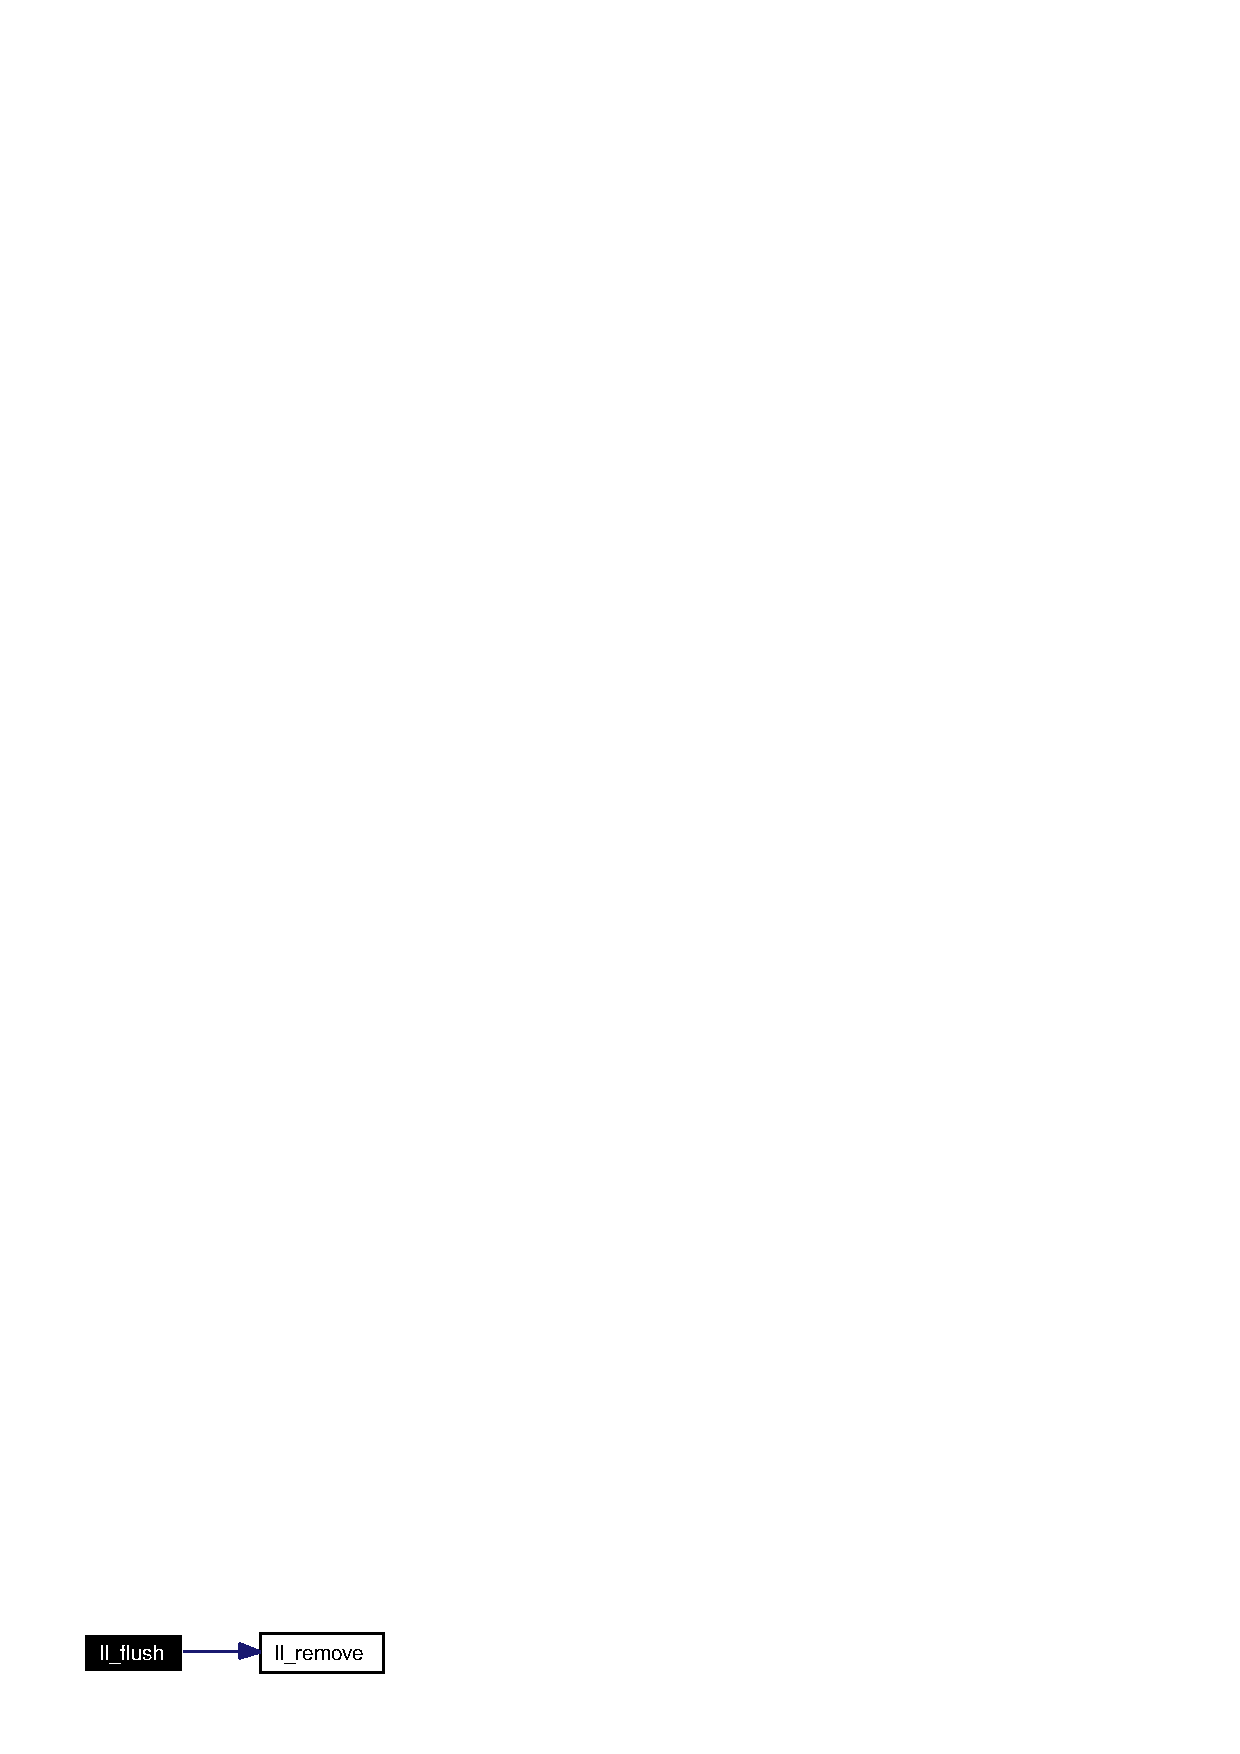
\includegraphics[width=94pt]{group__dbprim__link_ga11_cgraph}
\end{center}
\end{figure}
\hypertarget{group__dbprim__link_ga5}{
\index{dbprim_link@{dbprim\_\-link}!ll_init@{ll\_\-init}}
\index{ll_init@{ll\_\-init}!dbprim_link@{dbprim\_\-link}}
\subsubsection[ll\_\-init]{\setlength{\rightskip}{0pt plus 5cm}unsigned long ll\_\-init (\hyperlink{struct__link__head__s}{link\_\-head\_\-t} $\ast$ {\em list}, void $\ast$ {\em extra})}}
\label{group__dbprim__link_ga5}


This function dynamically initializes a linked list head.

\begin{Desc}
\item[Parameters:]
\begin{description}
\item[\mbox{$\leftarrow$} {\em list}]A pointer to a \hyperlink{group__dbprim__link_ga0}{link\_\-head\_\-t} to be initialized. \item[\mbox{$\leftarrow$} {\em extra}]A pointer to {\tt void} containing extra pointer data associated with the linked list.\end{description}
\end{Desc}
\begin{Desc}
\item[Return values:]
\begin{description}
\item[{\em DB\_\-ERR\_\-BADARGS}]A {\tt NULL} pointer was passed for {\tt list}.\end{description}
\end{Desc}


Definition at line 34 of file ll\_\-init.c.

References \_\-link\_\-head\_\-s::lh\_\-count, \_\-link\_\-head\_\-s::lh\_\-extra, \_\-link\_\-head\_\-s::lh\_\-first, \_\-link\_\-head\_\-s::lh\_\-last, \_\-link\_\-head\_\-s::lh\_\-magic, and LINK\_\-HEAD\_\-MAGIC.

Referenced by ht\_\-init(), ht\_\-resize(), and sh\_\-init().\hypertarget{group__dbprim__link_ga10}{
\index{dbprim_link@{dbprim\_\-link}!ll_iter@{ll\_\-iter}}
\index{ll_iter@{ll\_\-iter}!dbprim_link@{dbprim\_\-link}}
\subsubsection[ll\_\-iter]{\setlength{\rightskip}{0pt plus 5cm}unsigned long ll\_\-iter (\hyperlink{struct__link__head__s}{link\_\-head\_\-t} $\ast$ {\em list}, \hyperlink{struct__link__elem__s}{link\_\-elem\_\-t} $\ast$ {\em start}, \hyperlink{group__dbprim__link_ga2}{link\_\-iter\_\-t} {\em iter\_\-func}, void $\ast$ {\em extra}, unsigned long {\em flags})}}
\label{group__dbprim__link_ga10}


This function iterates over a linked list, executing the given {\tt iter\_\-func} for each entry.

\begin{Desc}
\item[Parameters:]
\begin{description}
\item[\mbox{$\leftarrow$} {\em list}]A pointer to a \hyperlink{group__dbprim__link_ga0}{link\_\-head\_\-t}. \item[\mbox{$\leftarrow$} {\em start}]A pointer to a \hyperlink{group__dbprim__link_ga1}{link\_\-elem\_\-t} describing where in the linked list to start. If {\tt NULL} is passed, the beginning of the list will be assumed. \item[\mbox{$\leftarrow$} {\em iter\_\-func}]A pointer to a callback function used to perform user-specified actions on an element in a linked list. {\tt NULL} is an invalid value. See the documentation for \hyperlink{group__dbprim__link_ga2}{link\_\-iter\_\-t} for more information. \item[\mbox{$\leftarrow$} {\em extra}]A {\tt void} pointer that will be passed to {\tt iter\_\-func}. \item[\mbox{$\leftarrow$} {\em flags}]If \hyperlink{group__dbprim_ga4}{DB\_\-FLAG\_\-REVERSE} is given, iteration will be done from the end of the list backwards towards the head.\end{description}
\end{Desc}
\begin{Desc}
\item[Return values:]
\begin{description}
\item[{\em DB\_\-ERR\_\-BADARGS}]An argument was invalid. \item[{\em DB\_\-ERR\_\-WRONGTABLE}]{\tt start} is not in this linked list.\end{description}
\end{Desc}


Definition at line 34 of file ll\_\-iter.c.

References DB\_\-FLAG\_\-REVERSE, \_\-link\_\-elem\_\-s::le\_\-head, \_\-link\_\-elem\_\-s::le\_\-next, \_\-link\_\-elem\_\-s::le\_\-prev, le\_\-verify, \_\-link\_\-head\_\-s::lh\_\-first, \_\-link\_\-head\_\-s::lh\_\-last, and ll\_\-verify.

Referenced by sh\_\-iter().\hypertarget{group__dbprim__link_ga7}{
\index{dbprim_link@{dbprim\_\-link}!ll_move@{ll\_\-move}}
\index{ll_move@{ll\_\-move}!dbprim_link@{dbprim\_\-link}}
\subsubsection[ll\_\-move]{\setlength{\rightskip}{0pt plus 5cm}unsigned long ll\_\-move (\hyperlink{struct__link__head__s}{link\_\-head\_\-t} $\ast$ {\em list}, \hyperlink{struct__link__elem__s}{link\_\-elem\_\-t} $\ast$ {\em elem}, \hyperlink{group__dbprim__link_ga4}{link\_\-loc\_\-t} {\em loc}, \hyperlink{struct__link__elem__s}{link\_\-elem\_\-t} $\ast$ {\em elem2})}}
\label{group__dbprim__link_ga7}


This function moves a specified element within the linked list.

\begin{Desc}
\item[Parameters:]
\begin{description}
\item[\mbox{$\leftarrow$} {\em list}]A pointer to a \hyperlink{group__dbprim__link_ga0}{link\_\-head\_\-t}. \item[\mbox{$\leftarrow$} {\em elem}]A pointer to the \hyperlink{group__dbprim__link_ga1}{link\_\-elem\_\-t} describing the element to be moved. \item[\mbox{$\leftarrow$} {\em loc}]A \hyperlink{group__dbprim__link_ga4}{link\_\-loc\_\-t} indicating where the entry should be moved to. \item[\mbox{$\leftarrow$} {\em elem2}]A pointer to a \hyperlink{group__dbprim__link_ga1}{link\_\-elem\_\-t} describing another element in the list if {\tt loc} is \hyperlink{group__dbprim__link_gga28a135}{LINK\_\-LOC\_\-BEFORE} or \hyperlink{group__dbprim__link_gga28a136}{LINK\_\-LOC\_\-AFTER}.\end{description}
\end{Desc}
\begin{Desc}
\item[Return values:]
\begin{description}
\item[{\em DB\_\-ERR\_\-BADARGS}]An argument was invalid. \item[{\em DB\_\-ERR\_\-BUSY}]{\tt new} and {\tt elem} are the same element. \item[{\em DB\_\-ERR\_\-WRONGTABLE}]{\tt new} or {\tt elem} are in a different list. \item[{\em DB\_\-ERR\_\-UNUSED}]{\tt new} or {\tt elem} are not in any list.\end{description}
\end{Desc}


Definition at line 35 of file ll\_\-move.c.

References \_\-link\_\-elem\_\-s::le\_\-head, \_\-link\_\-elem\_\-s::le\_\-next, \_\-link\_\-elem\_\-s::le\_\-prev, le\_\-verify, \_\-link\_\-head\_\-s::lh\_\-first, \_\-link\_\-head\_\-s::lh\_\-last, LINK\_\-LOC\_\-AFTER, LINK\_\-LOC\_\-BEFORE, LINK\_\-LOC\_\-HEAD, LINK\_\-LOC\_\-TAIL, and ll\_\-verify.

Referenced by sh\_\-move().\hypertarget{group__dbprim__link_ga8}{
\index{dbprim_link@{dbprim\_\-link}!ll_remove@{ll\_\-remove}}
\index{ll_remove@{ll\_\-remove}!dbprim_link@{dbprim\_\-link}}
\subsubsection[ll\_\-remove]{\setlength{\rightskip}{0pt plus 5cm}unsigned long ll\_\-remove (\hyperlink{struct__link__head__s}{link\_\-head\_\-t} $\ast$ {\em list}, \hyperlink{struct__link__elem__s}{link\_\-elem\_\-t} $\ast$ {\em elem})}}
\label{group__dbprim__link_ga8}


This function removes a specified element from a linked list.

\begin{Desc}
\item[Parameters:]
\begin{description}
\item[\mbox{$\leftarrow$} {\em list}]A pointer to a \hyperlink{group__dbprim__link_ga0}{link\_\-head\_\-t}. \item[\mbox{$\leftarrow$} {\em elem}]A pointer to the \hyperlink{group__dbprim__link_ga1}{link\_\-elem\_\-t} describing the element to be removed.\end{description}
\end{Desc}
\begin{Desc}
\item[Return values:]
\begin{description}
\item[{\em DB\_\-ERR\_\-BADARGS}]An argument was invalid. \item[{\em DB\_\-ERR\_\-UNUSED}]{\tt elem} is not in a linked list. \item[{\em DB\_\-ERR\_\-WRONGTABLE}]{\tt elem} is not in this linked list.\end{description}
\end{Desc}


Definition at line 34 of file ll\_\-remove.c.

References \_\-link\_\-elem\_\-s::le\_\-head, \_\-link\_\-elem\_\-s::le\_\-next, \_\-link\_\-elem\_\-s::le\_\-prev, le\_\-verify, \_\-link\_\-head\_\-s::lh\_\-count, \_\-link\_\-head\_\-s::lh\_\-first, \_\-link\_\-head\_\-s::lh\_\-last, and ll\_\-verify.

Referenced by \_\-smat\_\-alloc(), \_\-st\_\-remove(), ht\_\-move(), ht\_\-remove(), ht\_\-resize(), ll\_\-flush(), smat\_\-cleanup(), and st\_\-add().
\hypertarget{group__dbprim__hash}{
\section{Hash tables}
\label{group__dbprim__hash}\index{Hash tables@{Hash tables}}
}


\subsection{Detailed Description}
Hash tables are a basic data structure used in building databases. Hash tables provide a means of storing data such that an arbitrary entry may be looked up efficiently. This library implements a hash table that may optionally grow and shrink to provide maximum efficiency. The implementation is with two kinds of caller-allocated structures--a \hyperlink{group__dbprim__hash_a0}{hash\_\-table\_\-t} structure that describes the table and a \hyperlink{group__dbprim__hash_a1}{hash\_\-entry\_\-t} structure for each entry in the table. The library allocates a bucket array which must be released with the \hyperlink{group__dbprim__hash_a14}{ht\_\-free()} function when the hash table has been emptied. Additionally, the hash table may be manually resized with the \hyperlink{group__dbprim__hash_a13}{ht\_\-resize()} function.

Entries may be added to and removed from the table using the \hyperlink{group__dbprim__hash_a7}{ht\_\-add()} and \hyperlink{group__dbprim__hash_a9}{ht\_\-remove()} functions. Additionally, the key on a given entry may be changed using the \hyperlink{group__dbprim__hash_a8}{ht\_\-move()} function. Of course, any given entry may be looked up using the \hyperlink{group__dbprim__hash_a10}{ht\_\-find()} function, and \hyperlink{group__dbprim__hash_a11}{ht\_\-iter()} will execute a user-defined function for each entry in the hash table (in an unspecified order). The \hyperlink{group__dbprim__hash_a12}{ht\_\-flush()} function will remove all entries from the hash table, optionally executing a user-specified clean-up function. 

\subsection*{Defines}
\begin{CompactItemize}
\item 
\#define \hyperlink{group__dbprim__hash_a16}{HASH\_\-FLAG\_\-AUTOGROW}
\begin{CompactList}\small\item\em Flag permitting a hash table to automatically grow. \item\end{CompactList}\item 
\#define \hyperlink{group__dbprim__hash_a17}{HASH\_\-FLAG\_\-AUTOSHRINK}
\begin{CompactList}\small\item\em Flag permitting a hash table to automatically shrink. \item\end{CompactList}\item 
\#define \hyperlink{group__dbprim__hash_a18}{HASH\_\-TABLE\_\-INIT}(flags, func, comp, resize, extra)
\begin{CompactList}\small\item\em Hash table static initializer. \item\end{CompactList}\item 
\#define \hyperlink{group__dbprim__hash_a19}{ht\_\-verify}(table)
\begin{CompactList}\small\item\em Hash table verification macro. \item\end{CompactList}\item 
\#define \hyperlink{group__dbprim__hash_a20}{ht\_\-flags}(table)
\begin{CompactList}\small\item\em Hash table flags. \item\end{CompactList}\item 
\#define \hyperlink{group__dbprim__hash_a21}{ht\_\-frozen}(table)
\begin{CompactList}\small\item\em Determine if a hash table is frozen. \item\end{CompactList}\item 
\#define \hyperlink{group__dbprim__hash_a22}{ht\_\-modulus}(table)
\begin{CompactList}\small\item\em Hash table modulus. \item\end{CompactList}\item 
\#define \hyperlink{group__dbprim__hash_a23}{ht\_\-count}(table)
\begin{CompactList}\small\item\em Hash table count. \item\end{CompactList}\item 
\#define \hyperlink{group__dbprim__hash_a24}{ht\_\-func}(table)
\begin{CompactList}\small\item\em Hash table hash function. \item\end{CompactList}\item 
\#define \hyperlink{group__dbprim__hash_a25}{ht\_\-comp}(table)
\begin{CompactList}\small\item\em Hash table comparison function. \item\end{CompactList}\item 
\#define \hyperlink{group__dbprim__hash_a26}{ht\_\-rsize}(table)
\begin{CompactList}\small\item\em Hash table resize callback function. \item\end{CompactList}\item 
\#define \hyperlink{group__dbprim__hash_a27}{ht\_\-extra}(table)
\begin{CompactList}\small\item\em Extra pointer data in a hash table. \item\end{CompactList}\item 
\#define \hyperlink{group__dbprim__hash_a28}{ht\_\-size}(table)
\begin{CompactList}\small\item\em Hash table memory size. \item\end{CompactList}\item 
\#define \hyperlink{group__dbprim__hash_a29}{HASH\_\-ENTRY\_\-INIT}(value)
\begin{CompactList}\small\item\em Hash table entry static initializer. \item\end{CompactList}\item 
\#define \hyperlink{group__dbprim__hash_a30}{he\_\-verify}(entry)
\begin{CompactList}\small\item\em Hash table entry verification macro. \item\end{CompactList}\item 
\#define \hyperlink{group__dbprim__hash_a31}{he\_\-link}(entry)
\begin{CompactList}\small\item\em Hash table entry linked list element. \item\end{CompactList}\item 
\#define \hyperlink{group__dbprim__hash_a32}{he\_\-flags}(entry)
\begin{CompactList}\small\item\em Hash table entry flags. \item\end{CompactList}\item 
\#define \hyperlink{group__dbprim__hash_a33}{he\_\-table}(entry)
\begin{CompactList}\small\item\em Hash table entry table pointer. \item\end{CompactList}\item 
\#define \hyperlink{group__dbprim__hash_a34}{he\_\-hash}(entry)
\begin{CompactList}\small\item\em Hash table entry hash value. \item\end{CompactList}\item 
\#define \hyperlink{group__dbprim__hash_a35}{he\_\-key}(entry)
\begin{CompactList}\small\item\em Hash table entry key pointer. \item\end{CompactList}\item 
\#define \hyperlink{group__dbprim__hash_a36}{he\_\-value}(entry)
\begin{CompactList}\small\item\em Hash table entry value pointer. \item\end{CompactList}\item 
\#define \hyperlink{group__dbprim__hash_a37}{st\_\-rsize}(table)
\begin{CompactList}\small\item\em Sparse matrix table resize callback function. \item\end{CompactList}\end{CompactItemize}
\subsection*{Typedefs}
\begin{CompactItemize}
\item 
typedef \_\-hash\_\-table\_\-s \hyperlink{group__dbprim__hash_a0}{hash\_\-table\_\-t}
\begin{CompactList}\small\item\em Hash table. \item\end{CompactList}\item 
typedef \_\-hash\_\-entry\_\-s \hyperlink{group__dbprim__hash_a1}{hash\_\-entry\_\-t}
\begin{CompactList}\small\item\em Hash table entry. \item\end{CompactList}\item 
typedef unsigned long($\ast$ \hyperlink{group__dbprim__hash_a2}{hash\_\-iter\_\-t} )(\hyperlink{dbprim_8h_a0}{hash\_\-table\_\-t} $\ast$, \hyperlink{dbprim_8h_a1}{hash\_\-entry\_\-t} $\ast$, void $\ast$)
\begin{CompactList}\small\item\em Hash table iteration callback. \item\end{CompactList}\item 
typedef unsigned long($\ast$ \hyperlink{group__dbprim__hash_a3}{hash\_\-func\_\-t} )(\hyperlink{dbprim_8h_a0}{hash\_\-table\_\-t} $\ast$, \hyperlink{dbprim_8h_a0}{db\_\-key\_\-t} $\ast$)
\begin{CompactList}\small\item\em Hash function callback. \item\end{CompactList}\item 
typedef unsigned long($\ast$ \hyperlink{group__dbprim__hash_a4}{hash\_\-comp\_\-t} )(\hyperlink{dbprim_8h_a0}{hash\_\-table\_\-t} $\ast$, \hyperlink{dbprim_8h_a0}{db\_\-key\_\-t} $\ast$, \hyperlink{dbprim_8h_a0}{db\_\-key\_\-t} $\ast$)
\begin{CompactList}\small\item\em Hash table comparison callback. \item\end{CompactList}\item 
typedef unsigned long($\ast$ \hyperlink{group__dbprim__hash_a5}{hash\_\-resize\_\-t} )(\hyperlink{dbprim_8h_a0}{hash\_\-table\_\-t} $\ast$, unsigned long)
\begin{CompactList}\small\item\em Hash table resize callback. \item\end{CompactList}\end{CompactItemize}
\subsection*{Functions}
\begin{CompactItemize}
\item 
unsigned long \hyperlink{group__dbprim__hash_a6}{ht\_\-init} (\hyperlink{dbprim_8h_a0}{hash\_\-table\_\-t} $\ast$table, unsigned long flags, \hyperlink{dbprim_8h_a3}{hash\_\-func\_\-t} func, \hyperlink{dbprim_8h_a4}{hash\_\-comp\_\-t} comp, \hyperlink{dbprim_8h_a5}{hash\_\-resize\_\-t} resize, void $\ast$extra, unsigned long init\_\-mod)
\begin{CompactList}\small\item\em Dynamically initialize a hash table. \item\end{CompactList}\item 
unsigned long \hyperlink{group__dbprim__hash_a7}{ht\_\-add} (\hyperlink{dbprim_8h_a0}{hash\_\-table\_\-t} $\ast$table, \hyperlink{dbprim_8h_a1}{hash\_\-entry\_\-t} $\ast$entry, \hyperlink{dbprim_8h_a0}{db\_\-key\_\-t} $\ast$key)
\begin{CompactList}\small\item\em Add an entry to a hash table. \item\end{CompactList}\item 
unsigned long \hyperlink{group__dbprim__hash_a8}{ht\_\-move} (\hyperlink{dbprim_8h_a0}{hash\_\-table\_\-t} $\ast$table, \hyperlink{dbprim_8h_a1}{hash\_\-entry\_\-t} $\ast$entry, \hyperlink{dbprim_8h_a0}{db\_\-key\_\-t} $\ast$key)
\begin{CompactList}\small\item\em Move an entry in the hash table. \item\end{CompactList}\item 
unsigned long \hyperlink{group__dbprim__hash_a9}{ht\_\-remove} (\hyperlink{dbprim_8h_a0}{hash\_\-table\_\-t} $\ast$table, \hyperlink{dbprim_8h_a1}{hash\_\-entry\_\-t} $\ast$entry)
\begin{CompactList}\small\item\em Remove an element from a hash table. \item\end{CompactList}\item 
unsigned long \hyperlink{group__dbprim__hash_a10}{ht\_\-find} (\hyperlink{dbprim_8h_a0}{hash\_\-table\_\-t} $\ast$table, \hyperlink{dbprim_8h_a1}{hash\_\-entry\_\-t} $\ast$$\ast$entry\_\-p, \hyperlink{dbprim_8h_a0}{db\_\-key\_\-t} $\ast$key)
\begin{CompactList}\small\item\em Find an entry in a hash table. \item\end{CompactList}\item 
unsigned long \hyperlink{group__dbprim__hash_a11}{ht\_\-iter} (\hyperlink{dbprim_8h_a0}{hash\_\-table\_\-t} $\ast$table, \hyperlink{dbprim_8h_a2}{hash\_\-iter\_\-t} iter\_\-func, void $\ast$extra)
\begin{CompactList}\small\item\em Iterate over each entry in a hash table. \item\end{CompactList}\item 
unsigned long \hyperlink{group__dbprim__hash_a12}{ht\_\-flush} (\hyperlink{dbprim_8h_a0}{hash\_\-table\_\-t} $\ast$table, \hyperlink{dbprim_8h_a2}{hash\_\-iter\_\-t} flush\_\-func, void $\ast$extra)
\begin{CompactList}\small\item\em Flush a hash table. \item\end{CompactList}\item 
unsigned long \hyperlink{group__dbprim__hash_a13}{ht\_\-resize} (\hyperlink{dbprim_8h_a0}{hash\_\-table\_\-t} $\ast$table, unsigned long new\_\-size)
\begin{CompactList}\small\item\em Resize a hash table. \item\end{CompactList}\item 
unsigned long \hyperlink{group__dbprim__hash_a14}{ht\_\-free} (\hyperlink{dbprim_8h_a0}{hash\_\-table\_\-t} $\ast$table)
\begin{CompactList}\small\item\em Free memory used by an empty hash table. \item\end{CompactList}\item 
unsigned long \hyperlink{group__dbprim__hash_a15}{he\_\-init} (\hyperlink{dbprim_8h_a1}{hash\_\-entry\_\-t} $\ast$entry, void $\ast$value)
\begin{CompactList}\small\item\em Dynamically initialize a hash table entry. \item\end{CompactList}\end{CompactItemize}


\subsection{Define Documentation}
\hypertarget{group__dbprim__hash_a29}{
\index{dbprim_hash@{dbprim\_\-hash}!HASH_ENTRY_INIT@{HASH\_\-ENTRY\_\-INIT}}
\index{HASH_ENTRY_INIT@{HASH\_\-ENTRY\_\-INIT}!dbprim_hash@{dbprim\_\-hash}}
\subsubsection[HASH\_\-ENTRY\_\-INIT]{\setlength{\rightskip}{0pt plus 5cm}\#define HASH\_\-ENTRY\_\-INIT(value)}}
\label{group__dbprim__hash_a29}


This macro statically initializes a \hyperlink{group__dbprim__hash_a1}{hash\_\-entry\_\-t}.

\begin{Desc}
\item[Parameters:]
\begin{description}
\item[{\em value}]A pointer to {\tt void} representing the object associated with the entry. \end{description}
\end{Desc}
\hypertarget{group__dbprim__hash_a16}{
\index{dbprim_hash@{dbprim\_\-hash}!HASH_FLAG_AUTOGROW@{HASH\_\-FLAG\_\-AUTOGROW}}
\index{HASH_FLAG_AUTOGROW@{HASH\_\-FLAG\_\-AUTOGROW}!dbprim_hash@{dbprim\_\-hash}}
\subsubsection[HASH\_\-FLAG\_\-AUTOGROW]{\setlength{\rightskip}{0pt plus 5cm}\#define HASH\_\-FLAG\_\-AUTOGROW}}
\label{group__dbprim__hash_a16}


If passed in to \hyperlink{group__dbprim__hash_a18}{HASH\_\-TABLE\_\-INIT()} or \hyperlink{group__dbprim__hash_a6}{ht\_\-init()}, allows the hash table to grow automatically. \hypertarget{group__dbprim__hash_a17}{
\index{dbprim_hash@{dbprim\_\-hash}!HASH_FLAG_AUTOSHRINK@{HASH\_\-FLAG\_\-AUTOSHRINK}}
\index{HASH_FLAG_AUTOSHRINK@{HASH\_\-FLAG\_\-AUTOSHRINK}!dbprim_hash@{dbprim\_\-hash}}
\subsubsection[HASH\_\-FLAG\_\-AUTOSHRINK]{\setlength{\rightskip}{0pt plus 5cm}\#define HASH\_\-FLAG\_\-AUTOSHRINK}}
\label{group__dbprim__hash_a17}


If passed in to \hyperlink{group__dbprim__hash_a18}{HASH\_\-TABLE\_\-INIT()} or \hyperlink{group__dbprim__hash_a6}{ht\_\-init()}, allows the hash table to shrink automatically. \hypertarget{group__dbprim__hash_a18}{
\index{dbprim_hash@{dbprim\_\-hash}!HASH_TABLE_INIT@{HASH\_\-TABLE\_\-INIT}}
\index{HASH_TABLE_INIT@{HASH\_\-TABLE\_\-INIT}!dbprim_hash@{dbprim\_\-hash}}
\subsubsection[HASH\_\-TABLE\_\-INIT]{\setlength{\rightskip}{0pt plus 5cm}\#define HASH\_\-TABLE\_\-INIT(flags, func, comp, resize, extra)}}
\label{group__dbprim__hash_a18}


This macro statically initializes a \hyperlink{group__dbprim__hash_a0}{hash\_\-table\_\-t}.

\begin{Desc}
\item[Parameters:]
\begin{description}
\item[{\em flags}]A bit-wise OR of \hyperlink{group__dbprim__hash_a16}{HASH\_\-FLAG\_\-AUTOGROW} and \hyperlink{group__dbprim__hash_a17}{HASH\_\-FLAG\_\-AUTOSHRINK}. If neither behavior is desired, use 0. \item[{\em func}]A \hyperlink{group__dbprim__hash_a3}{hash\_\-func\_\-t} function pointer for a hash function. \item[{\em comp}]A \hyperlink{group__dbprim__hash_a4}{hash\_\-comp\_\-t} function pointer for a comparison function. \item[{\em resize}]A \hyperlink{group__dbprim__hash_a5}{hash\_\-resize\_\-t} function pointer for determining whether resizing is permitted and/or for notification of the resize. \item[{\em extra}]Extra pointer data that should be associated with the hash table. \end{description}
\end{Desc}
\hypertarget{group__dbprim__hash_a32}{
\index{dbprim_hash@{dbprim\_\-hash}!he_flags@{he\_\-flags}}
\index{he_flags@{he\_\-flags}!dbprim_hash@{dbprim\_\-hash}}
\subsubsection[he\_\-flags]{\setlength{\rightskip}{0pt plus 5cm}\#define he\_\-flags(entry)}}
\label{group__dbprim__hash_a32}


This macro retrieves a set of user-defined flags associated with the entry. It may be used as an lvalue to set those flags.

\begin{Desc}
\item[Parameters:]
\begin{description}
\item[{\em entry}]A pointer to a \hyperlink{group__dbprim__hash_a1}{hash\_\-entry\_\-t}.\end{description}
\end{Desc}
\begin{Desc}
\item[Returns:]An {\tt unsigned long} containing the flags associated with the entry. \end{Desc}
\hypertarget{group__dbprim__hash_a34}{
\index{dbprim_hash@{dbprim\_\-hash}!he_hash@{he\_\-hash}}
\index{he_hash@{he\_\-hash}!dbprim_hash@{dbprim\_\-hash}}
\subsubsection[he\_\-hash]{\setlength{\rightskip}{0pt plus 5cm}\#define he\_\-hash(entry)}}
\label{group__dbprim__hash_a34}


This macro retrieves the hash value of the given hash entry. If the hash table has been resized, this value may not be the same as a previous value.

\begin{Desc}
\item[Parameters:]
\begin{description}
\item[{\em entry}]A pointer to a \hyperlink{group__dbprim__hash_a1}{hash\_\-entry\_\-t}.\end{description}
\end{Desc}
\begin{Desc}
\item[Returns:]An {\tt unsigned long} containing the hash code for the entry. \end{Desc}
\hypertarget{group__dbprim__hash_a35}{
\index{dbprim_hash@{dbprim\_\-hash}!he_key@{he\_\-key}}
\index{he_key@{he\_\-key}!dbprim_hash@{dbprim\_\-hash}}
\subsubsection[he\_\-key]{\setlength{\rightskip}{0pt plus 5cm}\#define he\_\-key(entry)}}
\label{group__dbprim__hash_a35}


This macro retrieves the key associated with the hash table entry.

\begin{Desc}
\item[Parameters:]
\begin{description}
\item[{\em entry}]A pointer to a \hyperlink{group__dbprim__hash_a1}{hash\_\-entry\_\-t}.\end{description}
\end{Desc}
\begin{Desc}
\item[Returns:]A pointer to a \hyperlink{group__dbprim_a0}{db\_\-key\_\-t}. \end{Desc}
\hypertarget{group__dbprim__hash_a31}{
\index{dbprim_hash@{dbprim\_\-hash}!he_link@{he\_\-link}}
\index{he_link@{he\_\-link}!dbprim_hash@{dbprim\_\-hash}}
\subsubsection[he\_\-link]{\setlength{\rightskip}{0pt plus 5cm}\#define he\_\-link(entry)}}
\label{group__dbprim__hash_a31}


This macro provides access to the linked list element buried in the hash table entry. It should $\ast$not$\ast$ be used on entries currently in a hash table. The purpose of this macro is to allow an object containing a hash table entry to be placed upon a free list.

\begin{Desc}
\item[Parameters:]
\begin{description}
\item[{\em entry}]A pointer to a \hyperlink{group__dbprim__hash_a1}{hash\_\-entry\_\-t}.\end{description}
\end{Desc}
\begin{Desc}
\item[Returns:]A pointer to a \hyperlink{group__dbprim__link_a1}{link\_\-elem\_\-t}. \end{Desc}
\hypertarget{group__dbprim__hash_a33}{
\index{dbprim_hash@{dbprim\_\-hash}!he_table@{he\_\-table}}
\index{he_table@{he\_\-table}!dbprim_hash@{dbprim\_\-hash}}
\subsubsection[he\_\-table]{\setlength{\rightskip}{0pt plus 5cm}\#define he\_\-table(entry)}}
\label{group__dbprim__hash_a33}


This macro retrieves a pointer to the hash table the entry is in.

\begin{Desc}
\item[Parameters:]
\begin{description}
\item[{\em entry}]A pointer to a \hyperlink{group__dbprim__hash_a1}{hash\_\-entry\_\-t}.\end{description}
\end{Desc}
\begin{Desc}
\item[Returns:]A pointer to a \hyperlink{group__dbprim__hash_a0}{hash\_\-table\_\-t}. \end{Desc}
\hypertarget{group__dbprim__hash_a36}{
\index{dbprim_hash@{dbprim\_\-hash}!he_value@{he\_\-value}}
\index{he_value@{he\_\-value}!dbprim_hash@{dbprim\_\-hash}}
\subsubsection[he\_\-value]{\setlength{\rightskip}{0pt plus 5cm}\#define he\_\-value(entry)}}
\label{group__dbprim__hash_a36}


This macro retrieves the value associated with the hash table entry. It may be treated as an lvalue to change that value. Care should be taken when using this option.

\begin{Desc}
\item[Parameters:]
\begin{description}
\item[{\em entry}]A pointer to a \hyperlink{group__dbprim__hash_a1}{hash\_\-entry\_\-t}.\end{description}
\end{Desc}
\begin{Desc}
\item[Returns:]A pointer to {\tt void} representing the value associated with this entry. \end{Desc}
\hypertarget{group__dbprim__hash_a30}{
\index{dbprim_hash@{dbprim\_\-hash}!he_verify@{he\_\-verify}}
\index{he_verify@{he\_\-verify}!dbprim_hash@{dbprim\_\-hash}}
\subsubsection[he\_\-verify]{\setlength{\rightskip}{0pt plus 5cm}\#define he\_\-verify(entry)}}
\label{group__dbprim__hash_a30}


This macro verifies that a given pointer actually does point to a hash table entry.

\begin{Desc}
\item[Warning:]This macro may evaluate the {\tt entry} argument twice.\end{Desc}
\begin{Desc}
\item[Parameters:]
\begin{description}
\item[{\em entry}]A pointer to a \hyperlink{group__dbprim__hash_a1}{hash\_\-entry\_\-t}.\end{description}
\end{Desc}
\begin{Desc}
\item[Returns:]Boolean true if {\tt entry} is a valid hash table entry or false otherwise. \end{Desc}
\hypertarget{group__dbprim__hash_a25}{
\index{dbprim_hash@{dbprim\_\-hash}!ht_comp@{ht\_\-comp}}
\index{ht_comp@{ht\_\-comp}!dbprim_hash@{dbprim\_\-hash}}
\subsubsection[ht\_\-comp]{\setlength{\rightskip}{0pt plus 5cm}\#define ht\_\-comp(table)}}
\label{group__dbprim__hash_a25}


This macro retrieves the comparison function pointer.

\begin{Desc}
\item[Parameters:]
\begin{description}
\item[{\em table}]A pointer to a \hyperlink{group__dbprim__hash_a0}{hash\_\-table\_\-t}.\end{description}
\end{Desc}
\begin{Desc}
\item[Returns:]A \hyperlink{group__dbprim__hash_a4}{hash\_\-comp\_\-t}. \end{Desc}
\hypertarget{group__dbprim__hash_a23}{
\index{dbprim_hash@{dbprim\_\-hash}!ht_count@{ht\_\-count}}
\index{ht_count@{ht\_\-count}!dbprim_hash@{dbprim\_\-hash}}
\subsubsection[ht\_\-count]{\setlength{\rightskip}{0pt plus 5cm}\#define ht\_\-count(table)}}
\label{group__dbprim__hash_a23}


This macro retrieves the total number of items actually in the hash table.

\begin{Desc}
\item[Parameters:]
\begin{description}
\item[{\em table}]A pointer to a \hyperlink{group__dbprim__hash_a0}{hash\_\-table\_\-t}.\end{description}
\end{Desc}
\begin{Desc}
\item[Returns:]An {\tt unsigned long} containing a count of the number of items in the hash table. \end{Desc}
\hypertarget{group__dbprim__hash_a27}{
\index{dbprim_hash@{dbprim\_\-hash}!ht_extra@{ht\_\-extra}}
\index{ht_extra@{ht\_\-extra}!dbprim_hash@{dbprim\_\-hash}}
\subsubsection[ht\_\-extra]{\setlength{\rightskip}{0pt plus 5cm}\#define ht\_\-extra(table)}}
\label{group__dbprim__hash_a27}


This macro retrieves the extra pointer data associated with a particular hash table.

\begin{Desc}
\item[Parameters:]
\begin{description}
\item[{\em table}]A pointer to a \hyperlink{group__dbprim__hash_a0}{hash\_\-table\_\-t}.\end{description}
\end{Desc}
\begin{Desc}
\item[Returns:]A pointer to {\tt void}. \end{Desc}
\hypertarget{group__dbprim__hash_a20}{
\index{dbprim_hash@{dbprim\_\-hash}!ht_flags@{ht\_\-flags}}
\index{ht_flags@{ht\_\-flags}!dbprim_hash@{dbprim\_\-hash}}
\subsubsection[ht\_\-flags]{\setlength{\rightskip}{0pt plus 5cm}\#define ht\_\-flags(table)}}
\label{group__dbprim__hash_a20}


This macro retrieves the flags associated with the hash table. Only \hyperlink{group__dbprim__hash_a16}{HASH\_\-FLAG\_\-AUTOGROW} and \hyperlink{group__dbprim__hash_a17}{HASH\_\-FLAG\_\-AUTOSHRINK} have any meaning to the application; all other bits are reserved for use in the library. This macro may be used as an lvalue, but care must be taken to avoid modifying the library-specific bits.

\begin{Desc}
\item[Parameters:]
\begin{description}
\item[{\em table}]A pointer to a \hyperlink{group__dbprim__hash_a0}{hash\_\-table\_\-t}.\end{description}
\end{Desc}
\begin{Desc}
\item[Returns:]An {\tt unsigned long} containing the flags for the hash table. \end{Desc}
\hypertarget{group__dbprim__hash_a21}{
\index{dbprim_hash@{dbprim\_\-hash}!ht_frozen@{ht\_\-frozen}}
\index{ht_frozen@{ht\_\-frozen}!dbprim_hash@{dbprim\_\-hash}}
\subsubsection[ht\_\-frozen]{\setlength{\rightskip}{0pt plus 5cm}\#define ht\_\-frozen(table)}}
\label{group__dbprim__hash_a21}


This macro returns a non-zero value if the table is currently frozen. The hash table may be frozen if there is an iteration in progress.

\begin{Desc}
\item[Parameters:]
\begin{description}
\item[{\em table}]A pointer to a \hyperlink{group__dbprim__hash_a0}{hash\_\-table\_\-t}.\end{description}
\end{Desc}
\begin{Desc}
\item[Returns:]A zero value if the table is not frozen or a non-zero value if the table is frozen. \end{Desc}
\hypertarget{group__dbprim__hash_a24}{
\index{dbprim_hash@{dbprim\_\-hash}!ht_func@{ht\_\-func}}
\index{ht_func@{ht\_\-func}!dbprim_hash@{dbprim\_\-hash}}
\subsubsection[ht\_\-func]{\setlength{\rightskip}{0pt plus 5cm}\#define ht\_\-func(table)}}
\label{group__dbprim__hash_a24}


This macro retrieves the hash function pointer.

\begin{Desc}
\item[Parameters:]
\begin{description}
\item[{\em table}]A pointer to a \hyperlink{group__dbprim__hash_a0}{hash\_\-table\_\-t}.\end{description}
\end{Desc}
\begin{Desc}
\item[Returns:]A \hyperlink{group__dbprim__hash_a3}{hash\_\-func\_\-t}. \end{Desc}
\hypertarget{group__dbprim__hash_a22}{
\index{dbprim_hash@{dbprim\_\-hash}!ht_modulus@{ht\_\-modulus}}
\index{ht_modulus@{ht\_\-modulus}!dbprim_hash@{dbprim\_\-hash}}
\subsubsection[ht\_\-modulus]{\setlength{\rightskip}{0pt plus 5cm}\#define ht\_\-modulus(table)}}
\label{group__dbprim__hash_a22}


This macro retrieves the number of buckets allocated for the hash table. An application may wish to save this value between invocations to avoid the overhead of growing the table while filling it with data.

\begin{Desc}
\item[Parameters:]
\begin{description}
\item[{\em table}]A pointer to a \hyperlink{group__dbprim__hash_a0}{hash\_\-table\_\-t}.\end{description}
\end{Desc}
\begin{Desc}
\item[Returns:]An {\tt unsigned long} containing the number of buckets allocated for the hash table. \end{Desc}
\hypertarget{group__dbprim__hash_a26}{
\index{dbprim_hash@{dbprim\_\-hash}!ht_rsize@{ht\_\-rsize}}
\index{ht_rsize@{ht\_\-rsize}!dbprim_hash@{dbprim\_\-hash}}
\subsubsection[ht\_\-rsize]{\setlength{\rightskip}{0pt plus 5cm}\#define ht\_\-rsize(table)}}
\label{group__dbprim__hash_a26}


This macro retrieves the resize callback function pointer.

\begin{Desc}
\item[Parameters:]
\begin{description}
\item[{\em table}]A pointer to a \hyperlink{group__dbprim__hash_a0}{hash\_\-table\_\-t}.\end{description}
\end{Desc}
\begin{Desc}
\item[Returns:]A \hyperlink{group__dbprim__hash_a5}{hash\_\-resize\_\-t}. \end{Desc}
\hypertarget{group__dbprim__hash_a28}{
\index{dbprim_hash@{dbprim\_\-hash}!ht_size@{ht\_\-size}}
\index{ht_size@{ht\_\-size}!dbprim_hash@{dbprim\_\-hash}}
\subsubsection[ht\_\-size]{\setlength{\rightskip}{0pt plus 5cm}\#define ht\_\-size(table)}}
\label{group__dbprim__hash_a28}


This macro returns the physical size of the bucket array allocated by the library for this hash table.

\begin{Desc}
\item[Parameters:]
\begin{description}
\item[{\em table}]A pointer to a \hyperlink{group__dbprim__hash_a0}{hash\_\-table\_\-t}.\end{description}
\end{Desc}
\begin{Desc}
\item[Returns:]A {\tt size\_\-t}. \end{Desc}
\hypertarget{group__dbprim__hash_a19}{
\index{dbprim_hash@{dbprim\_\-hash}!ht_verify@{ht\_\-verify}}
\index{ht_verify@{ht\_\-verify}!dbprim_hash@{dbprim\_\-hash}}
\subsubsection[ht\_\-verify]{\setlength{\rightskip}{0pt plus 5cm}\#define ht\_\-verify(table)}}
\label{group__dbprim__hash_a19}


This macro verifies that a given pointer actually does point to a hash table.

\begin{Desc}
\item[Warning:]This macro may evaluate the {\tt table} argument twice.\end{Desc}
\begin{Desc}
\item[Parameters:]
\begin{description}
\item[{\em table}]A pointer to a \hyperlink{group__dbprim__hash_a0}{hash\_\-table\_\-t}.\end{description}
\end{Desc}
\begin{Desc}
\item[Returns:]Boolean true if {\tt table} is a valid hash table or false otherwise. \end{Desc}
\hypertarget{group__dbprim__hash_a37}{
\index{dbprim_hash@{dbprim\_\-hash}!st_rsize@{st\_\-rsize}}
\index{st_rsize@{st\_\-rsize}!dbprim_hash@{dbprim\_\-hash}}
\subsubsection[st\_\-rsize]{\setlength{\rightskip}{0pt plus 5cm}\#define st\_\-rsize(table)}}
\label{group__dbprim__hash_a37}


This macro retrieves the resize callback function pointer.

\begin{Desc}
\item[Parameters:]
\begin{description}
\item[{\em table}]A pointer to a \hyperlink{group__dbprim__smat_a0}{smat\_\-table\_\-t}.\end{description}
\end{Desc}
\begin{Desc}
\item[Returns:]A \hyperlink{group__dbprim__smat_a3}{smat\_\-resize\_\-t}. \end{Desc}


\subsection{Typedef Documentation}
\hypertarget{group__dbprim__hash_a4}{
\index{dbprim_hash@{dbprim\_\-hash}!hash_comp_t@{hash\_\-comp\_\-t}}
\index{hash_comp_t@{hash\_\-comp\_\-t}!dbprim_hash@{dbprim\_\-hash}}
\subsubsection[hash\_\-comp\_\-t]{\setlength{\rightskip}{0pt plus 5cm}typedef unsigned long($\ast$ \hyperlink{dbprim_8h_a4}{hash\_\-comp\_\-t})(\hyperlink{dbprim_8h_a0}{hash\_\-table\_\-t} $\ast$, \hyperlink{dbprim_8h_a0}{db\_\-key\_\-t} $\ast$, \hyperlink{dbprim_8h_a0}{db\_\-key\_\-t} $\ast$)}}
\label{group__dbprim__hash_a4}


This function pointer references a callback used to compare entries in a hash table. It should return 0 for identical entries and non-zero otherwise. No assumptions should be made about the order in which the two keys are passed to this function. \hypertarget{group__dbprim__hash_a1}{
\index{dbprim_hash@{dbprim\_\-hash}!hash_entry_t@{hash\_\-entry\_\-t}}
\index{hash_entry_t@{hash\_\-entry\_\-t}!dbprim_hash@{dbprim\_\-hash}}
\subsubsection[hash\_\-entry\_\-t]{\setlength{\rightskip}{0pt plus 5cm}typedef struct \_\-hash\_\-entry\_\-s \hyperlink{dbprim_8h_a1}{hash\_\-entry\_\-t}}}
\label{group__dbprim__hash_a1}


This structure represents a single entry of a hash table. \hypertarget{group__dbprim__hash_a3}{
\index{dbprim_hash@{dbprim\_\-hash}!hash_func_t@{hash\_\-func\_\-t}}
\index{hash_func_t@{hash\_\-func\_\-t}!dbprim_hash@{dbprim\_\-hash}}
\subsubsection[hash\_\-func\_\-t]{\setlength{\rightskip}{0pt plus 5cm}typedef unsigned long($\ast$ \hyperlink{dbprim_8h_a3}{hash\_\-func\_\-t})(\hyperlink{dbprim_8h_a0}{hash\_\-table\_\-t} $\ast$, \hyperlink{dbprim_8h_a0}{db\_\-key\_\-t} $\ast$)}}
\label{group__dbprim__hash_a3}


This function is associated with a hash table, and is responsible for generating a hash value. The full 32-bit range of an {\tt unsigned long} should be used--do $\ast$not$\ast$ reduce the hash value by the modulus of the hash table. \hypertarget{group__dbprim__hash_a2}{
\index{dbprim_hash@{dbprim\_\-hash}!hash_iter_t@{hash\_\-iter\_\-t}}
\index{hash_iter_t@{hash\_\-iter\_\-t}!dbprim_hash@{dbprim\_\-hash}}
\subsubsection[hash\_\-iter\_\-t]{\setlength{\rightskip}{0pt plus 5cm}typedef unsigned long($\ast$ \hyperlink{dbprim_8h_a2}{hash\_\-iter\_\-t})(\hyperlink{dbprim_8h_a0}{hash\_\-table\_\-t} $\ast$, \hyperlink{dbprim_8h_a1}{hash\_\-entry\_\-t} $\ast$, void $\ast$)}}
\label{group__dbprim__hash_a2}


This function pointer references a callback used by \hyperlink{group__dbprim__hash_a11}{ht\_\-iter()} and \hyperlink{group__dbprim__hash_a12}{ht\_\-flush()}. It should return 0 for success. A non-zero return value will terminate the operation and will become the return value of the \hyperlink{group__dbprim__hash_a11}{ht\_\-iter()} or \hyperlink{group__dbprim__hash_a12}{ht\_\-flush()} call. \hypertarget{group__dbprim__hash_a5}{
\index{dbprim_hash@{dbprim\_\-hash}!hash_resize_t@{hash\_\-resize\_\-t}}
\index{hash_resize_t@{hash\_\-resize\_\-t}!dbprim_hash@{dbprim\_\-hash}}
\subsubsection[hash\_\-resize\_\-t]{\setlength{\rightskip}{0pt plus 5cm}typedef unsigned long($\ast$ \hyperlink{dbprim_8h_a5}{hash\_\-resize\_\-t})(\hyperlink{dbprim_8h_a0}{hash\_\-table\_\-t} $\ast$, unsigned long)}}
\label{group__dbprim__hash_a5}


This function pointer references a callback that will be called with both the old and new hash table sizes whenever a hash table is resized. It should return non-zero only when the resize should be inhibited. \hypertarget{group__dbprim__hash_a0}{
\index{dbprim_hash@{dbprim\_\-hash}!hash_table_t@{hash\_\-table\_\-t}}
\index{hash_table_t@{hash\_\-table\_\-t}!dbprim_hash@{dbprim\_\-hash}}
\subsubsection[hash\_\-table\_\-t]{\setlength{\rightskip}{0pt plus 5cm}typedef struct \_\-hash\_\-table\_\-s \hyperlink{dbprim_8h_a0}{hash\_\-table\_\-t}}}
\label{group__dbprim__hash_a0}


This structure is the basis of all hash tables maintained by this library. 

\subsection{Function Documentation}
\hypertarget{group__dbprim__hash_a15}{
\index{dbprim_hash@{dbprim\_\-hash}!he_init@{he\_\-init}}
\index{he_init@{he\_\-init}!dbprim_hash@{dbprim\_\-hash}}
\subsubsection[he\_\-init]{\setlength{\rightskip}{0pt plus 5cm}unsigned long he\_\-init (\hyperlink{dbprim_8h_a1}{hash\_\-entry\_\-t} $\ast$ {\em entry}, void $\ast$ {\em value})}}
\label{group__dbprim__hash_a15}


This function dynamically initializes a hash table entry.

\begin{Desc}
\item[Parameters:]
\begin{description}
\item[{\em entry}]A pointer to a \hyperlink{group__dbprim__hash_a1}{hash\_\-entry\_\-t} to be initialized. \item[{\em value}]A pointer to {\tt void} which will be the value of the hash table entry.\end{description}
\end{Desc}
\begin{Desc}
\item[Return values:]
\begin{description}
\item[{\em DB\_\-ERR\_\-BADARGS}]A {\tt NULL} pointer was passed for {\tt entry}. \end{description}
\end{Desc}
\hypertarget{group__dbprim__hash_a7}{
\index{dbprim_hash@{dbprim\_\-hash}!ht_add@{ht\_\-add}}
\index{ht_add@{ht\_\-add}!dbprim_hash@{dbprim\_\-hash}}
\subsubsection[ht\_\-add]{\setlength{\rightskip}{0pt plus 5cm}unsigned long ht\_\-add (\hyperlink{dbprim_8h_a0}{hash\_\-table\_\-t} $\ast$ {\em table}, \hyperlink{dbprim_8h_a1}{hash\_\-entry\_\-t} $\ast$ {\em entry}, \hyperlink{dbprim_8h_a0}{db\_\-key\_\-t} $\ast$ {\em key})}}
\label{group__dbprim__hash_a7}


This function adds an entry to a hash table.

\begin{Desc}
\item[Parameters:]
\begin{description}
\item[{\em table}]A pointer to a \hyperlink{group__dbprim__hash_a0}{hash\_\-table\_\-t}. \item[{\em entry}]A pointer to a \hyperlink{group__dbprim__hash_a1}{hash\_\-entry\_\-t} to be added to the table. \item[{\em key}]A pointer to a \hyperlink{group__dbprim_a0}{db\_\-key\_\-t} containing the key for the entry.\end{description}
\end{Desc}
\begin{Desc}
\item[Return values:]
\begin{description}
\item[{\em DB\_\-ERR\_\-BADARGS}]An invalid argument was given. \item[{\em DB\_\-ERR\_\-BUSY}]The entry is already in a table. \item[{\em DB\_\-ERR\_\-FROZEN}]The table is currently frozen. \item[{\em DB\_\-ERR\_\-NOTABLE}]The bucket table has not been allocated and automatic growth is not enabled. \item[{\em DB\_\-ERR\_\-DUPLICATE}]The entry is a duplicate of an existing entry. \item[{\em DB\_\-ERR\_\-UNRECOVERABLE}]An unrecoverable error occurred while resizing the table. \end{description}
\end{Desc}
\hypertarget{group__dbprim__hash_a10}{
\index{dbprim_hash@{dbprim\_\-hash}!ht_find@{ht\_\-find}}
\index{ht_find@{ht\_\-find}!dbprim_hash@{dbprim\_\-hash}}
\subsubsection[ht\_\-find]{\setlength{\rightskip}{0pt plus 5cm}unsigned long ht\_\-find (\hyperlink{dbprim_8h_a0}{hash\_\-table\_\-t} $\ast$ {\em table}, \hyperlink{dbprim_8h_a1}{hash\_\-entry\_\-t} $\ast$$\ast$ {\em entry\_\-p}, \hyperlink{dbprim_8h_a0}{db\_\-key\_\-t} $\ast$ {\em key})}}
\label{group__dbprim__hash_a10}


This function looks up an entry matching the given {\tt key}.

\begin{Desc}
\item[Parameters:]
\begin{description}
\item[{\em table}]A pointer to a \hyperlink{group__dbprim__hash_a0}{hash\_\-table\_\-t}. \item[{\em entry\_\-p}]A pointer to a pointer to a \hyperlink{group__dbprim__hash_a1}{hash\_\-entry\_\-t}. This is a result parameter. If {\tt NULL} is passed, the lookup will be performed and an appropriate error code returned. \item[{\em key}]A pointer to a \hyperlink{group__dbprim_a0}{db\_\-key\_\-t} describing the item to find.\end{description}
\end{Desc}
\begin{Desc}
\item[Return values:]
\begin{description}
\item[{\em DB\_\-ERR\_\-BADARGS}]An argument was invalid. \item[{\em DB\_\-ERR\_\-NOENTRY}]No matching entry was found. \end{description}
\end{Desc}
\hypertarget{group__dbprim__hash_a12}{
\index{dbprim_hash@{dbprim\_\-hash}!ht_flush@{ht\_\-flush}}
\index{ht_flush@{ht\_\-flush}!dbprim_hash@{dbprim\_\-hash}}
\subsubsection[ht\_\-flush]{\setlength{\rightskip}{0pt plus 5cm}unsigned long ht\_\-flush (\hyperlink{dbprim_8h_a0}{hash\_\-table\_\-t} $\ast$ {\em table}, \hyperlink{dbprim_8h_a2}{hash\_\-iter\_\-t} {\em flush\_\-func}, void $\ast$ {\em extra})}}
\label{group__dbprim__hash_a12}


This function flushes a hash table--that is, it removes each entry from the table. If a {\tt flush\_\-func} is specified, it will be called on the entry after it has been removed from the table, and may safely call {\tt free()}.

\begin{Desc}
\item[Parameters:]
\begin{description}
\item[{\em table}]A pointer to a \hyperlink{group__dbprim__hash_a0}{hash\_\-table\_\-t}. \item[{\em flush\_\-func}]A pointer to a callback function used to perform user-specified actions on an entry after removing it from the table. May be {\tt NULL}. See the documentation for \hyperlink{group__dbprim__hash_a2}{hash\_\-iter\_\-t} for more information. \item[{\em extra}]A {\tt void} pointer that will be passed to {\tt flush\_\-func}.\end{description}
\end{Desc}
\begin{Desc}
\item[Return values:]
\begin{description}
\item[{\em DB\_\-ERR\_\-BADARGS}]An argument was invalid. \item[{\em DB\_\-ERR\_\-FROZEN}]The hash table is frozen. \end{description}
\end{Desc}
\hypertarget{group__dbprim__hash_a14}{
\index{dbprim_hash@{dbprim\_\-hash}!ht_free@{ht\_\-free}}
\index{ht_free@{ht\_\-free}!dbprim_hash@{dbprim\_\-hash}}
\subsubsection[ht\_\-free]{\setlength{\rightskip}{0pt plus 5cm}unsigned long ht\_\-free (\hyperlink{dbprim_8h_a0}{hash\_\-table\_\-t} $\ast$ {\em table})}}
\label{group__dbprim__hash_a14}


This function releases the memory used by the bucket table in an empty hash table.

\begin{Desc}
\item[Parameters:]
\begin{description}
\item[{\em table}]A pointer to a \hyperlink{group__dbprim__hash_a0}{hash\_\-table\_\-t}.\end{description}
\end{Desc}
\begin{Desc}
\item[Return values:]
\begin{description}
\item[{\em DB\_\-ERR\_\-BADARGS}]An invalid argument was given. \item[{\em DB\_\-ERR\_\-FROZEN}]The table is frozen. \item[{\em DB\_\-ERR\_\-NOTEMPTY}]The table is not empty. \end{description}
\end{Desc}
\hypertarget{group__dbprim__hash_a6}{
\index{dbprim_hash@{dbprim\_\-hash}!ht_init@{ht\_\-init}}
\index{ht_init@{ht\_\-init}!dbprim_hash@{dbprim\_\-hash}}
\subsubsection[ht\_\-init]{\setlength{\rightskip}{0pt plus 5cm}unsigned long ht\_\-init (\hyperlink{dbprim_8h_a0}{hash\_\-table\_\-t} $\ast$ {\em table}, unsigned long {\em flags}, \hyperlink{dbprim_8h_a3}{hash\_\-func\_\-t} {\em func}, \hyperlink{dbprim_8h_a4}{hash\_\-comp\_\-t} {\em comp}, \hyperlink{dbprim_8h_a5}{hash\_\-resize\_\-t} {\em resize}, void $\ast$ {\em extra}, unsigned long {\em init\_\-mod})}}
\label{group__dbprim__hash_a6}


This function dynamically initializes a hash table.

\begin{Desc}
\item[Parameters:]
\begin{description}
\item[{\em table}]A pointer to a \hyperlink{group__dbprim__hash_a0}{hash\_\-table\_\-t} to be initialized. \item[{\em flags}]A bit-wise OR of \hyperlink{group__dbprim__hash_a16}{HASH\_\-FLAG\_\-AUTOGROW} and \hyperlink{group__dbprim__hash_a17}{HASH\_\-FLAG\_\-AUTOSHRINK}. If neither behavior is desired, use 0. \item[{\em func}]A \hyperlink{group__dbprim__hash_a3}{hash\_\-func\_\-t} function pointer for a hash function. \item[{\em comp}]A \hyperlink{group__dbprim__hash_a4}{hash\_\-comp\_\-t} function pointer for a comparison function. \item[{\em resize}]A \hyperlink{group__dbprim__hash_a5}{hash\_\-resize\_\-t} function pointer for determining whether resizing is permitted and/or for notification of the resize. \item[{\em extra}]Extra pointer data that should be associated with the hash table. \item[{\em init\_\-mod}]An initial modulus for the table. This will presumably be extracted by \hyperlink{group__dbprim__hash_a22}{ht\_\-modulus()} in a previous invocation of the application. A 0 value is valid.\end{description}
\end{Desc}
\begin{Desc}
\item[Return values:]
\begin{description}
\item[{\em DB\_\-ERR\_\-BADARGS}]An invalid argument was given. \item[{\em ENOMEM}]Unable to allocate memory. \end{description}
\end{Desc}
\hypertarget{group__dbprim__hash_a11}{
\index{dbprim_hash@{dbprim\_\-hash}!ht_iter@{ht\_\-iter}}
\index{ht_iter@{ht\_\-iter}!dbprim_hash@{dbprim\_\-hash}}
\subsubsection[ht\_\-iter]{\setlength{\rightskip}{0pt plus 5cm}unsigned long ht\_\-iter (\hyperlink{dbprim_8h_a0}{hash\_\-table\_\-t} $\ast$ {\em table}, \hyperlink{dbprim_8h_a2}{hash\_\-iter\_\-t} {\em iter\_\-func}, void $\ast$ {\em extra})}}
\label{group__dbprim__hash_a11}


This function iterates over every entry in a hash table (in an unspecified order), executing the given {\tt iter\_\-func} on each entry.

\begin{Desc}
\item[Parameters:]
\begin{description}
\item[{\em table}]A pointer to a \hyperlink{group__dbprim__hash_a0}{hash\_\-table\_\-t}. \item[{\em iter\_\-func}]A pointer to a callback function used to perform user-specified actions on an entry in a hash table. {\tt NULL} is an invalid value. See the documentation for \hyperlink{group__dbprim__hash_a2}{hash\_\-iter\_\-t} for more information. \item[{\em extra}]A {\tt void} pointer that will be passed to {\tt iter\_\-func}.\end{description}
\end{Desc}
\begin{Desc}
\item[Return values:]
\begin{description}
\item[{\em DB\_\-ERR\_\-BADARGS}]An argument was invalid. \item[{\em DB\_\-ERR\_\-FROZEN}]The hash table is frozen. \end{description}
\end{Desc}
\hypertarget{group__dbprim__hash_a8}{
\index{dbprim_hash@{dbprim\_\-hash}!ht_move@{ht\_\-move}}
\index{ht_move@{ht\_\-move}!dbprim_hash@{dbprim\_\-hash}}
\subsubsection[ht\_\-move]{\setlength{\rightskip}{0pt plus 5cm}unsigned long ht\_\-move (\hyperlink{dbprim_8h_a0}{hash\_\-table\_\-t} $\ast$ {\em table}, \hyperlink{dbprim_8h_a1}{hash\_\-entry\_\-t} $\ast$ {\em entry}, \hyperlink{dbprim_8h_a0}{db\_\-key\_\-t} $\ast$ {\em key})}}
\label{group__dbprim__hash_a8}


This function moves an existing entry in the hash table to correspond to the new key.

\begin{Desc}
\item[Parameters:]
\begin{description}
\item[{\em table}]A pointer to a \hyperlink{group__dbprim__hash_a0}{hash\_\-table\_\-t}. \item[{\em entry}]A pointer to a \hyperlink{group__dbprim__hash_a1}{hash\_\-entry\_\-t} to be moved. It must already be in the hash table. \item[{\em key}]A pointer to a \hyperlink{group__dbprim_a0}{db\_\-key\_\-t} describing the new key for the entry.\end{description}
\end{Desc}
\begin{Desc}
\item[Return values:]
\begin{description}
\item[{\em DB\_\-ERR\_\-BADARGS}]An invalid argument was given. \item[{\em DB\_\-ERR\_\-UNUSED}]Entry is not in a hash table. \item[{\em DB\_\-ERR\_\-WRONGTABLE}]Entry is not in this hash table. \item[{\em DB\_\-ERR\_\-FROZEN}]Hash table is frozen. \item[{\em DB\_\-ERR\_\-DUPLICATE}]New key is a duplicate of an existing key. \item[{\em DB\_\-ERR\_\-READDFAILED}]Unable to re-add entry to table. \end{description}
\end{Desc}
\hypertarget{group__dbprim__hash_a9}{
\index{dbprim_hash@{dbprim\_\-hash}!ht_remove@{ht\_\-remove}}
\index{ht_remove@{ht\_\-remove}!dbprim_hash@{dbprim\_\-hash}}
\subsubsection[ht\_\-remove]{\setlength{\rightskip}{0pt plus 5cm}unsigned long ht\_\-remove (\hyperlink{dbprim_8h_a0}{hash\_\-table\_\-t} $\ast$ {\em table}, \hyperlink{dbprim_8h_a1}{hash\_\-entry\_\-t} $\ast$ {\em entry})}}
\label{group__dbprim__hash_a9}


This function removes the given element from the specified hash table.

\begin{Desc}
\item[Parameters:]
\begin{description}
\item[{\em table}]A pointer to a \hyperlink{group__dbprim__hash_a0}{hash\_\-table\_\-t}. \item[{\em entry}]A pointer to a \hyperlink{group__dbprim__hash_a1}{hash\_\-entry\_\-t} to be removed from the table.\end{description}
\end{Desc}
\begin{Desc}
\item[Return values:]
\begin{description}
\item[{\em DB\_\-ERR\_\-BADARGS}]An invalid argument was given. \item[{\em DB\_\-ERR\_\-UNUSED}]Entry is not in a hash table. \item[{\em DB\_\-ERR\_\-WRONGTABLE}]Entry is not in this hash table. \item[{\em DB\_\-ERR\_\-FROZEN}]Hash table is frozen. \item[{\em DB\_\-ERR\_\-UNRECOVERABLE}]An unrecoverable error occurred while resizing the table. \end{description}
\end{Desc}
\hypertarget{group__dbprim__hash_a13}{
\index{dbprim_hash@{dbprim\_\-hash}!ht_resize@{ht\_\-resize}}
\index{ht_resize@{ht\_\-resize}!dbprim_hash@{dbprim\_\-hash}}
\subsubsection[ht\_\-resize]{\setlength{\rightskip}{0pt plus 5cm}unsigned long ht\_\-resize (\hyperlink{dbprim_8h_a0}{hash\_\-table\_\-t} $\ast$ {\em table}, unsigned long {\em new\_\-size})}}
\label{group__dbprim__hash_a13}


This function resizes a hash table to the given {\tt new\_\-size}. If {\tt new\_\-size} is 0, then an appropriate new size based on the current number of items in the hash table will be selected.

\begin{Desc}
\item[Parameters:]
\begin{description}
\item[{\em table}]A pointer to a \hyperlink{group__dbprim__hash_a0}{hash\_\-table\_\-t}. \item[{\em new\_\-size}]A new size value for the table.\end{description}
\end{Desc}
\begin{Desc}
\item[Return values:]
\begin{description}
\item[{\em DB\_\-ERR\_\-BADARGS}]An argument was invalid. \item[{\em DB\_\-ERR\_\-FROZEN}]The table is currently frozen. \item[{\em DB\_\-ERR\_\-UNRECOVERABLE}]A catastrophic error was encountered. The table is now unusable. \item[{\em ENOMEM}]No memory could be allocated for the new bucket table. \end{description}
\end{Desc}

\hypertarget{group__dbprim__smat}{
\section{Sparse matrices}
\label{group__dbprim__smat}\index{Sparse matrices@{Sparse matrices}}
}


\subsection{Detailed Description}
Sparse matrices are advanced data structures used to represent associations. For instance, a manager may have several employees, but several of those employees may report to more than one manager. (Yes, this is a contrived example, so sue me.) The simplest way to represent such assocations is with a matrix, or a two-dimensional array. However, such an implementation cannot easily be extended dynamically--imagine if a manager retires and two more are hired, for instance. It would also use an enormous amount of memory, as most employees would only report to one or two managers.

A sparse matrix solves this problem by only allocating memory for the cells in the full matrix which are actually used. That is, no memory is allocated to represent Alice reporting to Bob unless Alice actually does report to Bob. This is a simple concept, but fairly difficult to implement efficiently--how do you tell if Alice reports to Bob? The solution utilized by this library is to combine the strengths of linked lists and hash tables. Each cell is in two linked lists, rooted at the rows and columns of the matrix, but a hash table is used when attempting to look up a given cell. If the cell is allocated, then there will be an entry in the hash table, and finding the given cell is as fast as a hash table look-up.

Because sparse matrices are so complicated, there are three structures and a variety of operations used. Two of the structures, \hyperlink{group__dbprim__smat_a0}{smat\_\-table\_\-t} and \hyperlink{group__dbprim__smat_a1}{smat\_\-head\_\-t}, are caller-allocated. However, the third structure, \hyperlink{group__dbprim__smat_a2}{smat\_\-entry\_\-t}, must be allocated by the library. To avoid too much overhead from malloc(), a free list is used. The free list may be managed with the \hyperlink{group__dbprim__smat_a7}{smat\_\-cleanup()} and \hyperlink{group__dbprim__smat_a8}{smat\_\-freemem()} calls.

The \hyperlink{group__dbprim__smat_a0}{smat\_\-table\_\-t} contains the hash table. Only one of these need be allocated per type of association--for instance, in the above example, only one \hyperlink{group__dbprim__smat_a0}{smat\_\-table\_\-t} needs to be allocated to represent the manager-employee relationship.

The \hyperlink{group__dbprim__smat_a1}{smat\_\-head\_\-t} contains the linked list. There are actually two kinds of these structures--one is \hyperlink{group__dbprim__smat_a47a135}{SMAT\_\-LOC\_\-FIRST}, which could be regarded as a ``row,'' and the other is \hyperlink{group__dbprim__smat_a47a136}{SMAT\_\-LOC\_\-SECOND}, which could be regarded as a ``column.'' Which one is used for which type of data is irrelevant, as long as consistency is maintained. For the above example, a \hyperlink{group__dbprim__smat_a1}{smat\_\-head\_\-t} for a manager may be \hyperlink{group__dbprim__smat_a47a135}{SMAT\_\-LOC\_\-FIRST}, and one for an employee must then be \hyperlink{group__dbprim__smat_a47a136}{SMAT\_\-LOC\_\-SECOND}. (These values are set when initializing the \hyperlink{group__dbprim__smat_a1}{smat\_\-head\_\-t} structure.)

An association may be created with the \hyperlink{group__dbprim__smat_a10}{st\_\-add()} function, which allows an arbitrary ordering in the associated linked lists by the same mechanism as for the linked list component of the library. An association may be removed with \hyperlink{group__dbprim__smat_a11}{st\_\-remove()}, or looked up with \hyperlink{group__dbprim__smat_a12}{st\_\-find()}. If iteration over all associations is desired, use the \hyperlink{group__dbprim__smat_a13}{st\_\-iter()} function. Removing all associations from a table may be performed with \hyperlink{group__dbprim__smat_a14}{st\_\-flush()}, which optionally calls a user-defined clean-up function. The associated hash table may be resized with \hyperlink{group__dbprim__smat_a15}{st\_\-resize()}, and the bucket table may be released with \hyperlink{group__dbprim__smat_a16}{st\_\-free()}.

An association may also be reordered within the linked lists using the \hyperlink{group__dbprim__smat_a18}{sh\_\-move()} function. If a particular entry is desired, use the \hyperlink{group__dbprim__smat_a19}{sh\_\-find()} function with a user-defined comparison function to locate it. Iteration may be performed with the \hyperlink{group__dbprim__smat_a20}{sh\_\-iter()} function, and all entries in a given linked list may be removed with the sh\_\-flush() function, which again may optionally call a user-defined clean-up function. \subsection*{Defines}
\begin{CompactItemize}
\item 
\#define \hyperlink{group__dbprim__smat_a21}{st\_\-verify}(table)
\begin{CompactList}\small\item\em Sparse matrix table verification macro.\item\end{CompactList}\item 
\#define \hyperlink{group__dbprim__smat_a22}{st\_\-flags}(table)
\begin{CompactList}\small\item\em Sparse matrix table flags.\item\end{CompactList}\item 
\#define \hyperlink{group__dbprim__smat_a23}{st\_\-frozen}(table)
\begin{CompactList}\small\item\em Determine if a sparse matrix is frozen.\item\end{CompactList}\item 
\#define \hyperlink{group__dbprim__smat_a24}{st\_\-modulus}(table)
\begin{CompactList}\small\item\em Sparse matrix table modulus.\item\end{CompactList}\item 
\#define \hyperlink{group__dbprim__smat_a25}{st\_\-count}(table)
\begin{CompactList}\small\item\em Sparse matrix table count.\item\end{CompactList}\item 
\#define \hyperlink{group__dbprim__smat_a26}{st\_\-extra}(table)
\begin{CompactList}\small\item\em Extra pointer data in a sparse matrix table.\item\end{CompactList}\item 
\#define \hyperlink{group__dbprim__smat_a27}{st\_\-size}(table)
\begin{CompactList}\small\item\em Sparse matrix table memory size.\item\end{CompactList}\item 
\#define \hyperlink{group__dbprim__smat_a28}{SMAT\_\-HEAD\_\-INIT}(elem, object)
\begin{CompactList}\small\item\em Sparse matrix list head static initializer.\item\end{CompactList}\item 
\#define \hyperlink{group__dbprim__smat_a29}{sh\_\-verify}(head)
\begin{CompactList}\small\item\em Sparse matrix list head verification macro.\item\end{CompactList}\item 
\#define \hyperlink{group__dbprim__smat_a30}{sh\_\-elem}(head)
\begin{CompactList}\small\item\em Sparse matrix list head element macro.\item\end{CompactList}\item 
\#define \hyperlink{group__dbprim__smat_a31}{sh\_\-table}(head)
\begin{CompactList}\small\item\em Sparse matrix list head table pointer.\item\end{CompactList}\item 
\#define \hyperlink{group__dbprim__smat_a32}{sh\_\-frozen}(head)
\begin{CompactList}\small\item\em Determine if a sparse matrix is frozen.\item\end{CompactList}\item 
\#define \hyperlink{group__dbprim__smat_a33}{sh\_\-count}(head)
\begin{CompactList}\small\item\em Sparse matrix list count.\item\end{CompactList}\item 
\#define \hyperlink{group__dbprim__smat_a34}{sh\_\-first}(head)
\begin{CompactList}\small\item\em First element in sparse matrix list.\item\end{CompactList}\item 
\#define \hyperlink{group__dbprim__smat_a35}{sh\_\-last}(head)
\begin{CompactList}\small\item\em Last element in sparse matrix list.\item\end{CompactList}\item 
\#define \hyperlink{group__dbprim__smat_a36}{sh\_\-object}(head)
\begin{CompactList}\small\item\em Object represented by a sparse matrix list head.\item\end{CompactList}\item 
\#define \hyperlink{group__dbprim__smat_a37}{sh\_\-size}(head)
\begin{CompactList}\small\item\em Sparse matrix list memory size.\item\end{CompactList}\item 
\#define \hyperlink{group__dbprim__smat_a38}{se\_\-verify}(entry)
\begin{CompactList}\small\item\em Sparse matrix entry verification macro.\item\end{CompactList}\item 
\#define \hyperlink{group__dbprim__smat_a39}{se\_\-table}(entry)
\begin{CompactList}\small\item\em Sparse matrix entry table.\item\end{CompactList}\item 
\#define \hyperlink{group__dbprim__smat_a41}{se\_\-flags}(entry)
\begin{CompactList}\small\item\em Sparse matrix entry flags.\item\end{CompactList}\item 
\#define \hyperlink{group__dbprim__smat_a42}{se\_\-hash}(entry)
\begin{CompactList}\small\item\em Sparse matrix table entry hash value.\item\end{CompactList}\item 
\#define \hyperlink{group__dbprim__smat_a43}{se\_\-next}(entry, n)
\begin{CompactList}\small\item\em Next element in sparse matrix list.\item\end{CompactList}\item 
\#define \hyperlink{group__dbprim__smat_a44}{se\_\-prev}(entry, n)
\begin{CompactList}\small\item\em Previous element in sparse matrix list.\item\end{CompactList}\item 
\#define \hyperlink{group__dbprim__smat_a45}{se\_\-lflags}(entry, n)
\begin{CompactList}\small\item\em Flags associated with an entry in a sparse matrix list.\item\end{CompactList}\item 
\#define \hyperlink{group__dbprim__smat_a46}{se\_\-object}(entry, n)
\begin{CompactList}\small\item\em Object associated with an entry in a sparse matrix list.\item\end{CompactList}\end{CompactItemize}
\subsection*{Typedefs}
\begin{CompactItemize}
\item 
typedef \_\-smat\_\-table\_\-s \hyperlink{group__dbprim__smat_a0}{smat\_\-table\_\-t}
\begin{CompactList}\small\item\em Sparse matrix table.\item\end{CompactList}\item 
typedef \_\-smat\_\-head\_\-s \hyperlink{group__dbprim__smat_a1}{smat\_\-head\_\-t}
\begin{CompactList}\small\item\em Sparse matrix list head.\item\end{CompactList}\item 
typedef \_\-smat\_\-entry\_\-s \hyperlink{group__dbprim__smat_a2}{smat\_\-entry\_\-t}
\begin{CompactList}\small\item\em Sparse matrix entry.\item\end{CompactList}\item 
typedef unsigned long($\ast$ \hyperlink{group__dbprim__smat_a3}{smat\_\-resize\_\-t} )(\hyperlink{group__dbprim__smat_a0}{smat\_\-table\_\-t} $\ast$, unsigned long)
\begin{CompactList}\small\item\em Sparse matrix table resize callback.\item\end{CompactList}\item 
typedef unsigned long($\ast$ \hyperlink{group__dbprim__smat_a4}{smat\_\-iter\_\-t} )(\hyperlink{group__dbprim__smat_a0}{smat\_\-table\_\-t} $\ast$, \hyperlink{group__dbprim__smat_a2}{smat\_\-entry\_\-t} $\ast$, void $\ast$)
\begin{CompactList}\small\item\em Sparse matrix iteration callback.\item\end{CompactList}\item 
typedef unsigned long($\ast$ \hyperlink{group__dbprim__smat_a5}{smat\_\-comp\_\-t} )(\hyperlink{group__dbprim_a0}{db\_\-key\_\-t} $\ast$, \hyperlink{group__dbprim__smat_a2}{smat\_\-entry\_\-t} $\ast$)
\begin{CompactList}\small\item\em Sparse matrix comparison callback.\item\end{CompactList}\item 
typedef enum \hyperlink{group__dbprim__smat_a47}{\_\-smat\_\-loc\_\-e} \hyperlink{group__dbprim__smat_a6}{smat\_\-loc\_\-t}
\begin{CompactList}\small\item\em Sparse matrix location.\item\end{CompactList}\end{CompactItemize}
\subsection*{Enumerations}
\begin{CompactItemize}
\item 
enum \hyperlink{group__dbprim__smat_a47}{\_\-smat\_\-loc\_\-e} \{ \hyperlink{group__dbprim__smat_a47a135}{SMAT\_\-LOC\_\-FIRST}, 
\hyperlink{group__dbprim__smat_a47a136}{SMAT\_\-LOC\_\-SECOND}
 \}
\begin{CompactList}\small\item\em Sparse matrix location.\item\end{CompactList}\end{CompactItemize}
\subsection*{Functions}
\begin{CompactItemize}
\item 
unsigned long \hyperlink{group__dbprim__smat_a7}{smat\_\-cleanup} (void)
\begin{CompactList}\small\item\em Clean up the smat free list.\item\end{CompactList}\item 
unsigned long \hyperlink{group__dbprim__smat_a8}{smat\_\-freemem} (void)
\begin{CompactList}\small\item\em Report how much memory is used by the free list.\item\end{CompactList}\item 
unsigned long \hyperlink{group__dbprim__smat_a9}{st\_\-init} (\hyperlink{group__dbprim__smat_a0}{smat\_\-table\_\-t} $\ast$table, unsigned long flags, \hyperlink{group__dbprim__smat_a3}{smat\_\-resize\_\-t} resize, void $\ast$extra, unsigned long init\_\-mod)
\item 
unsigned long \hyperlink{group__dbprim__smat_a10}{st\_\-add} (\hyperlink{group__dbprim__smat_a0}{smat\_\-table\_\-t} $\ast$table, \hyperlink{group__dbprim__smat_a2}{smat\_\-entry\_\-t} $\ast$$\ast$entry\_\-p, \hyperlink{group__dbprim__smat_a1}{smat\_\-head\_\-t} $\ast$head1, \hyperlink{group__dbprim__link_a4}{link\_\-loc\_\-t} loc1, \hyperlink{group__dbprim__smat_a2}{smat\_\-entry\_\-t} $\ast$ent1, \hyperlink{group__dbprim__smat_a1}{smat\_\-head\_\-t} $\ast$head2, \hyperlink{group__dbprim__link_a4}{link\_\-loc\_\-t} loc2, \hyperlink{group__dbprim__smat_a2}{smat\_\-entry\_\-t} $\ast$ent2)
\begin{CompactList}\small\item\em Add an entry to a sparse matrix.\item\end{CompactList}\item 
unsigned long \hyperlink{group__dbprim__smat_a11}{st\_\-remove} (\hyperlink{group__dbprim__smat_a0}{smat\_\-table\_\-t} $\ast$table, \hyperlink{group__dbprim__smat_a2}{smat\_\-entry\_\-t} $\ast$entry)
\begin{CompactList}\small\item\em Remove an entry from a sparse matrix.\item\end{CompactList}\item 
unsigned long \hyperlink{group__dbprim__smat_a12}{st\_\-find} (\hyperlink{group__dbprim__smat_a0}{smat\_\-table\_\-t} $\ast$table, \hyperlink{group__dbprim__smat_a2}{smat\_\-entry\_\-t} $\ast$$\ast$entry\_\-p, \hyperlink{group__dbprim__smat_a1}{smat\_\-head\_\-t} $\ast$head1, \hyperlink{group__dbprim__smat_a1}{smat\_\-head\_\-t} $\ast$head2)
\begin{CompactList}\small\item\em Find an entry in a sparse matrix.\item\end{CompactList}\item 
unsigned long \hyperlink{group__dbprim__smat_a13}{st\_\-iter} (\hyperlink{group__dbprim__smat_a0}{smat\_\-table\_\-t} $\ast$table, \hyperlink{group__dbprim__smat_a4}{smat\_\-iter\_\-t} iter\_\-func, void $\ast$extra)
\begin{CompactList}\small\item\em Iterate over each entry in a sparse matrix.\item\end{CompactList}\item 
unsigned long \hyperlink{group__dbprim__smat_a14}{st\_\-flush} (\hyperlink{group__dbprim__smat_a0}{smat\_\-table\_\-t} $\ast$table, \hyperlink{group__dbprim__smat_a4}{smat\_\-iter\_\-t} flush\_\-func, void $\ast$extra)
\begin{CompactList}\small\item\em Flush a sparse matrix.\item\end{CompactList}\item 
unsigned long \hyperlink{group__dbprim__smat_a15}{st\_\-resize} (\hyperlink{group__dbprim__smat_a0}{smat\_\-table\_\-t} $\ast$table, unsigned long new\_\-size)
\begin{CompactList}\small\item\em Resize a sparse matrix table.\item\end{CompactList}\item 
unsigned long \hyperlink{group__dbprim__smat_a16}{st\_\-free} (\hyperlink{group__dbprim__smat_a0}{smat\_\-table\_\-t} $\ast$table)
\begin{CompactList}\small\item\em Free memory used by an empty sparse matrix table.\item\end{CompactList}\item 
unsigned long \hyperlink{group__dbprim__smat_a17}{sh\_\-init} (\hyperlink{group__dbprim__smat_a1}{smat\_\-head\_\-t} $\ast$head, \hyperlink{group__dbprim__smat_a6}{smat\_\-loc\_\-t} elem, void $\ast$object)
\begin{CompactList}\small\item\em Dynamically initialize a sparse matrix row or column head.\item\end{CompactList}\item 
unsigned long \hyperlink{group__dbprim__smat_a18}{sh\_\-move} (\hyperlink{group__dbprim__smat_a1}{smat\_\-head\_\-t} $\ast$head, \hyperlink{group__dbprim__smat_a2}{smat\_\-entry\_\-t} $\ast$elem, \hyperlink{group__dbprim__link_a4}{link\_\-loc\_\-t} loc, \hyperlink{group__dbprim__smat_a2}{smat\_\-entry\_\-t} $\ast$elem2)
\begin{CompactList}\small\item\em Move an entry within a row or column list.\item\end{CompactList}\item 
unsigned long \hyperlink{group__dbprim__smat_a19}{sh\_\-find} (\hyperlink{group__dbprim__smat_a1}{smat\_\-head\_\-t} $\ast$head, \hyperlink{group__dbprim__smat_a2}{smat\_\-entry\_\-t} $\ast$$\ast$elem\_\-p, \hyperlink{group__dbprim__smat_a5}{smat\_\-comp\_\-t} comp\_\-func, \hyperlink{group__dbprim__smat_a2}{smat\_\-entry\_\-t} $\ast$start, \hyperlink{group__dbprim_a0}{db\_\-key\_\-t} $\ast$key)
\begin{CompactList}\small\item\em Find an entry in a row or column of a sparse matrix.\item\end{CompactList}\item 
unsigned long \hyperlink{group__dbprim__smat_a20}{sh\_\-iter} (\hyperlink{group__dbprim__smat_a1}{smat\_\-head\_\-t} $\ast$head, \hyperlink{group__dbprim__smat_a2}{smat\_\-entry\_\-t} $\ast$start, \hyperlink{group__dbprim__smat_a4}{smat\_\-iter\_\-t} iter\_\-func, void $\ast$extra, unsigned long flags)
\begin{CompactList}\small\item\em Iterate over each entry in a row or column of a sparse matrix.\item\end{CompactList}\end{CompactItemize}


\subsection{Define Documentation}
\hypertarget{group__dbprim__smat_a41}{
\index{dbprim_smat@{dbprim\_\-smat}!se_flags@{se\_\-flags}}
\index{se_flags@{se\_\-flags}!dbprim_smat@{dbprim\_\-smat}}
\subsubsection[se\_\-flags]{\setlength{\rightskip}{0pt plus 5cm}\#define se\_\-flags(entry)}}
\label{group__dbprim__smat_a41}


This macro retrieves a set of user-defined flags associated with the entry. It may be used as an lvalue to set those flags.\begin{Desc}
\item[Parameters: ]\par
\begin{description}
\item[{\em 
entry}]A pointer to a \hyperlink{group__dbprim__smat_a2}{smat\_\-entry\_\-t}.\end{description}
\end{Desc}
\begin{Desc}
\item[Returns: ]\par
An {\tt unsigned long} containing the flags associated with the entry. \end{Desc}
\hypertarget{group__dbprim__smat_a42}{
\index{dbprim_smat@{dbprim\_\-smat}!se_hash@{se\_\-hash}}
\index{se_hash@{se\_\-hash}!dbprim_smat@{dbprim\_\-smat}}
\subsubsection[se\_\-hash]{\setlength{\rightskip}{0pt plus 5cm}\#define se\_\-hash(entry)}}
\label{group__dbprim__smat_a42}


This macro retrieves the hash value of the given sparse matrix entry. If the sparse matrix hash been resized, this value may not be the same as a previous value.\begin{Desc}
\item[Parameters: ]\par
\begin{description}
\item[{\em 
entry}]A pointer to a \hyperlink{group__dbprim__smat_a2}{smat\_\-entry\_\-t}.\end{description}
\end{Desc}
\begin{Desc}
\item[Returns: ]\par
An {\tt unsigned long} containing the hash code for the entry. \end{Desc}
\hypertarget{group__dbprim__smat_a45}{
\index{dbprim_smat@{dbprim\_\-smat}!se_lflags@{se\_\-lflags}}
\index{se_lflags@{se\_\-lflags}!dbprim_smat@{dbprim\_\-smat}}
\subsubsection[se\_\-lflags]{\setlength{\rightskip}{0pt plus 5cm}\#define se\_\-lflags(entry, n)}}
\label{group__dbprim__smat_a45}


This macro retrieves a set of user-defined flags associated with the entry in a sparse matrix list. It may be used as an lvalue to set those flags.\begin{Desc}
\item[Parameters: ]\par
\begin{description}
\item[{\em 
entry}]A pointer to \hyperlink{group__dbprim__smat_a2}{smat\_\-entry\_\-t}. \item[{\em 
n}]One of \hyperlink{group__dbprim__smat_a47a135}{SMAT\_\-LOC\_\-FIRST} or \hyperlink{group__dbprim__smat_a47a136}{SMAT\_\-LOC\_\-SECOND} to specify which list thread is desired.\end{description}
\end{Desc}
\begin{Desc}
\item[Returns: ]\par
An {\tt unsigned long} containing the flags associated with the entry. \end{Desc}
\hypertarget{group__dbprim__smat_a43}{
\index{dbprim_smat@{dbprim\_\-smat}!se_next@{se\_\-next}}
\index{se_next@{se\_\-next}!dbprim_smat@{dbprim\_\-smat}}
\subsubsection[se\_\-next]{\setlength{\rightskip}{0pt plus 5cm}\#define se\_\-next(entry, n)}}
\label{group__dbprim__smat_a43}


This macro retrieves a pointer to the \hyperlink{group__dbprim__link_a1}{link\_\-elem\_\-t} for the next element in the sparse matrix list.

\begin{Desc}
\item[Warning: ]\par
This macro may evaluate the {\tt entry} and {\tt n} arguments twice.\end{Desc}
\begin{Desc}
\item[Parameters: ]\par
\begin{description}
\item[{\em 
entry}]A pointer to \hyperlink{group__dbprim__smat_a2}{smat\_\-entry\_\-t}. \item[{\em 
n}]One of \hyperlink{group__dbprim__smat_a47a135}{SMAT\_\-LOC\_\-FIRST} or \hyperlink{group__dbprim__smat_a47a136}{SMAT\_\-LOC\_\-SECOND} to specify which list thread is desired.\end{description}
\end{Desc}
\begin{Desc}
\item[Returns: ]\par
A pointer to \hyperlink{group__dbprim__smat_a2}{smat\_\-entry\_\-t}. \end{Desc}
\hypertarget{group__dbprim__smat_a46}{
\index{dbprim_smat@{dbprim\_\-smat}!se_object@{se\_\-object}}
\index{se_object@{se\_\-object}!dbprim_smat@{dbprim\_\-smat}}
\subsubsection[se\_\-object]{\setlength{\rightskip}{0pt plus 5cm}\#define se\_\-object(entry, n)}}
\label{group__dbprim__smat_a46}


This macro retrieves a pointer to one of the object represented by the entry. It may be used as an lvalue to change the object pointed to. Care should be taken when using this feature.\begin{Desc}
\item[Parameters: ]\par
\begin{description}
\item[{\em 
entry}]A pointer to \hyperlink{group__dbprim__smat_a2}{smat\_\-entry\_\-t}. \item[{\em 
n}]One of \hyperlink{group__dbprim__smat_a47a135}{SMAT\_\-LOC\_\-FIRST} or \hyperlink{group__dbprim__smat_a47a136}{SMAT\_\-LOC\_\-SECOND} to specify which list thread is desired.\end{description}
\end{Desc}
\begin{Desc}
\item[Returns: ]\par
A pointer to {\tt void} representing the object. \end{Desc}
\hypertarget{group__dbprim__smat_a44}{
\index{dbprim_smat@{dbprim\_\-smat}!se_prev@{se\_\-prev}}
\index{se_prev@{se\_\-prev}!dbprim_smat@{dbprim\_\-smat}}
\subsubsection[se\_\-prev]{\setlength{\rightskip}{0pt plus 5cm}\#define se\_\-prev(entry, n)}}
\label{group__dbprim__smat_a44}


This macro retrieves a pointer to the \hyperlink{group__dbprim__link_a1}{link\_\-elem\_\-t} for the previous element in the sparse matrix list.

\begin{Desc}
\item[Warning: ]\par
This macro may evaluate the {\tt entry} and {\tt n} arguments twice.\end{Desc}
\begin{Desc}
\item[Parameters: ]\par
\begin{description}
\item[{\em 
entry}]A pointer to \hyperlink{group__dbprim__smat_a2}{smat\_\-entry\_\-t}. \item[{\em 
n}]One of \hyperlink{group__dbprim__smat_a47a135}{SMAT\_\-LOC\_\-FIRST} or \hyperlink{group__dbprim__smat_a47a136}{SMAT\_\-LOC\_\-SECOND} to specify which list thread is desired.\end{description}
\end{Desc}
\begin{Desc}
\item[Returns: ]\par
A pointer to \hyperlink{group__dbprim__smat_a2}{smat\_\-entry\_\-t}. \end{Desc}
\hypertarget{group__dbprim__smat_a39}{
\index{dbprim_smat@{dbprim\_\-smat}!se_table@{se\_\-table}}
\index{se_table@{se\_\-table}!dbprim_smat@{dbprim\_\-smat}}
\subsubsection[se\_\-table]{\setlength{\rightskip}{0pt plus 5cm}\#define se\_\-table(entry)}}
\label{group__dbprim__smat_a39}


This macro retrieves a pointer to the table that the sparse matrix entry is in.\begin{Desc}
\item[Parameters: ]\par
\begin{description}
\item[{\em 
entry}]A pointer to a \hyperlink{group__dbprim__smat_a2}{smat\_\-entry\_\-t}.\end{description}
\end{Desc}
\begin{Desc}
\item[Returns: ]\par
A pointer to a \hyperlink{group__dbprim__smat_a0}{smat\_\-table\_\-t}. \end{Desc}
\hypertarget{group__dbprim__smat_a38}{
\index{dbprim_smat@{dbprim\_\-smat}!se_verify@{se\_\-verify}}
\index{se_verify@{se\_\-verify}!dbprim_smat@{dbprim\_\-smat}}
\subsubsection[se\_\-verify]{\setlength{\rightskip}{0pt plus 5cm}\#define se\_\-verify(entry)}}
\label{group__dbprim__smat_a38}


This macro verifies that a given pointer actually does point to a sparse matrix entry.

\begin{Desc}
\item[Warning: ]\par
This macro may evaluate the {\tt entry} argument twice.\end{Desc}
\begin{Desc}
\item[Parameters: ]\par
\begin{description}
\item[{\em 
entry}]A pointer to a \hyperlink{group__dbprim__smat_a2}{smat\_\-entry\_\-t}.\end{description}
\end{Desc}
\begin{Desc}
\item[Returns: ]\par
Boolean true if {\tt entry} is a valid sparse matrix entry or false otherwise. \end{Desc}
\hypertarget{group__dbprim__smat_a33}{
\index{dbprim_smat@{dbprim\_\-smat}!sh_count@{sh\_\-count}}
\index{sh_count@{sh\_\-count}!dbprim_smat@{dbprim\_\-smat}}
\subsubsection[sh\_\-count]{\setlength{\rightskip}{0pt plus 5cm}\#define sh\_\-count(head)}}
\label{group__dbprim__smat_a33}


This macro retrieves the number of elements in the sparse matrix list rooted at {\tt head}.\begin{Desc}
\item[Parameters: ]\par
\begin{description}
\item[{\em 
head}]A pointer to \hyperlink{group__dbprim__smat_a1}{smat\_\-head\_\-t}.\end{description}
\end{Desc}
\begin{Desc}
\item[Returns: ]\par
An {\tt unsigned long} containing a count of the number of elements in the sparse matrix list. \end{Desc}
\hypertarget{group__dbprim__smat_a30}{
\index{dbprim_smat@{dbprim\_\-smat}!sh_elem@{sh\_\-elem}}
\index{sh_elem@{sh\_\-elem}!dbprim_smat@{dbprim\_\-smat}}
\subsubsection[sh\_\-elem]{\setlength{\rightskip}{0pt plus 5cm}\#define sh\_\-elem(head)}}
\label{group__dbprim__smat_a30}


This macro retrieves the position indicator for the sparse matrix head. It will return one of \hyperlink{group__dbprim__smat_a47a135}{SMAT\_\-LOC\_\-FIRST} or \hyperlink{group__dbprim__smat_a47a136}{SMAT\_\-LOC\_\-SECOND}.\begin{Desc}
\item[Parameters: ]\par
\begin{description}
\item[{\em 
head}]A pointer to \hyperlink{group__dbprim__smat_a1}{smat\_\-head\_\-t}.\end{description}
\end{Desc}
\begin{Desc}
\item[Returns: ]\par
An \hyperlink{group__dbprim__smat_a6}{smat\_\-loc\_\-t}. \end{Desc}
\hypertarget{group__dbprim__smat_a34}{
\index{dbprim_smat@{dbprim\_\-smat}!sh_first@{sh\_\-first}}
\index{sh_first@{sh\_\-first}!dbprim_smat@{dbprim\_\-smat}}
\subsubsection[sh\_\-first]{\setlength{\rightskip}{0pt plus 5cm}\#define sh\_\-first(head)}}
\label{group__dbprim__smat_a34}


This macro retrieves a pointer to the \hyperlink{group__dbprim__smat_a2}{smat\_\-entry\_\-t} for the first element in the sparse matrix list.

\begin{Desc}
\item[Warning: ]\par
This macro may evaluate the {\tt head} argument twice.\end{Desc}
\begin{Desc}
\item[Parameters: ]\par
\begin{description}
\item[{\em 
head}]A pointer to \hyperlink{group__dbprim__smat_a1}{smat\_\-head\_\-t}.\end{description}
\end{Desc}
\begin{Desc}
\item[Returns: ]\par
A pointer to \hyperlink{group__dbprim__smat_a2}{smat\_\-entry\_\-t}. \end{Desc}
\hypertarget{group__dbprim__smat_a32}{
\index{dbprim_smat@{dbprim\_\-smat}!sh_frozen@{sh\_\-frozen}}
\index{sh_frozen@{sh\_\-frozen}!dbprim_smat@{dbprim\_\-smat}}
\subsubsection[sh\_\-frozen]{\setlength{\rightskip}{0pt plus 5cm}\#define sh\_\-frozen(head)}}
\label{group__dbprim__smat_a32}


This macro returns a non-zero value if the matrix is currently frozen. The sparse matrix may be frozen if there is an iteration in progress.\begin{Desc}
\item[Parameters: ]\par
\begin{description}
\item[{\em 
head}]A pointer to a \hyperlink{group__dbprim__smat_a1}{smat\_\-head\_\-t}.\end{description}
\end{Desc}
\begin{Desc}
\item[Returns: ]\par
A zero value if the matrix is not frozen or a non-zero value if the matrix is frozen. \end{Desc}
\hypertarget{group__dbprim__smat_a35}{
\index{dbprim_smat@{dbprim\_\-smat}!sh_last@{sh\_\-last}}
\index{sh_last@{sh\_\-last}!dbprim_smat@{dbprim\_\-smat}}
\subsubsection[sh\_\-last]{\setlength{\rightskip}{0pt plus 5cm}\#define sh\_\-last(head)}}
\label{group__dbprim__smat_a35}


This macro retrieves a pointer to the \hyperlink{group__dbprim__smat_a2}{smat\_\-entry\_\-t} for the last element in the sparse matrix list.

\begin{Desc}
\item[Warning: ]\par
This macro may evaluate the {\tt head} argument twice.\end{Desc}
\begin{Desc}
\item[Parameters: ]\par
\begin{description}
\item[{\em 
head}]A pointer to \hyperlink{group__dbprim__smat_a1}{smat\_\-head\_\-t}.\end{description}
\end{Desc}
\begin{Desc}
\item[Returns: ]\par
A pointer to \hyperlink{group__dbprim__smat_a2}{smat\_\-entry\_\-t}. \end{Desc}
\hypertarget{group__dbprim__smat_a36}{
\index{dbprim_smat@{dbprim\_\-smat}!sh_object@{sh\_\-object}}
\index{sh_object@{sh\_\-object}!dbprim_smat@{dbprim\_\-smat}}
\subsubsection[sh\_\-object]{\setlength{\rightskip}{0pt plus 5cm}\#define sh\_\-object(head)}}
\label{group__dbprim__smat_a36}


This macro retrieves a pointer to the object referenced by the sparse matrix list head.\begin{Desc}
\item[Parameters: ]\par
\begin{description}
\item[{\em 
head}]A pointer to \hyperlink{group__dbprim__smat_a1}{smat\_\-head\_\-t}.\end{description}
\end{Desc}
\begin{Desc}
\item[Returns: ]\par
A pointer to {\tt void}. \end{Desc}
\hypertarget{group__dbprim__smat_a37}{
\index{dbprim_smat@{dbprim\_\-smat}!sh_size@{sh\_\-size}}
\index{sh_size@{sh\_\-size}!dbprim_smat@{dbprim\_\-smat}}
\subsubsection[sh\_\-size]{\setlength{\rightskip}{0pt plus 5cm}\#define sh\_\-size(head)}}
\label{group__dbprim__smat_a37}


This macro returns the physical size of the memory allocated by the library for this sparse matrix list.

\begin{Desc}
\item[Note: ]\par
The \hyperlink{group__dbprim__smat_a27}{st\_\-size()} macro already counts the memory for each list in the table. Summing the results of \hyperlink{group__dbprim__smat_a37}{sh\_\-size()} and \hyperlink{group__dbprim__smat_a27}{st\_\-size()} will over-count the amount of memory actually in use.\end{Desc}
\begin{Desc}
\item[Parameters: ]\par
\begin{description}
\item[{\em 
head}]A pointer to \hyperlink{group__dbprim__smat_a1}{smat\_\-head\_\-t}.\end{description}
\end{Desc}
\begin{Desc}
\item[Returns: ]\par
A {\tt size\_\-t}. \end{Desc}
\hypertarget{group__dbprim__smat_a31}{
\index{dbprim_smat@{dbprim\_\-smat}!sh_table@{sh\_\-table}}
\index{sh_table@{sh\_\-table}!dbprim_smat@{dbprim\_\-smat}}
\subsubsection[sh\_\-table]{\setlength{\rightskip}{0pt plus 5cm}\#define sh\_\-table(head)}}
\label{group__dbprim__smat_a31}


If there are any elements in this sparse matrix list head, this macro will retrieve a pointer to the table in which they reside.\begin{Desc}
\item[Parameters: ]\par
\begin{description}
\item[{\em 
head}]A pointer to \hyperlink{group__dbprim__smat_a1}{smat\_\-head\_\-t}.\end{description}
\end{Desc}
\begin{Desc}
\item[Returns: ]\par
A pointer to \hyperlink{group__dbprim__smat_a0}{smat\_\-table\_\-t}. \end{Desc}
\hypertarget{group__dbprim__smat_a29}{
\index{dbprim_smat@{dbprim\_\-smat}!sh_verify@{sh\_\-verify}}
\index{sh_verify@{sh\_\-verify}!dbprim_smat@{dbprim\_\-smat}}
\subsubsection[sh\_\-verify]{\setlength{\rightskip}{0pt plus 5cm}\#define sh\_\-verify(head)}}
\label{group__dbprim__smat_a29}


This macro verifies that a given pointer actually does point to a sparse matrix head.

\begin{Desc}
\item[Warning: ]\par
This macro may evaluate the {\tt head} argument twice.\end{Desc}
\begin{Desc}
\item[Parameters: ]\par
\begin{description}
\item[{\em 
head}]A pointer to a \hyperlink{group__dbprim__smat_a1}{smat\_\-head\_\-t}.\end{description}
\end{Desc}
\begin{Desc}
\item[Returns: ]\par
Boolean true if {\tt head} is a valid sparse matrix head or false otherwise. \end{Desc}
\hypertarget{group__dbprim__smat_a28}{
\index{dbprim_smat@{dbprim\_\-smat}!SMAT_HEAD_INIT@{SMAT\_\-HEAD\_\-INIT}}
\index{SMAT_HEAD_INIT@{SMAT\_\-HEAD\_\-INIT}!dbprim_smat@{dbprim\_\-smat}}
\subsubsection[SMAT\_\-HEAD\_\-INIT]{\setlength{\rightskip}{0pt plus 5cm}\#define SMAT\_\-HEAD\_\-INIT(elem, object)}}
\label{group__dbprim__smat_a28}


This macro statically initializes a \hyperlink{group__dbprim__smat_a1}{smat\_\-head\_\-t}.\begin{Desc}
\item[Parameters: ]\par
\begin{description}
\item[{\em 
elem}]One of \hyperlink{group__dbprim__smat_a47a135}{SMAT\_\-LOC\_\-FIRST} or \hyperlink{group__dbprim__smat_a47a136}{SMAT\_\-LOC\_\-SECOND} specifing whether the object is a member of the set of rows or columns. \item[{\em 
object}]A pointer to {\tt void} representing the object associated with the list head. \end{description}
\end{Desc}
\hypertarget{group__dbprim__smat_a25}{
\index{dbprim_smat@{dbprim\_\-smat}!st_count@{st\_\-count}}
\index{st_count@{st\_\-count}!dbprim_smat@{dbprim\_\-smat}}
\subsubsection[st\_\-count]{\setlength{\rightskip}{0pt plus 5cm}\#define st\_\-count(table)}}
\label{group__dbprim__smat_a25}


This macro retrieves the total number of items actually in the sparse matrix table.\begin{Desc}
\item[Parameters: ]\par
\begin{description}
\item[{\em 
table}]A pointer to a \hyperlink{group__dbprim__smat_a0}{smat\_\-table\_\-t}.\end{description}
\end{Desc}
\begin{Desc}
\item[Returns: ]\par
An {\tt unsigned long} containing a count of the number of items in the sparse matrix table. \end{Desc}
\hypertarget{group__dbprim__smat_a26}{
\index{dbprim_smat@{dbprim\_\-smat}!st_extra@{st\_\-extra}}
\index{st_extra@{st\_\-extra}!dbprim_smat@{dbprim\_\-smat}}
\subsubsection[st\_\-extra]{\setlength{\rightskip}{0pt plus 5cm}\#define st\_\-extra(table)}}
\label{group__dbprim__smat_a26}


This macro retrieves the extra pointer data associated with a particular sparse matrix table.\begin{Desc}
\item[Parameters: ]\par
\begin{description}
\item[{\em 
table}]A pointer to a \hyperlink{group__dbprim__smat_a0}{smat\_\-table\_\-t}.\end{description}
\end{Desc}
\begin{Desc}
\item[Returns: ]\par
A pointer to {\tt void}. \end{Desc}
\hypertarget{group__dbprim__smat_a22}{
\index{dbprim_smat@{dbprim\_\-smat}!st_flags@{st\_\-flags}}
\index{st_flags@{st\_\-flags}!dbprim_smat@{dbprim\_\-smat}}
\subsubsection[st\_\-flags]{\setlength{\rightskip}{0pt plus 5cm}\#define st\_\-flags(table)}}
\label{group__dbprim__smat_a22}


This macro retrieves the flags associated with the sparse matrix table. Only \hyperlink{group__dbprim__hash_a16}{HASH\_\-FLAG\_\-AUTOGROW} and \hyperlink{group__dbprim__hash_a17}{HASH\_\-FLAG\_\-AUTOSHRINK} have any meaning to the application; all other bits are reserved for use in the library. This macro may be used as an lvalue, but care must be taken to avoid modifying the library-specific bits.\begin{Desc}
\item[Parameters: ]\par
\begin{description}
\item[{\em 
table}]A pointer to a \hyperlink{group__dbprim__smat_a0}{smat\_\-table\_\-t}.\end{description}
\end{Desc}
\begin{Desc}
\item[Returns: ]\par
An {\tt unsigned long} containing the flags for the sparse matrix table. \end{Desc}
\hypertarget{group__dbprim__smat_a23}{
\index{dbprim_smat@{dbprim\_\-smat}!st_frozen@{st\_\-frozen}}
\index{st_frozen@{st\_\-frozen}!dbprim_smat@{dbprim\_\-smat}}
\subsubsection[st\_\-frozen]{\setlength{\rightskip}{0pt plus 5cm}\#define st\_\-frozen(table)}}
\label{group__dbprim__smat_a23}


This macro returns a non-zero value if the matrix is currently frozen. The sparse matrix may be frozen if there is an iteration in progress.\begin{Desc}
\item[Parameters: ]\par
\begin{description}
\item[{\em 
table}]A pointer to a \hyperlink{group__dbprim__smat_a0}{smat\_\-table\_\-t}.\end{description}
\end{Desc}
\begin{Desc}
\item[Returns: ]\par
A zero value if the matrix is not frozen or a non-zero value if the matrix is frozen. \end{Desc}
\hypertarget{group__dbprim__smat_a24}{
\index{dbprim_smat@{dbprim\_\-smat}!st_modulus@{st\_\-modulus}}
\index{st_modulus@{st\_\-modulus}!dbprim_smat@{dbprim\_\-smat}}
\subsubsection[st\_\-modulus]{\setlength{\rightskip}{0pt plus 5cm}\#define st\_\-modulus(table)}}
\label{group__dbprim__smat_a24}


This macro retrieves the number of buckets allocated for the sparse matrix table. An application may wish to save this value between invocations to avoid the overhead of growing the table while filling it with data.\begin{Desc}
\item[Parameters: ]\par
\begin{description}
\item[{\em 
table}]A pointer to a \hyperlink{group__dbprim__smat_a0}{smat\_\-table\_\-t}.\end{description}
\end{Desc}
\begin{Desc}
\item[Returns: ]\par
An {\tt unsigned long} containing the number of buckets allocated for the sparse matrix table. \end{Desc}
\hypertarget{group__dbprim__smat_a27}{
\index{dbprim_smat@{dbprim\_\-smat}!st_size@{st\_\-size}}
\index{st_size@{st\_\-size}!dbprim_smat@{dbprim\_\-smat}}
\subsubsection[st\_\-size]{\setlength{\rightskip}{0pt plus 5cm}\#define st\_\-size(table)}}
\label{group__dbprim__smat_a27}


This macro returns the physical size of the memory allocated by the library for this sparse matrix table.

\begin{Desc}
\item[Note: ]\par
The \hyperlink{group__dbprim__smat_a27}{st\_\-size()} macro already counts the memory for each list in the table. Summing the results of \hyperlink{group__dbprim__smat_a37}{sh\_\-size()} and \hyperlink{group__dbprim__smat_a27}{st\_\-size()} will over-count the amount of memory actually in use.\end{Desc}
\begin{Desc}
\item[Parameters: ]\par
\begin{description}
\item[{\em 
table}]A pointer to a \hyperlink{group__dbprim__smat_a0}{smat\_\-table\_\-t}.\end{description}
\end{Desc}
\begin{Desc}
\item[Returns: ]\par
A {\tt size\_\-t}. \end{Desc}
\hypertarget{group__dbprim__smat_a21}{
\index{dbprim_smat@{dbprim\_\-smat}!st_verify@{st\_\-verify}}
\index{st_verify@{st\_\-verify}!dbprim_smat@{dbprim\_\-smat}}
\subsubsection[st\_\-verify]{\setlength{\rightskip}{0pt plus 5cm}\#define st\_\-verify(table)}}
\label{group__dbprim__smat_a21}


This macro verifies that a given pointer actually does point to a sparse matrix table.

\begin{Desc}
\item[Warning: ]\par
This macro may evaluate the {\tt table} argument twice.\end{Desc}
\begin{Desc}
\item[Parameters: ]\par
\begin{description}
\item[{\em 
table}]A pointer to a \hyperlink{group__dbprim__smat_a0}{smat\_\-table\_\-t}.\end{description}
\end{Desc}
\begin{Desc}
\item[Returns: ]\par
Boolean true if {\tt table} is a valid sparse matrix table or false otherwise. \end{Desc}


\subsection{Typedef Documentation}
\hypertarget{group__dbprim__smat_a5}{
\index{dbprim_smat@{dbprim\_\-smat}!smat_comp_t@{smat\_\-comp\_\-t}}
\index{smat_comp_t@{smat\_\-comp\_\-t}!dbprim_smat@{dbprim\_\-smat}}
\subsubsection[smat\_\-comp\_\-t]{\setlength{\rightskip}{0pt plus 5cm}typedef unsigned long($\ast$ smat\_\-comp\_\-t)(\hyperlink{group__dbprim_a0}{db\_\-key\_\-t} $\ast$, \hyperlink{group__dbprim__smat_a2}{smat\_\-entry\_\-t} $\ast$)}}
\label{group__dbprim__smat_a5}


This function pointer references a callback used by \hyperlink{group__dbprim__smat_a19}{sh\_\-find()}. It should return 0 if the sparse matrix entry represented by the second argument matches the key passed as the first argument. \hypertarget{group__dbprim__smat_a2}{
\index{dbprim_smat@{dbprim\_\-smat}!smat_entry_t@{smat\_\-entry\_\-t}}
\index{smat_entry_t@{smat\_\-entry\_\-t}!dbprim_smat@{dbprim\_\-smat}}
\subsubsection[smat\_\-entry\_\-t]{\setlength{\rightskip}{0pt plus 5cm}typedef struct \_\-smat\_\-entry\_\-s smat\_\-entry\_\-t}}
\label{group__dbprim__smat_a2}


This structure is allocated by the library and represents a single element in a sparse matrix. \hypertarget{group__dbprim__smat_a1}{
\index{dbprim_smat@{dbprim\_\-smat}!smat_head_t@{smat\_\-head\_\-t}}
\index{smat_head_t@{smat\_\-head\_\-t}!dbprim_smat@{dbprim\_\-smat}}
\subsubsection[smat\_\-head\_\-t]{\setlength{\rightskip}{0pt plus 5cm}typedef struct \_\-smat\_\-head\_\-s smat\_\-head\_\-t}}
\label{group__dbprim__smat_a1}


This structure is the head of a linked list of sparse matrix entries. \hypertarget{group__dbprim__smat_a4}{
\index{dbprim_smat@{dbprim\_\-smat}!smat_iter_t@{smat\_\-iter\_\-t}}
\index{smat_iter_t@{smat\_\-iter\_\-t}!dbprim_smat@{dbprim\_\-smat}}
\subsubsection[smat\_\-iter\_\-t]{\setlength{\rightskip}{0pt plus 5cm}typedef unsigned long($\ast$ smat\_\-iter\_\-t)(\hyperlink{group__dbprim__smat_a0}{smat\_\-table\_\-t} $\ast$, \hyperlink{group__dbprim__smat_a2}{smat\_\-entry\_\-t} $\ast$, void $\ast$)}}
\label{group__dbprim__smat_a4}


This function pointer references a callback used by \hyperlink{group__dbprim__smat_a13}{st\_\-iter()}, \hyperlink{group__dbprim__smat_a14}{st\_\-flush()}, \hyperlink{group__dbprim__smat_a20}{sh\_\-iter()}, and sh\_\-flush(). It should return 0 for success. A non-zero return value will terminate the operation and will become the return value of the call. \hypertarget{group__dbprim__smat_a6}{
\index{dbprim_smat@{dbprim\_\-smat}!smat_loc_t@{smat\_\-loc\_\-t}}
\index{smat_loc_t@{smat\_\-loc\_\-t}!dbprim_smat@{dbprim\_\-smat}}
\subsubsection[smat\_\-loc\_\-t]{\setlength{\rightskip}{0pt plus 5cm}typedef enum \hyperlink{group__dbprim__smat_a47}{\_\-smat\_\-loc\_\-e} smat\_\-loc\_\-t}}
\label{group__dbprim__smat_a6}


See the documentation for the enumeration \hyperlink{group__dbprim__smat_a47}{\_\-smat\_\-loc\_\-e}. \hypertarget{group__dbprim__smat_a3}{
\index{dbprim_smat@{dbprim\_\-smat}!smat_resize_t@{smat\_\-resize\_\-t}}
\index{smat_resize_t@{smat\_\-resize\_\-t}!dbprim_smat@{dbprim\_\-smat}}
\subsubsection[smat\_\-resize\_\-t]{\setlength{\rightskip}{0pt plus 5cm}typedef unsigned long($\ast$ smat\_\-resize\_\-t)(\hyperlink{group__dbprim__smat_a0}{smat\_\-table\_\-t} $\ast$, unsigned long)}}
\label{group__dbprim__smat_a3}


This function pointer references a callback that will be called with both the old and new sparse matrix table sizes whenever a sparse matrix's hash table table is resized. It should return non-zero only when the resize should be inhibited. \hypertarget{group__dbprim__smat_a0}{
\index{dbprim_smat@{dbprim\_\-smat}!smat_table_t@{smat\_\-table\_\-t}}
\index{smat_table_t@{smat\_\-table\_\-t}!dbprim_smat@{dbprim\_\-smat}}
\subsubsection[smat\_\-table\_\-t]{\setlength{\rightskip}{0pt plus 5cm}typedef struct \_\-smat\_\-table\_\-s smat\_\-table\_\-t}}
\label{group__dbprim__smat_a0}


This structure is the basis of all sparse matrices maintained by this library. 

\subsection{Enumeration Type Documentation}
\hypertarget{group__dbprim__smat_a47}{
\index{dbprim_smat@{dbprim\_\-smat}!_smat_loc_e@{\_\-smat\_\-loc\_\-e}}
\index{_smat_loc_e@{\_\-smat\_\-loc\_\-e}!dbprim_smat@{dbprim\_\-smat}}
\subsubsection[\_\-smat\_\-loc\_\-e]{\setlength{\rightskip}{0pt plus 5cm}enum \_\-smat\_\-loc\_\-e}}
\label{group__dbprim__smat_a47}


This enumeration is used to specify whether an element is a row or column element. It should be referenced by the typedef \hyperlink{group__dbprim__smat_a6}{smat\_\-loc\_\-t}. \begin{Desc}
\item[Enumeration values: ]\par
\begin{description}
\index{SMAT_LOC_FIRST@{SMAT\_\-LOC\_\-FIRST}!dbprim_smat@{dbprim\_\-smat}}\index{dbprim_smat@{dbprim\_\-smat}!SMAT_LOC_FIRST@{SMAT\_\-LOC\_\-FIRST}}\item[{\em 
\hypertarget{group__dbprim__smat_a47a135}{
{\em SMAT\_\-LOC\_\-FIRST}}
\label{group__dbprim__smat_a47a135}
}]First entry (``row''). \index{SMAT_LOC_SECOND@{SMAT\_\-LOC\_\-SECOND}!dbprim_smat@{dbprim\_\-smat}}\index{dbprim_smat@{dbprim\_\-smat}!SMAT_LOC_SECOND@{SMAT\_\-LOC\_\-SECOND}}\item[{\em 
\hypertarget{group__dbprim__smat_a47a136}{
{\em SMAT\_\-LOC\_\-SECOND}}
\label{group__dbprim__smat_a47a136}
}]Second entry (``column''). \end{description}
\end{Desc}



\subsection{Function Documentation}
\hypertarget{group__dbprim__smat_a19}{
\index{dbprim_smat@{dbprim\_\-smat}!sh_find@{sh\_\-find}}
\index{sh_find@{sh\_\-find}!dbprim_smat@{dbprim\_\-smat}}
\subsubsection[sh\_\-find]{\setlength{\rightskip}{0pt plus 5cm}unsigned long sh\_\-find (\hyperlink{group__dbprim__smat_a1}{smat\_\-head\_\-t} $\ast$ {\em head}, \hyperlink{group__dbprim__smat_a2}{smat\_\-entry\_\-t} $\ast$$\ast$ {\em elem\_\-p}, \hyperlink{group__dbprim__smat_a5}{smat\_\-comp\_\-t} {\em comp\_\-func}, \hyperlink{group__dbprim__smat_a2}{smat\_\-entry\_\-t} $\ast$ {\em start}, \hyperlink{group__dbprim_a0}{db\_\-key\_\-t} $\ast$ {\em key})}}
\label{group__dbprim__smat_a19}


This function iterates through the given row or column of a sparse matrix looking for an element that matches the given {\tt key}.\begin{Desc}
\item[Parameters: ]\par
\begin{description}
\item[{\em 
head}]A pointer to a \hyperlink{group__dbprim__smat_a1}{smat\_\-head\_\-t}. \item[{\em 
elem\_\-p}]A pointer to a pointer to a \hyperlink{group__dbprim__smat_a2}{smat\_\-entry\_\-t}. This is a result pramater. {\tt NULL} is an invalid value. \item[{\em 
comp\_\-func}]A pointer to a comparison function used to compare the key to a particular entry. See the documentation for \hyperlink{group__dbprim__smat_a5}{smat\_\-comp\_\-t} for more information. \item[{\em 
start}]A pointer to a \hyperlink{group__dbprim__smat_a2}{smat\_\-entry\_\-t} describing where in the row or column to start. If {\tt NULL} is passed, the beginning of the row or column will be assumed. \item[{\em 
key}]A key to search for.\end{description}
\end{Desc}
\begin{Desc}
\item[Return values: ]\par
\begin{description}
\item[{\em 
DB\_\-ERR\_\-BADARGS}]An argument was invalid. \item[{\em 
DB\_\-ERR\_\-WRONGTABLE}]{\tt start} is not in this row or column. \item[{\em 
DB\_\-ERR\_\-NOENTRY}]No matching entry was found. \end{description}
\end{Desc}
\hypertarget{group__dbprim__smat_a17}{
\index{dbprim_smat@{dbprim\_\-smat}!sh_init@{sh\_\-init}}
\index{sh_init@{sh\_\-init}!dbprim_smat@{dbprim\_\-smat}}
\subsubsection[sh\_\-init]{\setlength{\rightskip}{0pt plus 5cm}unsigned long sh\_\-init (\hyperlink{group__dbprim__smat_a1}{smat\_\-head\_\-t} $\ast$ {\em head}, \hyperlink{group__dbprim__smat_a6}{smat\_\-loc\_\-t} {\em elem}, void $\ast$ {\em object})}}
\label{group__dbprim__smat_a17}


This function dynamically initializes a sparse matrix row or column linked list head. The {\tt elem} argument specifies whether the object is to be associated with a \hyperlink{group__dbprim__smat_a47a135}{SMAT\_\-LOC\_\-FIRST} list or a \hyperlink{group__dbprim__smat_a47a136}{SMAT\_\-LOC\_\-SECOND} list.\begin{Desc}
\item[Parameters: ]\par
\begin{description}
\item[{\em 
head}]A pointer to a \hyperlink{group__dbprim__smat_a1}{smat\_\-head\_\-t} to be initialized. \item[{\em 
elem}]Either \hyperlink{group__dbprim__smat_a47a135}{SMAT\_\-LOC\_\-FIRST} or \hyperlink{group__dbprim__smat_a47a136}{SMAT\_\-LOC\_\-SECOND}. \item[{\em 
object}]A pointer to the object containing the sparse matrix row or column head.\end{description}
\end{Desc}
\begin{Desc}
\item[Return values: ]\par
\begin{description}
\item[{\em 
DB\_\-ERR\_\-BADARGS}]An invalid argument was given. \end{description}
\end{Desc}
\hypertarget{group__dbprim__smat_a20}{
\index{dbprim_smat@{dbprim\_\-smat}!sh_iter@{sh\_\-iter}}
\index{sh_iter@{sh\_\-iter}!dbprim_smat@{dbprim\_\-smat}}
\subsubsection[sh\_\-iter]{\setlength{\rightskip}{0pt plus 5cm}unsigned long sh\_\-iter (\hyperlink{group__dbprim__smat_a1}{smat\_\-head\_\-t} $\ast$ {\em head}, \hyperlink{group__dbprim__smat_a2}{smat\_\-entry\_\-t} $\ast$ {\em start}, \hyperlink{group__dbprim__smat_a4}{smat\_\-iter\_\-t} {\em iter\_\-func}, void $\ast$ {\em extra}, unsigned long {\em flags})}}
\label{group__dbprim__smat_a20}


This function iterates over a row or column of a sparse matrix, executing the given {\tt iter\_\-func} for each entry.\begin{Desc}
\item[Parameters: ]\par
\begin{description}
\item[{\em 
head}]A pointer to a \hyperlink{group__dbprim__smat_a1}{smat\_\-head\_\-t}. \item[{\em 
start}]A pointer to a \hyperlink{group__dbprim__smat_a2}{smat\_\-entry\_\-t} describing where in the row or column to start. If {\tt NULL} is passed, the beginning of the row or column will be assumed. \item[{\em 
iter\_\-func}]A pointer to a callback function used to perform user-specified actions on an entry in a row or column of a sparse matrix. {\tt NULL} is an invalid value. See the documentation for \hyperlink{group__dbprim__smat_a4}{smat\_\-iter\_\-t} for more information. \item[{\em 
extra}]A {\tt void} pointer that will be passed to {\tt iter\_\-func}. \item[{\em 
flags}]If \hyperlink{group__dbprim_a4}{DB\_\-FLAG\_\-REVERSE} is given, iteration will be done from the end of the list backwards towards the head.\end{description}
\end{Desc}
\begin{Desc}
\item[Return values: ]\par
\begin{description}
\item[{\em 
DB\_\-ERR\_\-BADARGS}]An argument was invalid. \item[{\em 
DB\_\-ERR\_\-WRONGTABLE}]{\tt start} is not in this row or column. \end{description}
\end{Desc}
\hypertarget{group__dbprim__smat_a18}{
\index{dbprim_smat@{dbprim\_\-smat}!sh_move@{sh\_\-move}}
\index{sh_move@{sh\_\-move}!dbprim_smat@{dbprim\_\-smat}}
\subsubsection[sh\_\-move]{\setlength{\rightskip}{0pt plus 5cm}unsigned long sh\_\-move (\hyperlink{group__dbprim__smat_a1}{smat\_\-head\_\-t} $\ast$ {\em head}, \hyperlink{group__dbprim__smat_a2}{smat\_\-entry\_\-t} $\ast$ {\em elem}, \hyperlink{group__dbprim__link_a4}{link\_\-loc\_\-t} {\em loc}, \hyperlink{group__dbprim__smat_a2}{smat\_\-entry\_\-t} $\ast$ {\em elem2})}}
\label{group__dbprim__smat_a18}


This function allows the specified entry to be shifted within the linked list describing the row or column. It is very similar to the \hyperlink{group__dbprim__link_a7}{ll\_\-move()} function.\begin{Desc}
\item[Parameters: ]\par
\begin{description}
\item[{\em 
head}]A pointer to a \hyperlink{group__dbprim__smat_a1}{smat\_\-head\_\-t}. \item[{\em 
elem}]A pointer to the \hyperlink{group__dbprim__smat_a2}{smat\_\-entry\_\-t} describing the entry to be moved. \item[{\em 
loc}]A \hyperlink{group__dbprim__link_a4}{link\_\-loc\_\-t} indicating where the entry should be moved to. \item[{\em 
elem2}]A pointer to a \hyperlink{group__dbprim__smat_a2}{smat\_\-entry\_\-t} describing another entry in the list if {\tt loc} is \hyperlink{group__dbprim__link_a26a133}{LINK\_\-LOC\_\-BEFORE} or \hyperlink{group__dbprim__link_a26a134}{LINK\_\-LOC\_\-AFTER}.\end{description}
\end{Desc}
\begin{Desc}
\item[Return values: ]\par
\begin{description}
\item[{\em 
DB\_\-ERR\_\-BADARGS}]An argument was invalid. \item[{\em 
DB\_\-ERR\_\-BUSY}]{\tt elem} and {\tt elem2} are the same entry. \item[{\em 
DB\_\-ERR\_\-WRONGTABLE}]{\tt elem} or {\tt elem2} are in a different row or column. \item[{\em 
DB\_\-ERR\_\-UNUSED}]{\tt elem} or {\tt elem2} are not in any row or column. \end{description}
\end{Desc}
\hypertarget{group__dbprim__smat_a7}{
\index{dbprim_smat@{dbprim\_\-smat}!smat_cleanup@{smat\_\-cleanup}}
\index{smat_cleanup@{smat\_\-cleanup}!dbprim_smat@{dbprim\_\-smat}}
\subsubsection[smat\_\-cleanup]{\setlength{\rightskip}{0pt plus 5cm}unsigned long smat\_\-cleanup (void)}}
\label{group__dbprim__smat_a7}


This function frees all smat\_\-entry\_\-t objects on the internal free list. It is always successful and returns 0. \hypertarget{group__dbprim__smat_a8}{
\index{dbprim_smat@{dbprim\_\-smat}!smat_freemem@{smat\_\-freemem}}
\index{smat_freemem@{smat\_\-freemem}!dbprim_smat@{dbprim\_\-smat}}
\subsubsection[smat\_\-freemem]{\setlength{\rightskip}{0pt plus 5cm}unsigned long smat\_\-freemem (void)}}
\label{group__dbprim__smat_a8}


This function returns the amount of memory being used by the internal free list of smat\_\-entry\_\-t objects.

\begin{Desc}
\item[Returns: ]\par
A number indicating the size, in bytes, of the memory allocated for smat\_\-entry\_\-t objects on the free list. \end{Desc}
\hypertarget{group__dbprim__smat_a10}{
\index{dbprim_smat@{dbprim\_\-smat}!st_add@{st\_\-add}}
\index{st_add@{st\_\-add}!dbprim_smat@{dbprim\_\-smat}}
\subsubsection[st\_\-add]{\setlength{\rightskip}{0pt plus 5cm}unsigned long st\_\-add (\hyperlink{group__dbprim__smat_a0}{smat\_\-table\_\-t} $\ast$ {\em table}, \hyperlink{group__dbprim__smat_a2}{smat\_\-entry\_\-t} $\ast$$\ast$ {\em entry\_\-p}, \hyperlink{group__dbprim__smat_a1}{smat\_\-head\_\-t} $\ast$ {\em head1}, \hyperlink{group__dbprim__link_a4}{link\_\-loc\_\-t} {\em loc1}, \hyperlink{group__dbprim__smat_a2}{smat\_\-entry\_\-t} $\ast$ {\em ent1}, \hyperlink{group__dbprim__smat_a1}{smat\_\-head\_\-t} $\ast$ {\em head2}, \hyperlink{group__dbprim__link_a4}{link\_\-loc\_\-t} {\em loc2}, \hyperlink{group__dbprim__smat_a2}{smat\_\-entry\_\-t} $\ast$ {\em ent2})}}
\label{group__dbprim__smat_a10}


This function adds an entry to a sparse matrix. The entry is referenced in three different places, thus the complex set of arguments. This function will allocate a \hyperlink{group__dbprim__smat_a2}{smat\_\-entry\_\-t} and return it through the {\tt entry\_\-p} result parameter.\begin{Desc}
\item[Parameters: ]\par
\begin{description}
\item[{\em 
table}]A pointer to a \hyperlink{group__dbprim__smat_a0}{smat\_\-table\_\-t}. \item[{\em 
entry\_\-p}]A pointer to a pointer to a \hyperlink{group__dbprim__smat_a2}{smat\_\-entry\_\-t}. This is a result parameter. If {\tt NULL} is passed, the addition will be performed and an appropriate error code returned. \item[{\em 
head1}]A pointer to a \hyperlink{group__dbprim__smat_a1}{smat\_\-head\_\-t} representing a \hyperlink{group__dbprim__smat_a47a135}{SMAT\_\-LOC\_\-FIRST} sparse matrix list. \item[{\em 
loc1}]A \hyperlink{group__dbprim__link_a4}{link\_\-loc\_\-t} indicating where the entry should be added for {\tt head1}. \item[{\em 
ent1}]A pointer to a \hyperlink{group__dbprim__smat_a2}{smat\_\-entry\_\-t} describing another element in the list represented by {\tt head1} if {\tt loc1} is \hyperlink{group__dbprim__link_a26a133}{LINK\_\-LOC\_\-BEFORE} or \hyperlink{group__dbprim__link_a26a134}{LINK\_\-LOC\_\-AFTER}. \item[{\em 
head2}]A pointer to a \hyperlink{group__dbprim__smat_a1}{smat\_\-head\_\-t} representing a \hyperlink{group__dbprim__smat_a47a136}{SMAT\_\-LOC\_\-SECOND} sparse matrix list. \item[{\em 
loc2}]A \hyperlink{group__dbprim__link_a4}{link\_\-loc\_\-t} indicating where the entry should be added for {\tt head2}. \item[{\em 
ent2}]A pointer to a \hyperlink{group__dbprim__smat_a2}{smat\_\-entry\_\-t} describing another element in the list represented by {\tt head2} if {\tt loc2} is \hyperlink{group__dbprim__link_a26a133}{LINK\_\-LOC\_\-BEFORE} or \hyperlink{group__dbprim__link_a26a134}{LINK\_\-LOC\_\-AFTER}.\end{description}
\end{Desc}
\begin{Desc}
\item[Return values: ]\par
\begin{description}
\item[{\em 
DB\_\-ERR\_\-BADARGS}]An argument was invalid. \item[{\em 
DB\_\-ERR\_\-BUSY}]One of the arguments is already in the table. \item[{\em 
DB\_\-ERR\_\-FROZEN}]The table is currently frozen. \item[{\em 
DB\_\-ERR\_\-NOTABLE}]The bucket table has not been allocated and automatic growth is not enabled. \item[{\em 
DB\_\-ERR\_\-WRONGTABLE}]One of the arguments was not in the proper table or list. \item[{\em 
DB\_\-ERR\_\-UNUSED}]One of the {\tt ent} arguments is not presently in a list. \item[{\em 
DB\_\-ERR\_\-UNRECOVERABLE}]An unrecoverable error occurred while resizing the table. \item[{\em 
ENOMEM}]No memory could be allocated for the \hyperlink{group__dbprim__smat_a2}{smat\_\-entry\_\-t} structure. \end{description}
\end{Desc}
\hypertarget{group__dbprim__smat_a12}{
\index{dbprim_smat@{dbprim\_\-smat}!st_find@{st\_\-find}}
\index{st_find@{st\_\-find}!dbprim_smat@{dbprim\_\-smat}}
\subsubsection[st\_\-find]{\setlength{\rightskip}{0pt plus 5cm}unsigned long st\_\-find (\hyperlink{group__dbprim__smat_a0}{smat\_\-table\_\-t} $\ast$ {\em table}, \hyperlink{group__dbprim__smat_a2}{smat\_\-entry\_\-t} $\ast$$\ast$ {\em entry\_\-p}, \hyperlink{group__dbprim__smat_a1}{smat\_\-head\_\-t} $\ast$ {\em head1}, \hyperlink{group__dbprim__smat_a1}{smat\_\-head\_\-t} $\ast$ {\em head2})}}
\label{group__dbprim__smat_a12}


This function looks up the entry matching the given {\tt head1} and {\tt head2}.\begin{Desc}
\item[Parameters: ]\par
\begin{description}
\item[{\em 
table}]A pointer to a \hyperlink{group__dbprim__smat_a0}{smat\_\-table\_\-t}. \item[{\em 
entry\_\-p}]A pointer to a pointer to a \hyperlink{group__dbprim__smat_a2}{smat\_\-entry\_\-t}. This is a result parameter. If {\tt NULL} is passed, the lookup will be performed and an appropriate error code returned. \item[{\em 
head1}]A pointer to a \hyperlink{group__dbprim__smat_a1}{smat\_\-head\_\-t} initialized to \hyperlink{group__dbprim__smat_a47a135}{SMAT\_\-LOC\_\-FIRST}. \item[{\em 
head2}]A pointer to a \hyperlink{group__dbprim__smat_a1}{smat\_\-head\_\-t} initialized to \hyperlink{group__dbprim__smat_a47a136}{SMAT\_\-LOC\_\-SECOND}.\end{description}
\end{Desc}
\begin{Desc}
\item[Return values: ]\par
\begin{description}
\item[{\em 
DB\_\-ERR\_\-BADARGS}]An argument was invalid. \item[{\em 
DB\_\-ERR\_\-WRONGTABLE}]One or both of {\tt head1} or {\tt head2} are not referenced in this table. \item[{\em 
DB\_\-ERR\_\-NOENTRY}]No matching entry was found. \end{description}
\end{Desc}
\hypertarget{group__dbprim__smat_a14}{
\index{dbprim_smat@{dbprim\_\-smat}!st_flush@{st\_\-flush}}
\index{st_flush@{st\_\-flush}!dbprim_smat@{dbprim\_\-smat}}
\subsubsection[st\_\-flush]{\setlength{\rightskip}{0pt plus 5cm}unsigned long st\_\-flush (\hyperlink{group__dbprim__smat_a0}{smat\_\-table\_\-t} $\ast$ {\em table}, \hyperlink{group__dbprim__smat_a4}{smat\_\-iter\_\-t} {\em flush\_\-func}, void $\ast$ {\em extra})}}
\label{group__dbprim__smat_a14}


This function flushes a sparse matrix--that is, it removes each entry from the matrix. If a {\tt flush\_\-func} is specified, it will be called on the entry after it has been removed from the table, and may safely call {\tt free()}.\begin{Desc}
\item[Parameters: ]\par
\begin{description}
\item[{\em 
table}]A pointer to a \hyperlink{group__dbprim__smat_a0}{smat\_\-table\_\-t}. \item[{\em 
flush\_\-func}]A pointer to a callback function used to perform user-specified actions on an entry after removing it from the table. May be {\tt NULL}. See the documentation for \hyperlink{group__dbprim__smat_a4}{smat\_\-iter\_\-t} for more information. \item[{\em 
extra}]A {\tt void} pointer that will be passed to {\tt iter\_\-func}.\end{description}
\end{Desc}
\begin{Desc}
\item[Return values: ]\par
\begin{description}
\item[{\em 
DB\_\-ERR\_\-BADARGS}]An argument was invalid. \item[{\em 
DB\_\-ERR\_\-FROZEN}]The sparse matrix is frozen. \end{description}
\end{Desc}
\hypertarget{group__dbprim__smat_a16}{
\index{dbprim_smat@{dbprim\_\-smat}!st_free@{st\_\-free}}
\index{st_free@{st\_\-free}!dbprim_smat@{dbprim\_\-smat}}
\subsubsection[st\_\-free]{\setlength{\rightskip}{0pt plus 5cm}unsigned long st\_\-free (\hyperlink{group__dbprim__smat_a0}{smat\_\-table\_\-t} $\ast$ {\em table})}}
\label{group__dbprim__smat_a16}


This function releases the memory used by the bucket table of the empty hash table associated with a sparse matrix.\begin{Desc}
\item[Parameters: ]\par
\begin{description}
\item[{\em 
table}]A pointer to a \hyperlink{group__dbprim__smat_a0}{smat\_\-table\_\-t}.\end{description}
\end{Desc}
\begin{Desc}
\item[Return values: ]\par
\begin{description}
\item[{\em 
DB\_\-ERR\_\-BADARGS}]An invalid argument was given. \item[{\em 
DB\_\-ERR\_\-FROZEN}]The table is frozen. \item[{\em 
DB\_\-ERR\_\-NOTEMPTY}]The table is not empty. \end{description}
\end{Desc}
\hypertarget{group__dbprim__smat_a9}{
\index{dbprim_smat@{dbprim\_\-smat}!st_init@{st\_\-init}}
\index{st_init@{st\_\-init}!dbprim_smat@{dbprim\_\-smat}}
\subsubsection[st\_\-init]{\setlength{\rightskip}{0pt plus 5cm}unsigned long st\_\-init (\hyperlink{group__dbprim__smat_a0}{smat\_\-table\_\-t} $\ast$ {\em table}, unsigned long {\em flags}, \hyperlink{group__dbprim__smat_a3}{smat\_\-resize\_\-t} {\em resize}, void $\ast$ {\em extra}, unsigned long {\em init\_\-mod})}}
\label{group__dbprim__smat_a9}


This function initializes a sparse matrix table.\begin{Desc}
\item[Parameters: ]\par
\begin{description}
\item[{\em 
table}]A pointer to a \hyperlink{group__dbprim__smat_a0}{smat\_\-table\_\-t} to be initialized. \item[{\em 
flags}]A bit-wise OR of \hyperlink{group__dbprim__hash_a16}{HASH\_\-FLAG\_\-AUTOGROW} and \hyperlink{group__dbprim__hash_a17}{HASH\_\-FLAG\_\-AUTOSHRINK}. If neither behavior is desired, use 0. \item[{\em 
resize}]A \hyperlink{group__dbprim__hash_a5}{hash\_\-resize\_\-t} function pointer for determining whether resizing is permitted and/or for notification of the resize. \item[{\em 
extra}]Extra pointer data that should be associated with the sparse matrix table. \item[{\em 
init\_\-mod}]An initial modulus for the table. This will presumably be extracted by \hyperlink{group__dbprim__smat_a24}{st\_\-modulus()} in a previous invocation of the application. A 0 value is valid.\end{description}
\end{Desc}
\begin{Desc}
\item[Return values: ]\par
\begin{description}
\item[{\em 
DB\_\-ERR\_\-BADARGS}]An invalid argument was given. \item[{\em 
ENOMEM}]Unable to allocate memory. \end{description}
\end{Desc}
\hypertarget{group__dbprim__smat_a13}{
\index{dbprim_smat@{dbprim\_\-smat}!st_iter@{st\_\-iter}}
\index{st_iter@{st\_\-iter}!dbprim_smat@{dbprim\_\-smat}}
\subsubsection[st\_\-iter]{\setlength{\rightskip}{0pt plus 5cm}unsigned long st\_\-iter (\hyperlink{group__dbprim__smat_a0}{smat\_\-table\_\-t} $\ast$ {\em table}, \hyperlink{group__dbprim__smat_a4}{smat\_\-iter\_\-t} {\em iter\_\-func}, void $\ast$ {\em extra})}}
\label{group__dbprim__smat_a13}


This function iterates over every entry in a sparse matrix (in an unspecified order), executing the given {\tt iter\_\-func} on each entry.\begin{Desc}
\item[Parameters: ]\par
\begin{description}
\item[{\em 
table}]A pointer to a \hyperlink{group__dbprim__smat_a0}{smat\_\-table\_\-t}. \item[{\em 
iter\_\-func}]A pointer to a callback function used to perform user-specified actions on an entry in a sparse matrix. {\tt NULL} is an invalid value. See the documentation for \hyperlink{group__dbprim__smat_a4}{smat\_\-iter\_\-t} for more information. \item[{\em 
extra}]A {\tt void} pointer that will be passed to {\tt iter\_\-func}.\end{description}
\end{Desc}
\begin{Desc}
\item[Return values: ]\par
\begin{description}
\item[{\em 
DB\_\-ERR\_\-BADARGS}]An argument was invalid. \item[{\em 
DB\_\-ERR\_\-FROZEN}]The sparse matrix is frozen. \end{description}
\end{Desc}
\hypertarget{group__dbprim__smat_a11}{
\index{dbprim_smat@{dbprim\_\-smat}!st_remove@{st\_\-remove}}
\index{st_remove@{st\_\-remove}!dbprim_smat@{dbprim\_\-smat}}
\subsubsection[st\_\-remove]{\setlength{\rightskip}{0pt plus 5cm}unsigned long st\_\-remove (\hyperlink{group__dbprim__smat_a0}{smat\_\-table\_\-t} $\ast$ {\em table}, \hyperlink{group__dbprim__smat_a2}{smat\_\-entry\_\-t} $\ast$ {\em entry})}}
\label{group__dbprim__smat_a11}


This function removes the given entry from the specified sparse matrix.\begin{Desc}
\item[Parameters: ]\par
\begin{description}
\item[{\em 
table}]A pointer to a \hyperlink{group__dbprim__smat_a0}{smat\_\-table\_\-t}. \item[{\em 
entry}]A pointer to a \hyperlink{group__dbprim__smat_a2}{smat\_\-entry\_\-t} to be removed from the table.\end{description}
\end{Desc}
\begin{Desc}
\item[Return values: ]\par
\begin{description}
\item[{\em 
DB\_\-ERR\_\-BADARGS}]An invalid argument was given. \item[{\em 
DB\_\-ERR\_\-WRONGTABLE}]Entry is not in this sparse matrix. \item[{\em 
DB\_\-ERR\_\-UNRECOVERABLE}]An unrecoverable error occurred while removing the entry from the table. \end{description}
\end{Desc}
\hypertarget{group__dbprim__smat_a15}{
\index{dbprim_smat@{dbprim\_\-smat}!st_resize@{st\_\-resize}}
\index{st_resize@{st\_\-resize}!dbprim_smat@{dbprim\_\-smat}}
\subsubsection[st\_\-resize]{\setlength{\rightskip}{0pt plus 5cm}unsigned long st\_\-resize (\hyperlink{group__dbprim__smat_a0}{smat\_\-table\_\-t} $\ast$ {\em table}, unsigned long {\em new\_\-size})}}
\label{group__dbprim__smat_a15}


This function resizes the hash table associated with a sparse matrix based on the {\tt new\_\-size} parameter. See the documentation for \hyperlink{group__dbprim__hash_a13}{ht\_\-resize()} for more information.\begin{Desc}
\item[Parameters: ]\par
\begin{description}
\item[{\em 
table}]A pointer to a \hyperlink{group__dbprim__smat_a0}{smat\_\-table\_\-t}. \item[{\em 
new\_\-size}]A new size value for the table.\end{description}
\end{Desc}
\begin{Desc}
\item[Return values: ]\par
\begin{description}
\item[{\em 
DB\_\-ERR\_\-BADARGS}]An argument was invalid. \item[{\em 
DB\_\-ERR\_\-FROZEN}]The table is currently frozen. \item[{\em 
DB\_\-ERR\_\-UNRECOVERABLE}]A catastrophic error was encountered. The table is now unusable. \item[{\em 
ENOMEM}]No memory could be allocated for the new bucket table. \end{description}
\end{Desc}

\hypertarget{group__dbprim__rbtree}{
\section{Red-black trees}
\label{group__dbprim__rbtree}\index{Red-black trees@{Red-black trees}}
}


\subsection{Detailed Description}
Red-black trees are a form of binary search tree. One essential feature of binary search trees is that they need to be balanced in order to be efficient. Many algorithms exist for keeping trees balanced, but among the easiest to implement is the red-black tree. In a red-black tree, every node is given a color--either red or black--and there are various rules for what color nodes can be present where in the tree. This library implements these rules, along with functions for traversing the tree in any desired tree order.

A red-black tree is represented by a caller-allocated \hyperlink{group__dbprim__rbtree_a0}{rb\_\-tree\_\-t} structure. This structure describes various characteristics of the tree, such as the number of nodes in the tree, and includes a pointer to the root node of the tree. Nodes may be added to the tree using \hyperlink{group__dbprim__rbtree_a6}{rt\_\-add()} or removed from the tree using \hyperlink{group__dbprim__rbtree_a8}{rt\_\-remove()}. Additionally, the key on a given node may be changed using the \hyperlink{group__dbprim__rbtree_a7}{rt\_\-move()} function. Nodes may be looked up with \hyperlink{group__dbprim__rbtree_a9}{rt\_\-find()}, and \hyperlink{group__dbprim__rbtree_a11}{rt\_\-iter()} will execute a user-defined function for each node in the tree in the specified order. To remove all entries in the tree, simply call the \hyperlink{group__dbprim__rbtree_a12}{rt\_\-flush()} function. If you must manually iterate through the tree, you may call the \hyperlink{group__dbprim__rbtree_a10}{rt\_\-next()} and \hyperlink{group__dbprim__rbtree_a24}{rt\_\-prev()} functions to determine the next or previous nodes to visit.

There are three ways to traverse a binary tree. The first, known as \char`\"{}preorder,\char`\"{} visits the root node, then traverses the left subtree in preorder, then traverses the right subtree in preorder. The second, known an \char`\"{}inorder,\char`\"{} traverses the left subtree in inorder, then the root node, then the right subtree in inorder. (This particular ordering retrieves the nodes in lexical order; thus its name.) The third ordering is known as \char`\"{}postorder\char`\"{}; this ordering traverses the left subtree, the right subtree, then visits the root node. To iterate over the tree in one of these orderings, simply call \hyperlink{group__dbprim__rbtree_a11}{rt\_\-iter()} (or \hyperlink{group__dbprim__rbtree_a10}{rt\_\-next()} or \hyperlink{group__dbprim__rbtree_a24}{rt\_\-prev()}) with the \hyperlink{group__dbprim__rbtree_a21}{RBT\_\-ORDER\_\-PRE}, \hyperlink{group__dbprim__rbtree_a22}{RBT\_\-ORDER\_\-IN}, or \hyperlink{group__dbprim__rbtree_a23}{RBT\_\-ORDER\_\-POST} flags. You may OR these flags with \hyperlink{group__dbprim_a4}{DB\_\-FLAG\_\-REVERSE} to reverse the traversal ordering, if you wish. \subsection*{Defines}
\begin{CompactItemize}
\item 
\#define \hyperlink{group__dbprim__rbtree_a14}{RB\_\-TREE\_\-INIT}(comp, extra)
\begin{CompactList}\small\item\em Red-black tree static initializer.\item\end{CompactList}\item 
\#define \hyperlink{group__dbprim__rbtree_a15}{rt\_\-verify}(tree)
\begin{CompactList}\small\item\em Red-black tree verification macro.\item\end{CompactList}\item 
\#define \hyperlink{group__dbprim__rbtree_a16}{rt\_\-frozen}(tree)
\begin{CompactList}\small\item\em Determine if a red-black tree is frozen.\item\end{CompactList}\item 
\#define \hyperlink{group__dbprim__rbtree_a17}{rt\_\-count}(tree)
\begin{CompactList}\small\item\em Red-black tree count.\item\end{CompactList}\item 
\#define \hyperlink{group__dbprim__rbtree_a18}{rt\_\-root}(tree)
\begin{CompactList}\small\item\em Red-black tree root node.\item\end{CompactList}\item 
\#define \hyperlink{group__dbprim__rbtree_a19}{rt\_\-comp}(tree)
\begin{CompactList}\small\item\em Red-black tree comparison function.\item\end{CompactList}\item 
\#define \hyperlink{group__dbprim__rbtree_a20}{rt\_\-extra}(tree)
\begin{CompactList}\small\item\em Extra pointer data in a red-black tree.\item\end{CompactList}\item 
\#define \hyperlink{group__dbprim__rbtree_a21}{RBT\_\-ORDER\_\-PRE}
\begin{CompactList}\small\item\em Preorder tree traversal method.\item\end{CompactList}\item 
\#define \hyperlink{group__dbprim__rbtree_a22}{RBT\_\-ORDER\_\-IN}
\begin{CompactList}\small\item\em Inorder tree traversal method.\item\end{CompactList}\item 
\#define \hyperlink{group__dbprim__rbtree_a23}{RBT\_\-ORDER\_\-POST}
\begin{CompactList}\small\item\em Postorder tree traversal method.\item\end{CompactList}\item 
\#define \hyperlink{group__dbprim__rbtree_a24}{rt\_\-prev}(tree, node\_\-io, flags)
\begin{CompactList}\small\item\em Get the previous node.\item\end{CompactList}\item 
\#define \hyperlink{group__dbprim__rbtree_a25}{RB\_\-NODE\_\-INIT}(value)
\begin{CompactList}\small\item\em Red-black tree node static initializer.\item\end{CompactList}\item 
\#define \hyperlink{group__dbprim__rbtree_a26}{rn\_\-verify}(node)
\begin{CompactList}\small\item\em Red-black tree node verification macro.\item\end{CompactList}\item 
\#define \hyperlink{group__dbprim__rbtree_a27}{rn\_\-color}(node)
\begin{CompactList}\small\item\em Red-black tree node color.\item\end{CompactList}\item 
\#define \hyperlink{group__dbprim__rbtree_a28}{rn\_\-tree}(node)
\begin{CompactList}\small\item\em Red-black tree node's tree pointer.\item\end{CompactList}\item 
\#define \hyperlink{group__dbprim__rbtree_a29}{rn\_\-parent}(node)
\begin{CompactList}\small\item\em Red-black tree node's parent pointer.\item\end{CompactList}\item 
\#define \hyperlink{group__dbprim__rbtree_a30}{rn\_\-left}(node)
\begin{CompactList}\small\item\em Red-black tree node's left pointer.\item\end{CompactList}\item 
\#define \hyperlink{group__dbprim__rbtree_a31}{rn\_\-right}(node)
\begin{CompactList}\small\item\em Red-black tree node's right pointer.\item\end{CompactList}\item 
\#define \hyperlink{group__dbprim__rbtree_a32}{rn\_\-key}(node)
\begin{CompactList}\small\item\em Red-black tree node's key pointer.\item\end{CompactList}\item 
\#define \hyperlink{group__dbprim__rbtree_a33}{rn\_\-value}(node)
\begin{CompactList}\small\item\em Red-black tree node's value pointer.\item\end{CompactList}\item 
\#define \hyperlink{group__dbprim__rbtree_a34}{rn\_\-isblack}(node)
\begin{CompactList}\small\item\em Test if a given node is black.\item\end{CompactList}\item 
\#define \hyperlink{group__dbprim__rbtree_a35}{rn\_\-isred}(node)
\begin{CompactList}\small\item\em Test if a given node is red.\item\end{CompactList}\item 
\#define \hyperlink{group__dbprim__rbtree_a36}{rn\_\-isleft}(node)
\begin{CompactList}\small\item\em Test if a given node is the left node of its parent.\item\end{CompactList}\item 
\#define \hyperlink{group__dbprim__rbtree_a37}{rn\_\-isright}(node)
\begin{CompactList}\small\item\em Test if a given node is the right node of its parent.\item\end{CompactList}\end{CompactItemize}
\subsection*{Typedefs}
\begin{CompactItemize}
\item 
typedef \_\-rb\_\-tree\_\-s \hyperlink{group__dbprim__rbtree_a0}{rb\_\-tree\_\-t}
\begin{CompactList}\small\item\em Red-black tree.\item\end{CompactList}\item 
typedef \_\-rb\_\-node\_\-s \hyperlink{group__dbprim__rbtree_a1}{rb\_\-node\_\-t}
\begin{CompactList}\small\item\em Red-black tree node.\item\end{CompactList}\item 
typedef unsigned long($\ast$ \hyperlink{group__dbprim__rbtree_a2}{rb\_\-iter\_\-t} )(\hyperlink{group__dbprim__rbtree_a0}{rb\_\-tree\_\-t} $\ast$, \hyperlink{group__dbprim__rbtree_a1}{rb\_\-node\_\-t} $\ast$, void $\ast$)
\begin{CompactList}\small\item\em Red-black tree iteration callback.\item\end{CompactList}\item 
typedef long($\ast$ \hyperlink{group__dbprim__rbtree_a3}{rb\_\-comp\_\-t} )(\hyperlink{group__dbprim__rbtree_a0}{rb\_\-tree\_\-t} $\ast$, \hyperlink{group__dbprim_a0}{db\_\-key\_\-t} $\ast$, \hyperlink{group__dbprim_a0}{db\_\-key\_\-t} $\ast$)
\begin{CompactList}\small\item\em Red-black tree comparison callback.\item\end{CompactList}\item 
typedef enum \hyperlink{group__dbprim__rbtree_a38}{\_\-rb\_\-color\_\-e} \hyperlink{group__dbprim__rbtree_a4}{rb\_\-color\_\-t}
\begin{CompactList}\small\item\em Red-black tree node color.\item\end{CompactList}\end{CompactItemize}
\subsection*{Enumerations}
\begin{CompactItemize}
\item 
enum \hyperlink{group__dbprim__rbtree_a38}{\_\-rb\_\-color\_\-e} \{ \hyperlink{group__dbprim__rbtree_a38a138}{RB\_\-COLOR\_\-NONE}, 
\hyperlink{group__dbprim__rbtree_a38a139}{RB\_\-COLOR\_\-RED}, 
\hyperlink{group__dbprim__rbtree_a38a140}{RB\_\-COLOR\_\-BLACK}
 \}
\begin{CompactList}\small\item\em Red-black tree node color.\item\end{CompactList}\end{CompactItemize}
\subsection*{Functions}
\begin{CompactItemize}
\item 
unsigned long \hyperlink{group__dbprim__rbtree_a5}{rt\_\-init} (\hyperlink{group__dbprim__rbtree_a0}{rb\_\-tree\_\-t} $\ast$tree, \hyperlink{group__dbprim__rbtree_a3}{rb\_\-comp\_\-t} comp, void $\ast$extra)
\begin{CompactList}\small\item\em Dynamically initialize a red-black tree.\item\end{CompactList}\item 
unsigned long \hyperlink{group__dbprim__rbtree_a6}{rt\_\-add} (\hyperlink{group__dbprim__rbtree_a0}{rb\_\-tree\_\-t} $\ast$tree, \hyperlink{group__dbprim__rbtree_a1}{rb\_\-node\_\-t} $\ast$node, \hyperlink{group__dbprim_a0}{db\_\-key\_\-t} $\ast$key)
\begin{CompactList}\small\item\em Add a node to a red-black tree.\item\end{CompactList}\item 
unsigned long \hyperlink{group__dbprim__rbtree_a7}{rt\_\-move} (\hyperlink{group__dbprim__rbtree_a0}{rb\_\-tree\_\-t} $\ast$tree, \hyperlink{group__dbprim__rbtree_a1}{rb\_\-node\_\-t} $\ast$node, \hyperlink{group__dbprim_a0}{db\_\-key\_\-t} $\ast$key)
\begin{CompactList}\small\item\em Move a node in a red-black tree.\item\end{CompactList}\item 
unsigned long \hyperlink{group__dbprim__rbtree_a8}{rt\_\-remove} (\hyperlink{group__dbprim__rbtree_a0}{rb\_\-tree\_\-t} $\ast$tree, \hyperlink{group__dbprim__rbtree_a1}{rb\_\-node\_\-t} $\ast$node)
\begin{CompactList}\small\item\em Remove a node from a red-black tree.\item\end{CompactList}\item 
unsigned long \hyperlink{group__dbprim__rbtree_a9}{rt\_\-find} (\hyperlink{group__dbprim__rbtree_a0}{rb\_\-tree\_\-t} $\ast$tree, \hyperlink{group__dbprim__rbtree_a1}{rb\_\-node\_\-t} $\ast$$\ast$node\_\-p, \hyperlink{group__dbprim_a0}{db\_\-key\_\-t} $\ast$key)
\begin{CompactList}\small\item\em Find an entry in a red-black table.\item\end{CompactList}\item 
unsigned long \hyperlink{group__dbprim__rbtree_a10}{rt\_\-next} (\hyperlink{group__dbprim__rbtree_a0}{rb\_\-tree\_\-t} $\ast$tree, \hyperlink{group__dbprim__rbtree_a1}{rb\_\-node\_\-t} $\ast$$\ast$node\_\-io, unsigned long flags)
\begin{CompactList}\small\item\em Get the next node.\item\end{CompactList}\item 
unsigned long \hyperlink{group__dbprim__rbtree_a11}{rt\_\-iter} (\hyperlink{group__dbprim__rbtree_a0}{rb\_\-tree\_\-t} $\ast$tree, \hyperlink{group__dbprim__rbtree_a1}{rb\_\-node\_\-t} $\ast$start, \hyperlink{group__dbprim__rbtree_a2}{rb\_\-iter\_\-t} iter\_\-func, void $\ast$extra, unsigned long flags)
\begin{CompactList}\small\item\em Iterate over each entry in a red-black tree.\item\end{CompactList}\item 
unsigned long \hyperlink{group__dbprim__rbtree_a12}{rt\_\-flush} (\hyperlink{group__dbprim__rbtree_a0}{rb\_\-tree\_\-t} $\ast$tree, \hyperlink{group__dbprim__rbtree_a2}{rb\_\-iter\_\-t} flush\_\-func, void $\ast$extra)
\begin{CompactList}\small\item\em Flush a red-black tree.\item\end{CompactList}\item 
unsigned long \hyperlink{group__dbprim__rbtree_a13}{rn\_\-init} (\hyperlink{group__dbprim__rbtree_a1}{rb\_\-node\_\-t} $\ast$node, void $\ast$value)
\begin{CompactList}\small\item\em Dynamically initialize a red-black tree node.\item\end{CompactList}\end{CompactItemize}


\subsection{Define Documentation}
\hypertarget{group__dbprim__rbtree_a25}{
\index{dbprim_rbtree@{dbprim\_\-rbtree}!RB_NODE_INIT@{RB\_\-NODE\_\-INIT}}
\index{RB_NODE_INIT@{RB\_\-NODE\_\-INIT}!dbprim_rbtree@{dbprim\_\-rbtree}}
\subsubsection[RB\_\-NODE\_\-INIT]{\setlength{\rightskip}{0pt plus 5cm}\#define RB\_\-NODE\_\-INIT(value)}}
\label{group__dbprim__rbtree_a25}


This macro statically initializes a \hyperlink{group__dbprim__rbtree_a1}{rb\_\-node\_\-t}.\begin{Desc}
\item[Parameters: ]\par
\begin{description}
\item[{\em 
value}]A pointer to {\tt void} representing the object associated with the node. \end{description}
\end{Desc}
\hypertarget{group__dbprim__rbtree_a14}{
\index{dbprim_rbtree@{dbprim\_\-rbtree}!RB_TREE_INIT@{RB\_\-TREE\_\-INIT}}
\index{RB_TREE_INIT@{RB\_\-TREE\_\-INIT}!dbprim_rbtree@{dbprim\_\-rbtree}}
\subsubsection[RB\_\-TREE\_\-INIT]{\setlength{\rightskip}{0pt plus 5cm}\#define RB\_\-TREE\_\-INIT(comp, extra)}}
\label{group__dbprim__rbtree_a14}


This macro statically initializes a \hyperlink{group__dbprim__rbtree_a0}{rb\_\-tree\_\-t}.\begin{Desc}
\item[Parameters: ]\par
\begin{description}
\item[{\em 
comp}]A \hyperlink{group__dbprim__rbtree_a3}{rb\_\-comp\_\-t} function pointer for a comparison function. \item[{\em 
extra}]Extra pointer data that should be associated with the red-black tree. \end{description}
\end{Desc}
\hypertarget{group__dbprim__rbtree_a22}{
\index{dbprim_rbtree@{dbprim\_\-rbtree}!RBT_ORDER_IN@{RBT\_\-ORDER\_\-IN}}
\index{RBT_ORDER_IN@{RBT\_\-ORDER\_\-IN}!dbprim_rbtree@{dbprim\_\-rbtree}}
\subsubsection[RBT\_\-ORDER\_\-IN]{\setlength{\rightskip}{0pt plus 5cm}\#define RBT\_\-ORDER\_\-IN}}
\label{group__dbprim__rbtree_a22}


If this flag is passed to \hyperlink{group__dbprim__rbtree_a11}{rt\_\-iter()}, an inorder iteration will be performed. \hypertarget{group__dbprim__rbtree_a23}{
\index{dbprim_rbtree@{dbprim\_\-rbtree}!RBT_ORDER_POST@{RBT\_\-ORDER\_\-POST}}
\index{RBT_ORDER_POST@{RBT\_\-ORDER\_\-POST}!dbprim_rbtree@{dbprim\_\-rbtree}}
\subsubsection[RBT\_\-ORDER\_\-POST]{\setlength{\rightskip}{0pt plus 5cm}\#define RBT\_\-ORDER\_\-POST}}
\label{group__dbprim__rbtree_a23}


If this flag is passed to \hyperlink{group__dbprim__rbtree_a11}{rt\_\-iter()}, a postorder iteration will be performed. \hypertarget{group__dbprim__rbtree_a21}{
\index{dbprim_rbtree@{dbprim\_\-rbtree}!RBT_ORDER_PRE@{RBT\_\-ORDER\_\-PRE}}
\index{RBT_ORDER_PRE@{RBT\_\-ORDER\_\-PRE}!dbprim_rbtree@{dbprim\_\-rbtree}}
\subsubsection[RBT\_\-ORDER\_\-PRE]{\setlength{\rightskip}{0pt plus 5cm}\#define RBT\_\-ORDER\_\-PRE}}
\label{group__dbprim__rbtree_a21}


If this flag is passed to \hyperlink{group__dbprim__rbtree_a11}{rt\_\-iter()}, a preorder iteration will be performed. \hypertarget{group__dbprim__rbtree_a27}{
\index{dbprim_rbtree@{dbprim\_\-rbtree}!rn_color@{rn\_\-color}}
\index{rn_color@{rn\_\-color}!dbprim_rbtree@{dbprim\_\-rbtree}}
\subsubsection[rn\_\-color]{\setlength{\rightskip}{0pt plus 5cm}\#define rn\_\-color(node)}}
\label{group__dbprim__rbtree_a27}


This macro retrieves the color of the {\tt node}.\begin{Desc}
\item[Parameters: ]\par
\begin{description}
\item[{\em 
node}]A pointer to a \hyperlink{group__dbprim__rbtree_a1}{rb\_\-node\_\-t}.\end{description}
\end{Desc}
\begin{Desc}
\item[Returns: ]\par
A \hyperlink{group__dbprim__rbtree_a4}{rb\_\-color\_\-t} value expressing the color of the {\tt node}. \end{Desc}
\hypertarget{group__dbprim__rbtree_a34}{
\index{dbprim_rbtree@{dbprim\_\-rbtree}!rn_isblack@{rn\_\-isblack}}
\index{rn_isblack@{rn\_\-isblack}!dbprim_rbtree@{dbprim\_\-rbtree}}
\subsubsection[rn\_\-isblack]{\setlength{\rightskip}{0pt plus 5cm}\#define rn\_\-isblack(node)}}
\label{group__dbprim__rbtree_a34}


This macro safely tests whether a given red-black tree node is black.

\begin{Desc}
\item[Warning: ]\par
This macro may evaluate the {\tt node} argument twice.\end{Desc}
\begin{Desc}
\item[Parameters: ]\par
\begin{description}
\item[{\em 
node}]A pointer to a \hyperlink{group__dbprim__rbtree_a1}{rb\_\-node\_\-t}.\end{description}
\end{Desc}
\begin{Desc}
\item[Returns: ]\par
Boolean true if {\tt node} is black or false otherwise. \end{Desc}
\hypertarget{group__dbprim__rbtree_a36}{
\index{dbprim_rbtree@{dbprim\_\-rbtree}!rn_isleft@{rn\_\-isleft}}
\index{rn_isleft@{rn\_\-isleft}!dbprim_rbtree@{dbprim\_\-rbtree}}
\subsubsection[rn\_\-isleft]{\setlength{\rightskip}{0pt plus 5cm}\#define rn\_\-isleft(node)}}
\label{group__dbprim__rbtree_a36}


This macro safely tests whether a given red-black tree node is the left node of its parent.

\begin{Desc}
\item[Warning: ]\par
This macro may evaluate the {\tt node} argument three times.\end{Desc}
\begin{Desc}
\item[Parameters: ]\par
\begin{description}
\item[{\em 
node}]A pointer to a \hyperlink{group__dbprim__rbtree_a1}{rb\_\-node\_\-t}.\end{description}
\end{Desc}
\begin{Desc}
\item[Returns: ]\par
Boolean true if {\tt node} is the left node of its parent or false otherwise. \end{Desc}
\hypertarget{group__dbprim__rbtree_a35}{
\index{dbprim_rbtree@{dbprim\_\-rbtree}!rn_isred@{rn\_\-isred}}
\index{rn_isred@{rn\_\-isred}!dbprim_rbtree@{dbprim\_\-rbtree}}
\subsubsection[rn\_\-isred]{\setlength{\rightskip}{0pt plus 5cm}\#define rn\_\-isred(node)}}
\label{group__dbprim__rbtree_a35}


This macro safely tests whether a given red-black tree node is red.

\begin{Desc}
\item[Warning: ]\par
This macro may evaluate the {\tt node} argument twice.\end{Desc}
\begin{Desc}
\item[Parameters: ]\par
\begin{description}
\item[{\em 
node}]A pointer to a \hyperlink{group__dbprim__rbtree_a1}{rb\_\-node\_\-t}.\end{description}
\end{Desc}
\begin{Desc}
\item[Returns: ]\par
Boolean true if {\tt node} is red or false otherwise. \end{Desc}
\hypertarget{group__dbprim__rbtree_a37}{
\index{dbprim_rbtree@{dbprim\_\-rbtree}!rn_isright@{rn\_\-isright}}
\index{rn_isright@{rn\_\-isright}!dbprim_rbtree@{dbprim\_\-rbtree}}
\subsubsection[rn\_\-isright]{\setlength{\rightskip}{0pt plus 5cm}\#define rn\_\-isright(node)}}
\label{group__dbprim__rbtree_a37}


This macro safely tests whether a given red-black tree node is the right node of its parent.

\begin{Desc}
\item[Warning: ]\par
This macro may evaluate the {\tt node} argument three times.\end{Desc}
\begin{Desc}
\item[Parameters: ]\par
\begin{description}
\item[{\em 
node}]A pointer to a \hyperlink{group__dbprim__rbtree_a1}{rb\_\-node\_\-t}.\end{description}
\end{Desc}
\begin{Desc}
\item[Returns: ]\par
Boolean true if {\tt node} is the right node of its parent or false otherwise. \end{Desc}
\hypertarget{group__dbprim__rbtree_a32}{
\index{dbprim_rbtree@{dbprim\_\-rbtree}!rn_key@{rn\_\-key}}
\index{rn_key@{rn\_\-key}!dbprim_rbtree@{dbprim\_\-rbtree}}
\subsubsection[rn\_\-key]{\setlength{\rightskip}{0pt plus 5cm}\#define rn\_\-key(node)}}
\label{group__dbprim__rbtree_a32}


This macro retrieves the key associated with the red-black tree node.\begin{Desc}
\item[Parameters: ]\par
\begin{description}
\item[{\em 
node}]A pointer to a \hyperlink{group__dbprim__rbtree_a1}{rb\_\-node\_\-t}.\end{description}
\end{Desc}
\begin{Desc}
\item[Returns: ]\par
A pointer to a \hyperlink{group__dbprim_a0}{db\_\-key\_\-t}. \end{Desc}
\hypertarget{group__dbprim__rbtree_a30}{
\index{dbprim_rbtree@{dbprim\_\-rbtree}!rn_left@{rn\_\-left}}
\index{rn_left@{rn\_\-left}!dbprim_rbtree@{dbprim\_\-rbtree}}
\subsubsection[rn\_\-left]{\setlength{\rightskip}{0pt plus 5cm}\#define rn\_\-left(node)}}
\label{group__dbprim__rbtree_a30}


This macro retrieves a pointer to the node's left node.\begin{Desc}
\item[Parameters: ]\par
\begin{description}
\item[{\em 
node}]A pointer to a \hyperlink{group__dbprim__rbtree_a1}{rb\_\-node\_\-t}.\end{description}
\end{Desc}
\begin{Desc}
\item[Returns: ]\par
A pointer to a \hyperlink{group__dbprim__rbtree_a1}{rb\_\-node\_\-t} representing the left node of the given {\tt node}. \end{Desc}
\hypertarget{group__dbprim__rbtree_a29}{
\index{dbprim_rbtree@{dbprim\_\-rbtree}!rn_parent@{rn\_\-parent}}
\index{rn_parent@{rn\_\-parent}!dbprim_rbtree@{dbprim\_\-rbtree}}
\subsubsection[rn\_\-parent]{\setlength{\rightskip}{0pt plus 5cm}\#define rn\_\-parent(node)}}
\label{group__dbprim__rbtree_a29}


This macro retrieves a pointer to the node's parent node.\begin{Desc}
\item[Parameters: ]\par
\begin{description}
\item[{\em 
node}]A pointer to a \hyperlink{group__dbprim__rbtree_a1}{rb\_\-node\_\-t}.\end{description}
\end{Desc}
\begin{Desc}
\item[Returns: ]\par
A pointer to a \hyperlink{group__dbprim__rbtree_a1}{rb\_\-node\_\-t} representing the parent of the given {\tt node}. \end{Desc}
\hypertarget{group__dbprim__rbtree_a31}{
\index{dbprim_rbtree@{dbprim\_\-rbtree}!rn_right@{rn\_\-right}}
\index{rn_right@{rn\_\-right}!dbprim_rbtree@{dbprim\_\-rbtree}}
\subsubsection[rn\_\-right]{\setlength{\rightskip}{0pt plus 5cm}\#define rn\_\-right(node)}}
\label{group__dbprim__rbtree_a31}


This macro retrieves a pointer to the node's right node.\begin{Desc}
\item[Parameters: ]\par
\begin{description}
\item[{\em 
node}]A pointer to a \hyperlink{group__dbprim__rbtree_a1}{rb\_\-node\_\-t}.\end{description}
\end{Desc}
\begin{Desc}
\item[Returns: ]\par
A pointer to a \hyperlink{group__dbprim__rbtree_a1}{rb\_\-node\_\-t} representing the right node of the given {\tt node}. \end{Desc}
\hypertarget{group__dbprim__rbtree_a28}{
\index{dbprim_rbtree@{dbprim\_\-rbtree}!rn_tree@{rn\_\-tree}}
\index{rn_tree@{rn\_\-tree}!dbprim_rbtree@{dbprim\_\-rbtree}}
\subsubsection[rn\_\-tree]{\setlength{\rightskip}{0pt plus 5cm}\#define rn\_\-tree(node)}}
\label{group__dbprim__rbtree_a28}


This macro retrieves a pointer to the red-black tree the node is in.\begin{Desc}
\item[Parameters: ]\par
\begin{description}
\item[{\em 
node}]A pointer to a \hyperlink{group__dbprim__rbtree_a1}{rb\_\-node\_\-t}.\end{description}
\end{Desc}
\begin{Desc}
\item[Returns: ]\par
A pointer to a \hyperlink{group__dbprim__rbtree_a0}{rb\_\-tree\_\-t}. \end{Desc}
\hypertarget{group__dbprim__rbtree_a33}{
\index{dbprim_rbtree@{dbprim\_\-rbtree}!rn_value@{rn\_\-value}}
\index{rn_value@{rn\_\-value}!dbprim_rbtree@{dbprim\_\-rbtree}}
\subsubsection[rn\_\-value]{\setlength{\rightskip}{0pt plus 5cm}\#define rn\_\-value(node)}}
\label{group__dbprim__rbtree_a33}


This macro retrieves the value associated with the red-black tree's node. It may be treated as an lvalue to change that value. Care should be taken when using this option.\begin{Desc}
\item[Parameters: ]\par
\begin{description}
\item[{\em 
node}]A pointer to a \hyperlink{group__dbprim__rbtree_a1}{rb\_\-node\_\-t}.\end{description}
\end{Desc}
\begin{Desc}
\item[Returns: ]\par
A pointer to {\tt void} representing the value associated with this node. \end{Desc}
\hypertarget{group__dbprim__rbtree_a26}{
\index{dbprim_rbtree@{dbprim\_\-rbtree}!rn_verify@{rn\_\-verify}}
\index{rn_verify@{rn\_\-verify}!dbprim_rbtree@{dbprim\_\-rbtree}}
\subsubsection[rn\_\-verify]{\setlength{\rightskip}{0pt plus 5cm}\#define rn\_\-verify(node)}}
\label{group__dbprim__rbtree_a26}


This macro verifies that a given pointer actually does point to a red-black tree node.

\begin{Desc}
\item[Warning: ]\par
This macro may evaluate the {\tt node} argument twice.\end{Desc}
\begin{Desc}
\item[Parameters: ]\par
\begin{description}
\item[{\em 
node}]A pointer to a \hyperlink{group__dbprim__rbtree_a1}{rb\_\-node\_\-t}.\end{description}
\end{Desc}
\begin{Desc}
\item[Returns: ]\par
Boolean true if {\tt entry} is a valid red-black tree node or false otherwise. \end{Desc}
\hypertarget{group__dbprim__rbtree_a19}{
\index{dbprim_rbtree@{dbprim\_\-rbtree}!rt_comp@{rt\_\-comp}}
\index{rt_comp@{rt\_\-comp}!dbprim_rbtree@{dbprim\_\-rbtree}}
\subsubsection[rt\_\-comp]{\setlength{\rightskip}{0pt plus 5cm}\#define rt\_\-comp(tree)}}
\label{group__dbprim__rbtree_a19}


This macro retrieves the comparison function pointer.\begin{Desc}
\item[Parameters: ]\par
\begin{description}
\item[{\em 
tree}]A pointer to a \hyperlink{group__dbprim__rbtree_a0}{rb\_\-tree\_\-t}.\end{description}
\end{Desc}
\begin{Desc}
\item[Returns: ]\par
A \hyperlink{group__dbprim__rbtree_a3}{rb\_\-comp\_\-t}. \end{Desc}
\hypertarget{group__dbprim__rbtree_a17}{
\index{dbprim_rbtree@{dbprim\_\-rbtree}!rt_count@{rt\_\-count}}
\index{rt_count@{rt\_\-count}!dbprim_rbtree@{dbprim\_\-rbtree}}
\subsubsection[rt\_\-count]{\setlength{\rightskip}{0pt plus 5cm}\#define rt\_\-count(tree)}}
\label{group__dbprim__rbtree_a17}


This macro retrieves the total number of items actually in the red-black tree.\begin{Desc}
\item[Parameters: ]\par
\begin{description}
\item[{\em 
tree}]A pointer to a \hyperlink{group__dbprim__rbtree_a0}{rb\_\-tree\_\-t}.\end{description}
\end{Desc}
\begin{Desc}
\item[Returns: ]\par
An {\tt unsigned long} containing a count of the number of items in the red-black tree. \end{Desc}
\hypertarget{group__dbprim__rbtree_a20}{
\index{dbprim_rbtree@{dbprim\_\-rbtree}!rt_extra@{rt\_\-extra}}
\index{rt_extra@{rt\_\-extra}!dbprim_rbtree@{dbprim\_\-rbtree}}
\subsubsection[rt\_\-extra]{\setlength{\rightskip}{0pt plus 5cm}\#define rt\_\-extra(tree)}}
\label{group__dbprim__rbtree_a20}


This macro retrieves the extra pointer data associated with a particular red-black tree.\begin{Desc}
\item[Parameters: ]\par
\begin{description}
\item[{\em 
tree}]A pointer to a \hyperlink{group__dbprim__rbtree_a0}{rb\_\-tree\_\-t}.\end{description}
\end{Desc}
\begin{Desc}
\item[Returns: ]\par
A pointer to {\tt void}. \end{Desc}
\hypertarget{group__dbprim__rbtree_a16}{
\index{dbprim_rbtree@{dbprim\_\-rbtree}!rt_frozen@{rt\_\-frozen}}
\index{rt_frozen@{rt\_\-frozen}!dbprim_rbtree@{dbprim\_\-rbtree}}
\subsubsection[rt\_\-frozen]{\setlength{\rightskip}{0pt plus 5cm}\#define rt\_\-frozen(tree)}}
\label{group__dbprim__rbtree_a16}


This macro returns a non-zero value if the tree is currently frozen. The red-black tree may be frozen if there is an iteration in progress.\begin{Desc}
\item[Parameters: ]\par
\begin{description}
\item[{\em 
tree}]A pointer to a \hyperlink{group__dbprim__rbtree_a0}{rb\_\-tree\_\-t}.\end{description}
\end{Desc}
\begin{Desc}
\item[Returns: ]\par
A zero value if the table is not frozen or a non-zero value if the table is frozen. \end{Desc}
\hypertarget{group__dbprim__rbtree_a24}{
\index{dbprim_rbtree@{dbprim\_\-rbtree}!rt_prev@{rt\_\-prev}}
\index{rt_prev@{rt\_\-prev}!dbprim_rbtree@{dbprim\_\-rbtree}}
\subsubsection[rt\_\-prev]{\setlength{\rightskip}{0pt plus 5cm}\#define rt\_\-prev(tree, node\_\-io, flags)}}
\label{group__dbprim__rbtree_a24}


Obtains the previous node in the given iteration scheme. See \hyperlink{group__dbprim__rbtree_a10}{rt\_\-next()} for more information. \hypertarget{group__dbprim__rbtree_a18}{
\index{dbprim_rbtree@{dbprim\_\-rbtree}!rt_root@{rt\_\-root}}
\index{rt_root@{rt\_\-root}!dbprim_rbtree@{dbprim\_\-rbtree}}
\subsubsection[rt\_\-root]{\setlength{\rightskip}{0pt plus 5cm}\#define rt\_\-root(tree)}}
\label{group__dbprim__rbtree_a18}


This macro retrieves the root node of the tree.\begin{Desc}
\item[Parameters: ]\par
\begin{description}
\item[{\em 
tree}]A pointer to a \hyperlink{group__dbprim__rbtree_a0}{rb\_\-tree\_\-t}.\end{description}
\end{Desc}
\begin{Desc}
\item[Returns: ]\par
A pointer to a \hyperlink{group__dbprim__rbtree_a1}{rb\_\-node\_\-t}. \end{Desc}
\hypertarget{group__dbprim__rbtree_a15}{
\index{dbprim_rbtree@{dbprim\_\-rbtree}!rt_verify@{rt\_\-verify}}
\index{rt_verify@{rt\_\-verify}!dbprim_rbtree@{dbprim\_\-rbtree}}
\subsubsection[rt\_\-verify]{\setlength{\rightskip}{0pt plus 5cm}\#define rt\_\-verify(tree)}}
\label{group__dbprim__rbtree_a15}


This macro verifies that a given pointer actually does point to a red-black tree.

\begin{Desc}
\item[Warning: ]\par
This macro may evaluate the {\tt tree} argument twice.\end{Desc}
\begin{Desc}
\item[Parameters: ]\par
\begin{description}
\item[{\em 
tree}]A pointer to a \hyperlink{group__dbprim__rbtree_a0}{rb\_\-tree\_\-t}.\end{description}
\end{Desc}
\begin{Desc}
\item[Returns: ]\par
Boolean true if {\tt tree} is a valid red-black tree or false otherwise. \end{Desc}


\subsection{Typedef Documentation}
\hypertarget{group__dbprim__rbtree_a4}{
\index{dbprim_rbtree@{dbprim\_\-rbtree}!rb_color_t@{rb\_\-color\_\-t}}
\index{rb_color_t@{rb\_\-color\_\-t}!dbprim_rbtree@{dbprim\_\-rbtree}}
\subsubsection[rb\_\-color\_\-t]{\setlength{\rightskip}{0pt plus 5cm}typedef enum \hyperlink{group__dbprim__rbtree_a38}{\_\-rb\_\-color\_\-e} rb\_\-color\_\-t}}
\label{group__dbprim__rbtree_a4}


See the documentation for the enumeration \hyperlink{group__dbprim__rbtree_a38}{\_\-rb\_\-color\_\-e}. \hypertarget{group__dbprim__rbtree_a3}{
\index{dbprim_rbtree@{dbprim\_\-rbtree}!rb_comp_t@{rb\_\-comp\_\-t}}
\index{rb_comp_t@{rb\_\-comp\_\-t}!dbprim_rbtree@{dbprim\_\-rbtree}}
\subsubsection[rb\_\-comp\_\-t]{\setlength{\rightskip}{0pt plus 5cm}typedef long($\ast$ rb\_\-comp\_\-t)(\hyperlink{group__dbprim__rbtree_a0}{rb\_\-tree\_\-t} $\ast$, \hyperlink{group__dbprim_a0}{db\_\-key\_\-t} $\ast$, \hyperlink{group__dbprim_a0}{db\_\-key\_\-t} $\ast$)}}
\label{group__dbprim__rbtree_a3}


This function pointer references a callback used to compare nodes in a red-black tree. It should return 0 for identical entries, less than 0 if the first key is less than the second, or greater than 0 if the first key is greater than the second. \hypertarget{group__dbprim__rbtree_a2}{
\index{dbprim_rbtree@{dbprim\_\-rbtree}!rb_iter_t@{rb\_\-iter\_\-t}}
\index{rb_iter_t@{rb\_\-iter\_\-t}!dbprim_rbtree@{dbprim\_\-rbtree}}
\subsubsection[rb\_\-iter\_\-t]{\setlength{\rightskip}{0pt plus 5cm}typedef unsigned long($\ast$ rb\_\-iter\_\-t)(\hyperlink{group__dbprim__rbtree_a0}{rb\_\-tree\_\-t} $\ast$, \hyperlink{group__dbprim__rbtree_a1}{rb\_\-node\_\-t} $\ast$, void $\ast$)}}
\label{group__dbprim__rbtree_a2}


This function pointer references a callback used by rb\_\-iter() and rb\_\-flush(). It should return 0 for success. A non-zero return value will terminate the operation and will become the return value of the call. \hypertarget{group__dbprim__rbtree_a1}{
\index{dbprim_rbtree@{dbprim\_\-rbtree}!rb_node_t@{rb\_\-node\_\-t}}
\index{rb_node_t@{rb\_\-node\_\-t}!dbprim_rbtree@{dbprim\_\-rbtree}}
\subsubsection[rb\_\-node\_\-t]{\setlength{\rightskip}{0pt plus 5cm}typedef struct \_\-rb\_\-node\_\-s rb\_\-node\_\-t}}
\label{group__dbprim__rbtree_a1}


This structure represents a single node in a red-black tree. \hypertarget{group__dbprim__rbtree_a0}{
\index{dbprim_rbtree@{dbprim\_\-rbtree}!rb_tree_t@{rb\_\-tree\_\-t}}
\index{rb_tree_t@{rb\_\-tree\_\-t}!dbprim_rbtree@{dbprim\_\-rbtree}}
\subsubsection[rb\_\-tree\_\-t]{\setlength{\rightskip}{0pt plus 5cm}typedef struct \_\-rb\_\-tree\_\-s rb\_\-tree\_\-t}}
\label{group__dbprim__rbtree_a0}


This structure is the basis of all red-black trees maintained by this library. 

\subsection{Enumeration Type Documentation}
\hypertarget{group__dbprim__rbtree_a38}{
\index{dbprim_rbtree@{dbprim\_\-rbtree}!_rb_color_e@{\_\-rb\_\-color\_\-e}}
\index{_rb_color_e@{\_\-rb\_\-color\_\-e}!dbprim_rbtree@{dbprim\_\-rbtree}}
\subsubsection[\_\-rb\_\-color\_\-e]{\setlength{\rightskip}{0pt plus 5cm}enum \_\-rb\_\-color\_\-e}}
\label{group__dbprim__rbtree_a38}


This enumeration is used to specify the color of a node of a red-black tree. \begin{Desc}
\item[Enumeration values: ]\par
\begin{description}
\index{RB_COLOR_NONE@{RB\_\-COLOR\_\-NONE}!dbprim_rbtree@{dbprim\_\-rbtree}}\index{dbprim_rbtree@{dbprim\_\-rbtree}!RB_COLOR_NONE@{RB\_\-COLOR\_\-NONE}}\item[{\em 
\hypertarget{group__dbprim__rbtree_a38a138}{
{\em RB\_\-COLOR\_\-NONE}}
\label{group__dbprim__rbtree_a38a138}
}]Node is uncolored as of yet. \index{RB_COLOR_RED@{RB\_\-COLOR\_\-RED}!dbprim_rbtree@{dbprim\_\-rbtree}}\index{dbprim_rbtree@{dbprim\_\-rbtree}!RB_COLOR_RED@{RB\_\-COLOR\_\-RED}}\item[{\em 
\hypertarget{group__dbprim__rbtree_a38a139}{
{\em RB\_\-COLOR\_\-RED}}
\label{group__dbprim__rbtree_a38a139}
}]Node is red. \index{RB_COLOR_BLACK@{RB\_\-COLOR\_\-BLACK}!dbprim_rbtree@{dbprim\_\-rbtree}}\index{dbprim_rbtree@{dbprim\_\-rbtree}!RB_COLOR_BLACK@{RB\_\-COLOR\_\-BLACK}}\item[{\em 
\hypertarget{group__dbprim__rbtree_a38a140}{
{\em RB\_\-COLOR\_\-BLACK}}
\label{group__dbprim__rbtree_a38a140}
}]Node is black. \end{description}
\end{Desc}



\subsection{Function Documentation}
\hypertarget{group__dbprim__rbtree_a13}{
\index{dbprim_rbtree@{dbprim\_\-rbtree}!rn_init@{rn\_\-init}}
\index{rn_init@{rn\_\-init}!dbprim_rbtree@{dbprim\_\-rbtree}}
\subsubsection[rn\_\-init]{\setlength{\rightskip}{0pt plus 5cm}unsigned long rn\_\-init (\hyperlink{group__dbprim__rbtree_a1}{rb\_\-node\_\-t} $\ast$ {\em node}, void $\ast$ {\em value})}}
\label{group__dbprim__rbtree_a13}


This function dynamically initializes a red-black tree node.\begin{Desc}
\item[Parameters: ]\par
\begin{description}
\item[{\em 
node}]A pointer to a \hyperlink{group__dbprim__rbtree_a0}{rb\_\-tree\_\-t} to be initialized. \item[{\em 
value}]A pointer to {\tt void} which will be the value of the red-black tree entry.\end{description}
\end{Desc}
\begin{Desc}
\item[Return values: ]\par
\begin{description}
\item[{\em 
DB\_\-ERR\_\-BADARGS}]A {\tt NULL} pointer was passed for {\tt node}. \end{description}
\end{Desc}
\hypertarget{group__dbprim__rbtree_a6}{
\index{dbprim_rbtree@{dbprim\_\-rbtree}!rt_add@{rt\_\-add}}
\index{rt_add@{rt\_\-add}!dbprim_rbtree@{dbprim\_\-rbtree}}
\subsubsection[rt\_\-add]{\setlength{\rightskip}{0pt plus 5cm}unsigned long rt\_\-add (\hyperlink{group__dbprim__rbtree_a0}{rb\_\-tree\_\-t} $\ast$ {\em tree}, \hyperlink{group__dbprim__rbtree_a1}{rb\_\-node\_\-t} $\ast$ {\em node}, \hyperlink{group__dbprim_a0}{db\_\-key\_\-t} $\ast$ {\em key})}}
\label{group__dbprim__rbtree_a6}


This function adds a node to a red-black tree.\begin{Desc}
\item[Parameters: ]\par
\begin{description}
\item[{\em 
tree}]A pointer to a \hyperlink{group__dbprim__rbtree_a0}{rb\_\-tree\_\-t}. \item[{\em 
node}]A pointer to a \hyperlink{group__dbprim__rbtree_a1}{rb\_\-node\_\-t} to be added to the tree. \item[{\em 
key}]A pointer to a \hyperlink{group__dbprim_a0}{db\_\-key\_\-t} containing the key for the node.\end{description}
\end{Desc}
\begin{Desc}
\item[Return values: ]\par
\begin{description}
\item[{\em 
DB\_\-ERR\_\-BADARGS}]An invalid argument was given. \item[{\em 
DB\_\-ERR\_\-BUSY}]The node is already in a tree. \item[{\em 
DB\_\-ERR\_\-FROZEN}]The tree is currently frozen. \item[{\em 
DB\_\-ERR\_\-DUPLICATE}]The entry is a duplicate of an existing node. \end{description}
\end{Desc}
\hypertarget{group__dbprim__rbtree_a9}{
\index{dbprim_rbtree@{dbprim\_\-rbtree}!rt_find@{rt\_\-find}}
\index{rt_find@{rt\_\-find}!dbprim_rbtree@{dbprim\_\-rbtree}}
\subsubsection[rt\_\-find]{\setlength{\rightskip}{0pt plus 5cm}unsigned long rt\_\-find (\hyperlink{group__dbprim__rbtree_a0}{rb\_\-tree\_\-t} $\ast$ {\em tree}, \hyperlink{group__dbprim__rbtree_a1}{rb\_\-node\_\-t} $\ast$$\ast$ {\em node\_\-p}, \hyperlink{group__dbprim_a0}{db\_\-key\_\-t} $\ast$ {\em key})}}
\label{group__dbprim__rbtree_a9}


This function looks up an entry matching the given {\tt key}.\begin{Desc}
\item[Parameters: ]\par
\begin{description}
\item[{\em 
tree}]A pointer to a \hyperlink{group__dbprim__rbtree_a0}{rb\_\-tree\_\-t}. \item[{\em 
node\_\-p}]A pointer to a pointer to a \hyperlink{group__dbprim__rbtree_a1}{rb\_\-node\_\-t}. This is a result parameter. If {\tt NULL} is passed, the lookup will be performed and an appropriate error code returned. \item[{\em 
key}]A pointer to a \hyperlink{group__dbprim_a0}{db\_\-key\_\-t} describing the item to find.\end{description}
\end{Desc}
\begin{Desc}
\item[Return values: ]\par
\begin{description}
\item[{\em 
DB\_\-ERR\_\-BADARGS}]An argument was invalid. \item[{\em 
DB\_\-ERR\_\-NOENTRY}]No matching entry was found. \end{description}
\end{Desc}
\hypertarget{group__dbprim__rbtree_a12}{
\index{dbprim_rbtree@{dbprim\_\-rbtree}!rt_flush@{rt\_\-flush}}
\index{rt_flush@{rt\_\-flush}!dbprim_rbtree@{dbprim\_\-rbtree}}
\subsubsection[rt\_\-flush]{\setlength{\rightskip}{0pt plus 5cm}unsigned long rt\_\-flush (\hyperlink{group__dbprim__rbtree_a0}{rb\_\-tree\_\-t} $\ast$ {\em tree}, \hyperlink{group__dbprim__rbtree_a2}{rb\_\-iter\_\-t} {\em flush\_\-func}, void $\ast$ {\em extra})}}
\label{group__dbprim__rbtree_a12}


This function flushes a red-black tree--that is, it removes each node from the tree. If a {\tt flush\_\-func} is specified, it will be called on the node after it has been removed from the tree, and may safely call {\tt free()}.\begin{Desc}
\item[Parameters: ]\par
\begin{description}
\item[{\em 
tree}]A pointer to a \hyperlink{group__dbprim__rbtree_a0}{rb\_\-tree\_\-t}. \item[{\em 
flush\_\-func}]A pointer to a callback function used to perform user-specified actions on a node after removing it from the tree. May be {\tt NULL}. See the documentation for \hyperlink{group__dbprim__rbtree_a2}{rb\_\-iter\_\-t} for more information. \item[{\em 
extra}]A {\tt void} pointer that will be passed to {\tt flush\_\-func}.\end{description}
\end{Desc}
\begin{Desc}
\item[Return values: ]\par
\begin{description}
\item[{\em 
DB\_\-ERR\_\-BADARGS}]An argument was invalid. \item[{\em 
DB\_\-ERR\_\-FROZEN}]The red-black tree is frozen. \end{description}
\end{Desc}
\hypertarget{group__dbprim__rbtree_a5}{
\index{dbprim_rbtree@{dbprim\_\-rbtree}!rt_init@{rt\_\-init}}
\index{rt_init@{rt\_\-init}!dbprim_rbtree@{dbprim\_\-rbtree}}
\subsubsection[rt\_\-init]{\setlength{\rightskip}{0pt plus 5cm}unsigned long rt\_\-init (\hyperlink{group__dbprim__rbtree_a0}{rb\_\-tree\_\-t} $\ast$ {\em tree}, \hyperlink{group__dbprim__rbtree_a3}{rb\_\-comp\_\-t} {\em comp}, void $\ast$ {\em extra})}}
\label{group__dbprim__rbtree_a5}


This function dynamically initializes a red-black tree.\begin{Desc}
\item[Parameters: ]\par
\begin{description}
\item[{\em 
tree}]A pointer to a \hyperlink{group__dbprim__rbtree_a0}{rb\_\-tree\_\-t} to be initialized. \item[{\em 
comp}]A \hyperlink{group__dbprim__rbtree_a3}{rb\_\-comp\_\-t} function pointer for a comparison function. \item[{\em 
extra}]Extra pointer data that should be associated with the tree.\end{description}
\end{Desc}
\begin{Desc}
\item[Return values: ]\par
\begin{description}
\item[{\em 
DB\_\-ERR\_\-BADARGS}]An invalid argument was given. \end{description}
\end{Desc}
\hypertarget{group__dbprim__rbtree_a11}{
\index{dbprim_rbtree@{dbprim\_\-rbtree}!rt_iter@{rt\_\-iter}}
\index{rt_iter@{rt\_\-iter}!dbprim_rbtree@{dbprim\_\-rbtree}}
\subsubsection[rt\_\-iter]{\setlength{\rightskip}{0pt plus 5cm}unsigned long rt\_\-iter (\hyperlink{group__dbprim__rbtree_a0}{rb\_\-tree\_\-t} $\ast$ {\em tree}, \hyperlink{group__dbprim__rbtree_a1}{rb\_\-node\_\-t} $\ast$ {\em start}, \hyperlink{group__dbprim__rbtree_a2}{rb\_\-iter\_\-t} {\em iter\_\-func}, void $\ast$ {\em extra}, unsigned long {\em flags})}}
\label{group__dbprim__rbtree_a11}


This function iterates over every node in a red-black tree in the given traversal order, executing the given {\tt iter\_\-func} on each node.\begin{Desc}
\item[Parameters: ]\par
\begin{description}
\item[{\em 
tree}]A pointer to a \hyperlink{group__dbprim__rbtree_a0}{rb\_\-tree\_\-t}. \item[{\em 
start}]A pointer to a \hyperlink{group__dbprim__rbtree_a1}{rb\_\-node\_\-t} describing where in the tree to start. If {\tt NULL} is passed, the first element of the tree for the specified order will be assumed. \item[{\em 
iter\_\-func}]A pointer to a callback function used to perform user-specified actions on a node in the red-black tree. {\tt NULL} is an invalid value. See the documentation for \hyperlink{group__dbprim__rbtree_a2}{rb\_\-iter\_\-t} for more information. \item[{\em 
extra}]A {\tt void} pointer that will be passed to {\tt iter\_\-func}. \item[{\em 
flags}]One of RBT\_\-ORDER\_\-PRE, RBT\_\-ORDER\_\-IN, or RBT\_\-ORDER\_\-POST, possibly ORed with DB\_\-FLAG\_\-REVERSE to reverse the order of iteration. Zero is not allowed.\end{description}
\end{Desc}
\begin{Desc}
\item[Return values: ]\par
\begin{description}
\item[{\em 
DB\_\-ERR\_\-BADARGS}]An argument was invalid. \item[{\em 
DB\_\-ERR\_\-WRONGTABLE}]{\tt start} is not in this red-black tree. \end{description}
\end{Desc}
\hypertarget{group__dbprim__rbtree_a7}{
\index{dbprim_rbtree@{dbprim\_\-rbtree}!rt_move@{rt\_\-move}}
\index{rt_move@{rt\_\-move}!dbprim_rbtree@{dbprim\_\-rbtree}}
\subsubsection[rt\_\-move]{\setlength{\rightskip}{0pt plus 5cm}unsigned long rt\_\-move (\hyperlink{group__dbprim__rbtree_a0}{rb\_\-tree\_\-t} $\ast$ {\em tree}, \hyperlink{group__dbprim__rbtree_a1}{rb\_\-node\_\-t} $\ast$ {\em node}, \hyperlink{group__dbprim_a0}{db\_\-key\_\-t} $\ast$ {\em key})}}
\label{group__dbprim__rbtree_a7}


This function moves an existing node in the red-black tree to correspond to the new key.\begin{Desc}
\item[Parameters: ]\par
\begin{description}
\item[{\em 
tree}]A pointer to a \hyperlink{group__dbprim__rbtree_a0}{rb\_\-tree\_\-t}. \item[{\em 
node}]A pointer to a \hyperlink{group__dbprim__rbtree_a1}{rb\_\-node\_\-t} to be moved. It must already be in the red-black tree. \item[{\em 
key}]A pointer to a \hyperlink{group__dbprim_a0}{db\_\-key\_\-t} describing the new key for the node.\end{description}
\end{Desc}
\begin{Desc}
\item[Return values: ]\par
\begin{description}
\item[{\em 
DB\_\-ERR\_\-BADARGS}]An invalid argument was given. \item[{\em 
DB\_\-ERR\_\-UNUSED}]Node is not in a red-black tree. \item[{\em 
DB\_\-ERR\_\-WRONGTABLE}]Node is not in this tree. \item[{\em 
DB\_\-ERR\_\-FROZEN}]Red-black tree is frozen. \item[{\em 
DB\_\-ERR\_\-DUPLICATE}]New key is a duplicate of an existing key. \item[{\em 
DB\_\-ERR\_\-READDFAILED}]Unable to re-add node to tree. \end{description}
\end{Desc}
\hypertarget{group__dbprim__rbtree_a10}{
\index{dbprim_rbtree@{dbprim\_\-rbtree}!rt_next@{rt\_\-next}}
\index{rt_next@{rt\_\-next}!dbprim_rbtree@{dbprim\_\-rbtree}}
\subsubsection[rt\_\-next]{\setlength{\rightskip}{0pt plus 5cm}unsigned long rt\_\-next (\hyperlink{group__dbprim__rbtree_a0}{rb\_\-tree\_\-t} $\ast$ {\em tree}, \hyperlink{group__dbprim__rbtree_a1}{rb\_\-node\_\-t} $\ast$$\ast$ {\em node\_\-io}, unsigned long {\em flags})}}
\label{group__dbprim__rbtree_a10}


This function obtains the next node in the given iteration scheme. The {\tt node\_\-io} parameter is a value-result parameter--if the node pointer to which it points is {\tt NULL}, the first node for the given iteration order will be loaded; otherwise, the next node in the given iteration order will be loaded.\begin{Desc}
\item[Parameters: ]\par
\begin{description}
\item[{\em 
tree}]A pointer to a \hyperlink{group__dbprim__rbtree_a0}{rb\_\-tree\_\-t}. \item[{\em 
node\_\-io}]A pointer to a pointer to a \hyperlink{group__dbprim__rbtree_a1}{rb\_\-node\_\-t}. If the pointer to which node\_\-io points is {\tt NULL}, the first node will be loaded, otherwise the next node will be loaded. \item[{\em 
flags}]One of RBT\_\-ORDER\_\-PRE, RBT\_\-ORDER\_\-IN, or RBT\_\-ORDER\_\-POST, possibly ORed with DB\_\-FLAG\_\-REVERSE to reverse the order of iteration. Zero is not allowed.\end{description}
\end{Desc}
\begin{Desc}
\item[Return values: ]\par
\begin{description}
\item[{\em 
DB\_\-ERR\_\-BADARGS}]An argument was invalid. \item[{\em 
DB\_\-ERR\_\-WRONGTABLE}]{\tt start} is not in this red-black tree. \end{description}
\end{Desc}
\hypertarget{group__dbprim__rbtree_a8}{
\index{dbprim_rbtree@{dbprim\_\-rbtree}!rt_remove@{rt\_\-remove}}
\index{rt_remove@{rt\_\-remove}!dbprim_rbtree@{dbprim\_\-rbtree}}
\subsubsection[rt\_\-remove]{\setlength{\rightskip}{0pt plus 5cm}unsigned long rt\_\-remove (\hyperlink{group__dbprim__rbtree_a0}{rb\_\-tree\_\-t} $\ast$ {\em tree}, \hyperlink{group__dbprim__rbtree_a1}{rb\_\-node\_\-t} $\ast$ {\em node})}}
\label{group__dbprim__rbtree_a8}


This function removes the given node from the specified red-black tree.\begin{Desc}
\item[Parameters: ]\par
\begin{description}
\item[{\em 
tree}]A pointer to a \hyperlink{group__dbprim__rbtree_a0}{rb\_\-tree\_\-t}. \item[{\em 
node}]A pointer to a \hyperlink{group__dbprim__rbtree_a1}{rb\_\-node\_\-t} to be removed from the tree.\end{description}
\end{Desc}
\begin{Desc}
\item[Return values: ]\par
\begin{description}
\item[{\em 
DB\_\-ERR\_\-BADARGS}]An invalid argument was given. \item[{\em 
DB\_\-ERR\_\-UNUSED}]Node is not in a red-black tree. \item[{\em 
DB\_\-ERR\_\-WRONGTABLE}]Node is not in this tree. \item[{\em 
DB\_\-ERR\_\-FROZEN}]Red-black tree is frozen. \end{description}
\end{Desc}

\printindex
\end{document}
